%%%%%%%%%%%%%%%%% FICHERO PRINCIPAL %%%%%%%%%%%%%%%%%

% Tipo de documento - Book, tamaño a4paper y tamaño de letra 12
\documentclass[a4paper, 12pt]{book}
% Configuracion margenes izq, der, arriba y abajo
\usepackage[a4paper, left=2.5cm, right=2.5cm, top=3cm, bottom=3cm]{geometry}
% Fuente times new roman
\usepackage{times}
% Permite usar tildes y chars especiales
\usepackage[utf8]{inputenc}
% Configuracion de idioma, traduce automaticamente
\usepackage[spanish]{babel}
% Cambio de nombre para las tablas, antes Cuadro, ahora Tabla
\addto\captionsspanish{\renewcommand{\tablename}{Tabla}}
\addto\captionsspanish{\renewcommand{\listtablename}{Índice de tablas}}
% Permite escribir URLs sin que se rompa el texto
% \usepackage{url}
\usepackage{xurl}
% Permite insertar imagenes con \includegraphics
\usepackage{graphicx}
% Permite usar [H] en las figuras para forzar su posicion
\usepackage{float}
% Bibliografia en el indice de contenidos
\usepackage[nottoc, notlot, notlof, notindex]{tocbibind}
% Logo LaTeX
\usepackage{latexsym}

% Necesario para el prompt de ejemplo del planner schema
\usepackage{listings}
\usepackage{xcolor}

% Para que latex no estire el contenido y los saltos de linea sean iguales
\raggedbottom

\lstset{
    basicstyle=\ttfamily\footnotesize,
    breaklines=true,
    breakatwhitespace=true,
    frame=single,
    rulecolor=\color{gray!40},
    backgroundcolor=\color{gray!5},
    columns=flexible,
    keepspaces=true,
    inputencoding=utf8,
    extendedchars=true,
    literate=
        {á}{{\'a}}1 {é}{{\'e}}1 {í}{{\'i}}1 {ó}{{\'o}}1 {ú}{{\'u}}1
        {Á}{{\'A}}1 {É}{{\'E}}1 {Í}{{\'I}}1 {Ó}{{\'O}}1 {Ú}{{\'U}}1
        {ñ}{{\~n}}1 {Ñ}{{\~N}}1 {ü}{{\"u}}1 {¿}{{?`}}1 {¡}{{!`}}1,
}


% Escribe el título y el nombre del autor / autora para usarse en otras partes
\title{Título del Trabajo con Letras Mayúsculas para Sustantivos y Adjetivos}
\author{Alejandro Tejero de la Morena}

% Guarda el título, el autor y la fecha en variables
\makeatletter
\let\thetitle\@title
\let\theauthor\@author
\let\thedate\@date
\makeatother

% Interlineado
\renewcommand{\baselinestretch}{1.5}

\begin{document}

% Renombrando
\renewcommand{\refname}{Bibliografía}
\renewcommand{\appendixname}{Apéndice}


%%%%%%%%%%%%%%%%%%%%%%%%%%%%%%%%%%%%%%%%%%%%%%%%%%%%%%%%%%%%%%%%%%%%%%%%%%%%%%%%
% PORTADA

\begin{titlepage}
\begin{center}
\includegraphics[scale=0.6]{img/URJ_logo_Color_POS.png}

\vspace{1.75cm}

\LARGE
ESCUELA DE INGENIERÍA DE FUENLABRADA
\vspace{1cm}

\LARGE
INGENIERÍA TELEMÁTICA

\vspace{1cm}
\LARGE
\textbf{TRABAJO FIN DE GRADO}

\vspace{2cm}

\Large
\MakeUppercase{\thetitle}

\vspace{2cm}

\large
Autor : \theauthor \\
Tutor : Dr. David Moreno Lumbreras\\
\vspace{1cm}

\large
Curso académico 2025/2026

\end{center}
\end{titlepage}

\newpage
\mbox{}
\thispagestyle{empty} % para que no se numere esta pagina




\input{portada/licencia}
%%%%%%%%%%%%%%%%%%%%%%%%%%%%%%%%%%%%%%%%%%%%%%%%%%%%%%%%%%%%%%%%%%%%%%%%%%%%%%%%
%%%% Dedicatoria

\chapter*{}
\pagenumbering{Roman} % para comenzar la numeracion de paginas en numeros romanos
\begin{flushright}
\textit{Dedicado a \\
mi familia / mi abuelo / mi abuela}
\end{flushright}


%%%%%%%%%%%%%%%%%%%%%%%%%%%%%%%%%%%%%%%%%%%%%%%%%%%%%%%%%%%%%%%%%%%%%%%%%%%%%%%%
%%%% Agradecimientos

\chapter*{Agradecimientos}
%\addcontentsline{toc}{chapter}{Agradecimientos} % si queremos que aparezca en el índice
\markboth{AGRADECIMIENTOS}{AGRADECIMIENTOS} % encabezado 

Quiero dar las gracias a mis padres, por su apoyo incondicional siempre y por la educación que me han dado, una educación y unos valores de los que estoy muy orgulloso. Darle las gracias a mi hermano, que siempre ha celebrado mis logros como si fuesen suyos y siempre me apoya cuando hace falta. También a mi pareja, que ha estado día a día también apoyándome en este camino y animándome cuando hacia falta.

También a mis compañeros durante estos años, con quien he compartido años de esfuerzo y muchas horas de estudio, y grandes momentos que nunca olvidaré.

A mi tutor David, por su ayuda durante el desarrollo del proyecto y ser uno de esos profesores influyentes en tu forma de pensar y que no olvidarás.

Y por último a todas aquellas personas y amigos que siempre han confiado en mí y me han ayudado durante este duro camino, gracias a todos, se logró.
%%%%%%%%%%%%%%%%%%%%%%%%%%%%%%%%%%%%%%%%%%%%%%%%%%%%%%%%%%%%%%%%%%%%%%%%%%%%%%%%
%%%% Resumen

\chapter*{Resumen}
%\addcontentsline{toc}{chapter}{Resumen} % si queremos que aparezca en el índice
\markboth{RESUMEN}{RESUMEN} % encabezado

WebBuilder es una plataforma web que genera automáticamente sitios web Django funcionales y desplegables a partir de los datos de cualquier API pública. El usuario introduce únicamente la URL de la API y una descripción en lenguaje natural del sitio que desea obtener (prompt), y el sistema se encarga del resto: analiza la estructura de los datos, genera el código completo del proyecto y lo despliega en un contenedor Docker accesible mediante una URL de previsualización.

El sistema integra tres tecnologías principales de forma coordinada. Django actúa como núcleo del backend, orquestando la ingestión de datos, la comunicación con los modelos de lenguaje y la generación del código. Los modelos de lenguaje (LLMs), accesibles mediante el estándar OpenAI compatible a través de diferentes proveedores, son los responsables de analizar los datos y producir el código Django adaptado a cada caso. Por último, n8n gestiona de forma asíncrona las tareas de mayor duración, como el despliegue de los contenedores Docker, el mantenimiento de los mismos, y el envío de notificaciones al usuario.

El desarrollo se ha llevado a cabo a lo largo de varios meses, partiendo de un sistema de análisis determinista y evolucionando hacia una arquitectura basada en LLM.

%%%%%%%%%%%%%%%%%%%%%%%%%%%%%%%%%%%%%%%%%%%%%%%%%%%%%%%%%%%%%%%%%%%%%%%%%%%%%%%%
%%%% Resumen en inglés

\chapter*{Summary}
%\addcontentsline{toc}{chapter}{Summary} % si queremos que aparezca en el índice
\markboth{SUMMARY}{SUMMARY} % encabezado

WebBuilder is a web platform that automatically generates functional and deployable Django websites from the data of any public API. The user only needs to provide the API URL and a natural language description of the desired site (prompt), and the system handles the rest: it analyses the data structure, generates the complete project code and deploys it in a Docker container accessible via a preview URL.
The system integrates three main technologies in a coordinated way. Django acts as the backend core, orchestrating data ingestion, communication with language models and code generation. Large language models (LLMs), accessible through the OpenAI compatible standard via different providers, are responsible for analysing the data and producing Django code tailored to each case. Finally, n8n asynchronously manages long-running tasks such as deploying and maintaining Docker containers, as well as sending notifications to the user.
Development took place over several months, starting from a deterministic analysis system and evolving into an LLM-based architecture.

%%%%%%%%%%%%%%%%% ÍNDICES %%%%%%%%%%%%%%%%%

%%%% Índice de contenidos
\tableofcontents 
%%%% Índice de figuras
\cleardoublepage
%\addcontentsline{toc}{chapter}{Lista de figuras} % para que aparezca en el indice de contenidos
\listoffigures % indice de figuras

%%%% Índice de tablas
%\cleardoublepage
%\addcontentsline{toc}{chapter}{Lista de tablas} % para que aparezca en el indice de contenidos
%\listoftables % indice de tablas

%%%%%%%%%%%%%%%%%%%%%%%%%%%%%%%%%%%%%%%%%%%%%%%%%%%%%%%%%%%%%%%%%%%%%%%%%%%%%%%%
%%%%%%%%%%%%%%%%%%%%%%%%%%%%%%%%%%%%%%%%%%%%%%%%%%%%%%%%%%%%%%%%%%%%%%%%%%%%%%%%
% INTRODUCCIÓN %
% Explicar el contexto del proyecto: pq lo has hecho, cual es la motivacion, q esperas conseguir % 
%%%%%%%%%%%%%%%%%%%%%%%%%%%%%%%%%%%%%%%%%%%%%%%%%%%%%%%%%%%%%%%%%%%%%%%%%%%%%%%%


\cleardoublepage
\chapter{Introducción}
\label{chap:introduccion}
\pagenumbering{arabic}

En estos útlimos años, los modelos de lenguaje (LLMs) están cambian nuestra relación con la tecnología. Herramientas como ChatGPT o Gemini que aparecieron hace un tiempo en la industria, o herramientas mas actuales como Claude con gran potencial y variedad de uso han demostrado que en la mayoría de casos, hacer un buen uso de ellas puede ayudarte a hacer tareas que tradicionalmente requerían conocimientos técnicos avanzados.

Este cambio ha creado la necesidad de actualizarse y aprender el manejo adecuado de estas herramientas, porque con un buen uso y manejo de ellas se abren nuevas posibilidades en diferentes campos, como la redaccion de textos, la ayuda en generacion de codigo, o como en este caso la generacion automatica de codigo para proyectos.


\section{Contexto}
\label{sec:contexto}

En la actualidad, el desarrollo de webs es una tarea altamente demandada por todo tipo de sectores.
Sin embargo, construir una aplicación desde cero requiere conocimientos técnicos sobre varios ambitos: lenguajes de programación, bases de datos, frameworks, protocolos de comunicación, despliegue en producción, seguridad y diseño visual, entre otras. Esto implica que exiten un gran número de usuarios que tienen ideas y datos interesantes pero no tienen los conocimientos necesarios para llevarlas a una aplicación funcional.

Además, hay gran cantidad de datos accesibles públicamente a través de APIs, ofreciendo datos sobre gran variedad de temas: catálogos de productos, datos meteorológicos, criptomonedas, información geográfica, deportiva, etc. La mayoría de estos datos están perfectamente estructurados y disponibles de forma gratuita, pero requieren conocimientos técnicos para ser parseados, entendidos y presentados de forma útil al usuario final.

WebBuilder ofrece una vía accesible para que cualquier usuario, independientemente de su nivel técnico, pueda transformar una fuente de datos pública en un sitio web funcional y desplegable. 


\section{Motivación}
\label{sec:motivacion}

La motivacion para realizar este proyecto surge del interés en tres áreas diferentes, pero capaces de juntarse en un único proyecto.

En primer lugar, la experiencia previa con Django, framework utilizado en la asignatura de Servicios Telemáticos y en el cual me sentí muy cómodo. La facilidad de comienzo de una nueva aplicacion web, mas la cantidad de funcionalidades y personalizacion que ofrece, junto con la facilidad de organización de un proyecto grande hizo que fuese uno de los requisitos para empezar con esta base.

En segundo lugar, la inteligencia artificial. En este campo no me refiero a utilizarla como usuario final, sino a entender cómo funciona por dentro y aprender a controlar estas herramientas de forma adecuada. Un uso superficial de los modelos de lenguaje, sin comprender qué está ocurriendo realmente, genera una dependencia que puede volverse en contra del desarrollador. Aprender prompt engineering correctamente, saber interpretar las respuestas del modelo y conocer sus limitaciones reales permite avanzar mucho más rápido y con criterio, siempre teniendo conocimientos sólidos sobre el problema que se quiere resolver.

En tercer lugar, otro área en la que estaba interesado es la automatizacion de procesos, queriendo aprender los conocimientos necesarios para poder crear flujos de trabajo automaticos. En este caso, crear procesos automaticos hace que todo sea mas sencillo y rapido, pudiendo no solo lanzar proyectos con un simple click, sino tambien poder entender de forma actualizada como esta funcionando tu proyecto por dentro con datos y métricas reales, teniendo de esta forma control real sobre que sucede.


\section{Estructura de la memoria}
\label{sec:estructura}

Esta memoria se organiza en siete capítulos, cada uno enfocado en un aspecto diferente del proyecto:

\begin{itemize}
    \item \textbf{Capítulo 2 — Objetivos:} recoge los objetivos generales y específicos del proyecto, junto con la planificación temporal seguida durante el desarrollo y el resumen de las reuniones mantenidas con el tutor.

    \item \textbf{Capítulo 3 — Estado del arte:} describe las tecnologías, herramientas y conceptos que han hecho posible la construcción de WebBuilder: el framework web, los modelos de lenguaje, las herramientas de automatización e infraestructura y las tecnologías de frontend.

    \item \textbf{Capítulo 4 — Diseño e implementación:} aborda el desarrollo del sistema por sprints desde la definición del proyecto hasta el cierre, con especial atención a las decisiones técnicas tomadas en cada sprint, los problemas encontrados y la evolución visual de la plataforma.

    \item \textbf{Capítulo 5 — Experimentos y validación:} presenta los casos de uso reales generados con la plataforma, el análisis de los errores detectados durante el desarrollo y las métricas del sistema obtenidas tras varias semanas de uso.

    \item \textbf{Capítulo 6 — Resultados:} recoge los resultados obtenidos, evaluando en qué medida el sistema cumple con los requisitos planteados y mostrando los sitios generados como evidencia del funcionamiento real de la plataforma.

    \item \textbf{Capítulo 7 — Conclusiones:} cierra la memoria con la consecución de objetivos, la aplicación de los conocimientos del grado, las lecciones aprendidas durante el desarrollo y las posibles líneas de trabajo futuro.
\end{itemize}
%%%%%%%%%%%%%%%%%%%%%%%%%%%%%%%%%%%%%%%%%%%%%%%%%%%%%%%%%%%%%%%%%%%%%%%%%%%%%%%%
%%%%%%%%%%%%%%%%%%%%%%%%%%%%%%%%%%%%%%%%%%%%%%%%%%%%%%%%%%%%%%%%%%%%%%%%%%%%%%%%
% OBJETIVOS %
% Frase q cuentas para explicar de q va el tfg % 
%%%%%%%%%%%%%%%%%%%%%%%%%%%%%%%%%%%%%%%%%%%%%%%%%%%%%%%%%%%%%%%%%%%%%%%%%%%%%%%%

\cleardoublepage % empezamos en página impar
\chapter{Objetivos} % título del capítulo (se muestra)
\label{chap:objetivos} % identificador del capítulo (no se muestra, es para poder referenciarlo)

\section{Objetivo general} % título de sección (se muestra)
\label{sec:objetivo-general} % identificador de sección (no se muestra, es para poder referenciarla)

El objetivo principal del proyecto es el diseño e implementación de WebBuilder, una plataforma web capaz de generar automáticamente sitios web Django funcionales y desplegables a partir de los datos de cualquier API pública. El usuario introduce únicamente la URL de la API y una descripción en lenguaje natural de cómo quiere que sea el sitio, y el sistema se encarga del resto: analiza la estructura de los datos, propone un esquema de contenido, genera el código completo del proyecto y lo despliega en un contenedor Docker accesible mediante una URL de previsualización.

Para lograr este objetivo, WebBuilder integra tres tecnologías principales de forma coordinada. El backend Django actúa como núcleo del sistema, orquestando la ingestión de datos, la comunicación con los modelos de lenguaje y la generación del código. Los modelos de lenguaje de gran tamaño (LLM) son los responsables de analizar los datos de la API y producir el código Django adaptado a cada caso. Por último, n8n gestiona de forma asíncrona y las tareas de mayor duración, como el despliegue de los contenedores Docker o el envío de notificaciones al usuario.

El resultado es un sistema que permite a cualquier usuario, independientemente de sus conocimientos técnicos, obtener un sitio web personalizado, funcional y desplegable a partir de una fuente de datos pública en cuestión de minutos.

\section{Objetivos específicos}
\label{sec:objetivos-especificos}

El desarrollo de WebBuilder plantea una serie de objetivos específicos para las tareas principales en las que se ha dividido el trabajo. Estos objetivos recogen las funcionalidades concretas que el sistema debe cumplir y sirven como criterio de evaluación del grado de consecución del proyecto, retomados más adelante en el capítulo de conclusiones.

\begin{itemize}
	\item \textbf{Desarrollar un módulo de ingestión de datos} capaz de validar, descargar y procesar el contenido de cualquier API pública en los formatos más habituales: JSON, XML, CSV y GeoJSON.
	\item \textbf{Integrar modelos de lenguaje} para el análisis automático de la estructura de los datos y la generación del código fuente de los proyectos Django, incluyendo modelos, vistas, plantillas e infraestructura de despliegue.
	\item \textbf{Implementar un generador de proyectos Django} que produzca, a partir del esquema validado por el usuario, un proyecto Django completo, funcional y desplegable en siete pasos secuenciales coordinados por el LLM.
	\item \textbf{Automatizar el despliegue de los proyectos generados} mediante contenedores Docker orquestados a través de flujos de trabajo en n8n, de forma que el usuario reciba una URL de previsualización del proyecto generado.
	\item \textbf{Diseñar un sistema de trazabilidad y métricas} que registre cada llamada al LLM durante la generación, detecte inconsistencias en el código producido y proporcione un panel de análisis para evaluar el rendimiento del sistema.
	\item \textbf{Ofrecer soporte multi-LLM y configuración personalizada}, permitiendo al usuario elegir entre un catálogo de modelos disponibles o conectar su propio proveedor mediante una clave de API cifrada.
\end{itemize}

\section{Planificación temporal} %Como se ha ido llevando el proyecto %
\label{sec:planificacion-temporal}

%A mí me gusta que aquí pongáis una descripción de lo que os ha llevado realizar el trabajo.
%Hay gente que añade un diagrama de GANTT.
%Lo importante es que quede claro cuánto tiempo llevas (tiempo natural, p.ej., 6 meses) y a qué nivel %de esfuerzo (p.ej., principalmente los fines de semana).

El desarrollo de WebBuilder se ha llevado a cabo a lo largo de varios meses, compaginando siempre el proyecto con las clases presenciales de la universidad y trabajo durante algunos meses. La dedicación ha sido progresiva y desigual a lo largo del tiempo. Los primeros meses, julio y agosto de 2025, se dedicaron principalmente a la investigación de tecnologías y la implementación de la base funcional de la aplicación. 

Durante septiembre y octubre el avance fue más limitado, ya que la mayor parte del tiempo disponible se destinó a las últimas asignaturas del grado, aunque se aprovechó para mejorar la parte visual de la aplicación y consolidar la base existente. Entre diciembre y enero el proyecto estuvo prácticamente parado debido al periodo de exámenes, lo que supuso un parón necesario pero que retrasó el desarrollo. El trabajo realmente intensivo comenzó en febrero de 2026, una vez finalizados los exámenes. A partir de ese momento la dedicación fue diaria, entre siete y ocho horas, salvo un par de días a la semana reservados para las clases presenciales. Esta fase concentró la mayor parte del desarrollo técnico del proyecto y fue donde se tomaron las decisiones más importantes de arquitectura e implementación.

En cuanto a las reuniones con el tutor, se celebraron un total de xxx a lo largo del proyecto, manteniéndose un contacto periódico desde abril de 2025 hasta el cierre del desarrollo. A continuación se resume el contenido de cada reunión:

\begin{itemize}
	\item \textbf{Reunión 1 (Abril 2025):} Primera toma de contacto con el tutor. Se presentaron dos ideas iniciales, ambas descritas mas adelante la sección~\ref{sec:definicion-proyecto}

	\item \textbf{Reunión 2 (Julio 2025):} Tras varios meses de reflexión, se acordó la propuesta definitiva del proyecto: una aplicación Django capaz de procesar los datos de cualquier API pública y generar automáticamente un sitio web personalizado. El enfoque era más amplio y con mayor potencial que las ideas anteriores.

	\item \textbf{Reunión 3 (Julio 2025):} Se presentó la propuesta formal al tutor mediante un correo detallando las fases del sistema. Tras su aprobación se fueron implementando poco a poco.
	
	El tutor propuso incorporar un módulo de inteligencia artificial que sugiriera y generara el código Django de forma automatizada, lo que supuso el punto de inflexión más importante del proyecto y definió su enfoque final hacia la generación automática asistida por LLM.

	\item \textbf{Reunión 4 (Octubre 2025):} Revisión de los avances realizados durante el verano y definición del rumbo del desarrollo. Se acordó una vez tenida la base elaborar un guion detallado de los procesos que debería seguir la plataforma para garantizar un desarrollo ordenado y bien estructurado.

	\item \textbf{Reunión 5 (Octubre 2025):} Se presentó y revisó la lista de procesos definidos: validación de la URL introducida por el usuario, detección del formato de los datos devueltos por la API, análisis de la estructura del dataset y generación de un esquema preliminar. El tutor validó el enfoque y se continuó con el desarrollo.

	\item \textbf{Reunión 6 (Febrero 2026):} Tras el parón de exámenes, se retomó el contacto con el tutor para verificar el estado del proyecto y aclarar dudas sobre el proceso de documentación y la elección de base de datos antes de comenzar la fase más intensa. El tutor me sugirió integrar Inteligencia Artificial como motor principal del análisis en lugar del sistema de reglas heurístico, decisión que marcaría el rumbo del desarrollo a partir de ese momento.
	
	\item \textbf{Reunión 7 (Febrero 2026):} Se mostraron los primeros avances significativos del proyecto: el asistente de IA funcionando correctamente con el sistema de mapping, y n8n integrado con los primeros workflows de notificación por correo al registrarse e iniciar sesión. Se resolvieron dudas sobre la base de datos y se validó el camino seguido.

	\item \textbf{Reunión 8 (Marzo 2026):} Reunión previa a Semana Santa para mostrar los avances antes del descanso. En ese momento ya existían las primeras generaciones de páginas reales, aunque la mayoría presentaban errores frecuentes derivados de las alucinaciones del LLM y de la complejidad del generador en sus primeras versiones.

	\item \textbf{Reunión 9 (Abril 2026):} Última reunión del proyecto, centrada principalmente en la memoria y en los últimos flecos de implementación pendientes. Se definieron los puntos finales a pulir antes de la entrega y se estableció el calendario de cierre del proyecto.
\end{itemize}
%%%%%%%%%%%%%%%%%%%%%%%%%%%%%%%%%%%%%%%%%%%%%%%%%%%%%%%%%%%%%%%%%%%%%%%%%%%%%%%%
%%%%%%%%%%%%%%%%%%%%%%%%%%%%%%%%%%%%%%%%%%%%%%%%%%%%%%%%%%%%%%%%%%%%%%%%%%%%%%%%
% ESTADO DEL ARTE %
% Tecnmolofgias q usas para el TFG (todo lo q no has hecho tu : Lenmguajes de programacion, herramientas, bibliotecas etc)%
%%%%%%%%%%%%%%%%%%%%%%%%%%%%%%%%%%%%%%%%%%%%%%%%%%%%%%%%%%%%%%%%%%%%%%%%%%%%%%%%

\cleardoublepage
\chapter{Estado del arte}
\label{chap:estado}

En este capitulo describiré las tecnologías, herramientas y conceptos mas importantes que hicieron posible la creacion de WebBuilder, es decir, todo aquello que no ha sido creado en el marco de este trabajo pero que son fundamentales.

Cubriremos desde el framework web y la base de datos que sustentan la aplicacion, hasta los modelos de lenguaje y las herramientas de automatizacion e infraestructura que hacen posible el funcionamiento del proyecto.

El capítulo se organiza en cuatro bloques temáticos. En primer lugar se presentan las tecnologías de backend y base de datos que conforman el núcleo de la aplicación. A continuación se introduce el campo de la inteligencia artificial generativa y los modelos de lenguaje, pieza central del proyecto, junto con los conceptos de ingeniería de prompts y los proveedores de API utilizados. El tercer bloque cubre n8n, la herramienta de automatización que orquesta los flujos de notificación y despliegue. Por último, se describen Docker y Tailwind CSS, tecnologías de infraestructura y presentación empleadas en los proyectos web generados por la plataforma.



\section{Backend} 
\label{sec:backend}

El backend está construido con diferentes tecnologías de desarrollo web, en esta sección se describen las herramientas que forman la capa de servidor y persistencia de datos de la aplicación.


\subsection{Python}
\label{subsec:python}

Python es un lenguaje de programación interpretado, de alto nivel y útil para diferentes tipos de tareas. Creado por Guido van Rossum a principios de los años 90~\cite{python_history}, Python ha evolucionado hasta convertirse en uno de los lenguajes más utilizados del mundo, con un 57,9\% de uso entre los desarrolladores en 2025~\cite{stackoverflow_survey_2025}, especialmente en el ámbito
del desarrollo web, el análisis de datos y la inteligencia artificial. Siendo uno de los lenguajes de programación más versátiles.

La sintaxis clara permite escribir programas concisos para combinar lógica del servidor, procesamiento de APIs y generación dinámica de código. Python cuenta con un ecosistema de bibliotecas muy completo, distribuido a través de PyPI (\emph{Python Package Index}), del que WebBuilder hace uso directo: \texttt{requests} para la descarga de datos desde APIs externas, \texttt{xmltodict} y \texttt{defusedxml} para el parseo seguro de XML y \texttt{zipfile} para el empaquetado de los proyectos generados.


En WebBuilder, Python actúa como columna vertebral de la lógica del servidor, gestionando la ingestión y validación de datos, la construcción y envío de prompts al LLM y la generación del código de los proyectos. Los detalles técnicos de cada función se describen en el Capítulo~\ref{chap:diseno}.

La versión utilizada es Python~3, aprovechando características modernas del lenguaje
como las \emph{f-strings} (cadenas de texto con expresiones Python embebidas, usadas en la construcción de prompts para el LLM).

\subsection{Django}
\label{subsec:django}

Django es un framework de desarrollo web de código abierto para Python, que promueve 
el desarrollo rápido y escalable, así como un diseño limpio~\cite{django_docs}. 
Fue publicado en 2005 y sigue el principio \emph{``batteries included''}: incluye 
de serie todo lo necesario para construir aplicaciones web completas, desde el sistema 
de enrutado de URLs hasta el ORM (\emph{Object-Relational Mapper}, capa de software que permite trabajar con la base de datos usando objetos Python en lugar de escribir SQL), el motor de 
plantillas, el sistema de autenticación y el panel de administración.

Permite configurar todo lo necesario, Django incluye un sistema de gestión de base de datos SQLite integrado que permite definir las tablas y sus campos directamente en Python, sin necesidad de escribir SQL. Cada tabla de la base de datos se representa como una clase, y Django se encarga de traducir automáticamente las operaciones sobre esos objetos (consultas, inserciones, actualizaciones) a las instrucciones SQL correspondientes. Esto facilita el desarrollo inicial, y también la evolución del modelo a través de migraciones automáticas, que registran cada cambio de forma controlada, siendo capaz de saber que se cambio o modifico en cada momento, teniendo más control sobre el desarrollo.

La lógica de vistas y de URLs permite organizar la lógica de forma clara y separada, con funciones clave que responden peticiones HTTP, separando el procesamiento de datos de la presentación. El motor de plantillas permite generar HTML dinámico con una sintaxis sencilla, con soporte para herencia de plantillas, lo que favorece la reutilización de componentes visuales.

En WebBuilder, Django gestiona el ciclo de vida completo de cada análisis: desde la recepción y validación de la URL hasta la persistencia de resultados, la invocación del módulo LLM y el servicio de las vistas del asistente. Su funcionamiento detallado se describe en el Capítulo~\ref{chap:diseno}.

La versión empleada es Django~5.1, que introduce mejoras en el ORM y en el sistema de migraciones respecto a versiones anteriores.


\subsection{Base de datos: SQLite y PostgreSQL}
\label{subsec:base-datos}

SQLite es un sistema de base de datos ligero que almacena toda la información en un único fichero local, sin necesidad de instalar ni configurar un servidor externo~\cite{sqlite_docs}. Esta simplicidad lo convierte en la opción por defecto de Django para entornos de desarrollo, aunque presenta limitaciones en escrituras concurrentes al utilizar bloqueos sobre el fichero de datos.

PostgreSQL es un sistema gestor de bases de datos relacional de código abierto, robusto y ampliamente utilizado en entornos de producción~\cite{postgresql_docs}. Ofrece soporte completo para transacciones ACID, concurrencia real mediante MVCC (\emph{Multi-Version Concurrency Control}) y un rico conjunto de tipos de datos, lo que lo convierte en una opción adecuada cuando se requiere mayor robustez y escalabilidad.

En WebBuilder se utilizaron ambas tecnologías de forma progresiva: SQLite durante las fases iniciales de desarrollo por su sencillez, y PostgreSQL en las fases finales para soportar un entorno de producción más exigente. El detalle de la migración de SQLite a PostgreSQL y los motivos técnicos que la justificaron se describen en la Sección~\ref{subsec:migracion-postgresql}.


\section{Inteligencia artificial y modelos de lenguaje}
\label{sec:ia}

La inteligencia artificial generativa constituye una parte importante del motor del proyecto. En esta sección se introducen los conceptos fundamentales sobre los modelos de lenguaje, el prompting engineering y los proveedores de API utilizados para acceder a los diferentes modelos.


\subsection{Modelos de lenguaje y IA generativa}
\label{subsec:llms}

Los modelos de lenguaje de gran tamaño (LLM, \emph{Large Language Models}) son sistemas de inteligencia artificial entrenados sobre grandes volúmenes de datos. Su arquitectura se basa en redes neuronales de tipo \emph{Transformer}~\cite{attention_is_all_you_need}, introducidas en 2017, que sustituyeron el procesamiento secuencial del texto por un mecanismo de atención capaz de analizar todas las palabras simultáneamente y capturar relaciones de largo alcance entre ellas.

A diferencia de los sistemas tradicionales de procesamiento de lenguaje natural, los LLM no se programan con reglas explícitas, sino que aprenden a predecir la siguiente unidad de texto, denominada token, a partir de las anteriores. Así es como se da lugar a modelos capaces de mantener conversaciones, redactar textos, traducir idiomas o como en este caso, generar código funcional a partir de instrucciones en lenguaje natural.
Cada modelo tiene una ventana de contexto llamada \textbf{context window}, que limita el número máximo de tokens que puede procesar simultáneamente, incluyendo tanto el prompt de entrada como la respuesta generada. Superar este límite implica que el modelo pierde información de los mensajes más antiguos. Este límite es muy importante, ya que los prompts de generación incluyen el esquema de datos, ejemplos del dataset e instrucciones de formato, lo que puede consumir varios miles de tokens por llamada, como se detalla en el capítulo~\ref{chap:diseno}.

Un fenómeno frecuente en los LLM son las alucinaciones, estas ocurren cuando el modelo genera contenido aparentemente valido pero en realidad es incorrecto o directamente inexistente~\cite{hallucination_survey}. A diferencia de un error de compilación, una alucinación no produce un fallo sino una salida que parece válida pero que contiene datos inventados, nombres de campos que no existen en el dataset o código erróneo. Las alucinaciones son el principal riesgo del sistema, ya que un campo inventado en el modelo Django generado provoca errores silenciosos en tiempo de ejecución. El diseño de los mecanismos de protección descritos en la Sección~\ref{subsec:proteccion-anti-alucionaciones} responden directamente a este problema.


La irrupción mediática de modelos como ChatGPT en 2022~\cite{chatgpt_launch} marcó 
el inicio de una etapa de adopción masiva de la IA generativa. Desde entonces han 
aparecido numerosos modelos, tanto comerciales (GPT-4, Claude, Gemini) como de 
pesos abiertos (LLaMA, Mistral, DeepSeek), accesibles a través de APIs públicas 
o ejecutables localmente. Esta diversidad permite a WebBuilder elegir el modelo 
más adecuado para cada tarea en función de criterios como coste, latencia o 
calidad de respuesta.

En este trabajo, los LLM no se utilizan como simples chatbots, sino como componentes programables dentro de un flujo automatizado: el modelo recibe datos estructurados, devuelve análisis razonados y produce código fuente que se integra directamente en el proyecto generado.


\subsection{Ingeniería de prompts}
\label{subsec:prompts}

La ingeniería de prompts (\emph{prompt engineering}) es la disciplina que estudia cómo formular las instrucciones enviadas a un modelo de lenguaje para obtener respuestas precisas y acorde a una necesidad, intentando a su vez reducir el numero de alucinaciones. A diferencia de la programación tradicional, donde el comportamiento del sistema se especifica mediante código, en los LLM el comportamiento se controla a través del lenguaje natural del propio prompt.

Para poder diseñar un buen prompt debemos seguir y combinar varios elementos: 

\begin{itemize}
    \item \textbf{Rol del modelo:} una descripción clara de la identidad o 
    función que debe asumir el modelo durante la tarea.
    \item \textbf{Instrucciones detalladas:} una especificación precisa de 
    lo que se espera que el modelo haga y cómo debe hacerlo.
    \item \textbf{Formato de respuesta:} indicaciones explícitas sobre la 
    estructura que debe tener la salida, como JSON, código Python o texto 
    plano.
    \item \textbf{Restricciones:} limitaciones explícitas que acotan el 
    comportamiento del modelo y reducen la probabilidad de respuestas 
    incorrectas o fuera de contexto.
    \item \textbf{Ejemplos de referencia:} muestras del estilo de salida 
    esperado que guían al modelo hacia el resultado deseado. Esta técnica, 
    conocida como \emph{few-shot prompting}, ha demostrado mejorar 
    notablemente la calidad de las respuestas en tareas complejas o con 
    formatos estrictos~\cite{openai_prompt_engineering}.
\end{itemize}


La calidad del resultado generado por un LLM depende, en \textbf{gran medida}, de la precisión del prompt. Un prompt ambiguo puede provocar respuestas inconsistentes, alucinaciones o salidas que no respetan el formato esperado. Por ello, el diseño, la iteración y el refinamiento de los prompts constituye una parte central del trabajo de desarrollo en sistemas basados en LLM, comparable en importancia a la propia escritura del código que los invoca.

La calidad del resultado no depende únicamente de la precisión del prompt, sino también de la capacidad del modelo utilizado. Un modelo con poco entrenamiento 
o potencia insuficiente producirá respuestas pobres independientemente de la calidad del prompt. Ambos factores, diseño del prompt y elección del modelo, son por tanto determinantes en el resultado final.

En el contexto de WebBuilder, la ingeniería de prompts juega un papel crítico en dos fases: el análisis de los datos de la API y la generación del código Django del proyecto. Cada uno de estos prompts ha sido diseñado tras innumerables pruebas para producir resultados coherentes y de calidad profesional, como se detallará en el Capítulo~\ref{chap:diseno}. Además, durante el proyecto se fueron guardando los datos de cada generación para realizar un estudio exhaustivo de qué funciona mejor para cada caso, cuyos resultados se recogen en el Capítulo~\ref{chap:experimentos}.


\subsection{Proveedores de modelos}
\label{subsec:proveedores}

Para acceder a un LLM y poder usarlo, en la mayoría de casos es necesario recurrir a un proveedor de API que disponga del modelo y ofrezca su uso. Cada vez existen mas proveedores en el mercado, cada uno con su propio catalogo. La gran mayoría de estos proveedores siguen el estándar de OpenAI descrito a continuación, lo que permite conectar de forma sencilla con WebBuilder. Cabe aclarar que los modelos gratuitos de los proveedores mencionados a continuación realizan bien su trabajo, pero nunca de forma perfecta. Las alucinaciones a día de hoy siguen existiendo sobre todo en los modelos gratuitos.

\textbf{Groq}~\cite{groq_docs} es un proveedor especializado en inferencia de baja latencia. Utiliza hardware propio (LPU, \emph{Language Processing Units}) optimizado, lo que le permite ofrecer velocidades de generación muy superiores a las de proveedores tradicionales basados en GPU. Groq aloja modelos de pesos abiertos como LLaMA, y dispone de un nivel de uso gratuito con límites de peticiones por minuto y por día. Su baja latencia hace que sea la opción preferente, donde la generación de templates es rapidísima.

\textbf{OpenRouter}~\cite{openrouter_docs} es un proveedor que da acceso a decenas de modelos de distintos proveedores a través de una única API. Lo mejor de este proveedor es la sencillez para la conexión: una sola clave de API permite consultar modelos de OpenAI, Anthropic, Google, Meta o cualquier otro proveedor integrado en la plataforma. Esto facilita las pruebas comparativas entre modelos y reduce el coste de cambiar de proveedor en caso necesario.

Otros proveedores como \textbf{NVIDIA NIM}~\cite{nvidia_nim_docs}, también compatibles con este estándar, amplían el catálogo con modelos especializados en código y razonamiento.

Los tres proveedores descritos comparten el denominado formato \textit{OpenAI-compatible}, un estándar surgido a partir de la API pública de OpenAI~\cite{openai_api_docs}. Este estándar define un único endpoint \texttt{/chat/completions} que acepta una lista de mensajes con roles diferenciados (\texttt{system}, \texttt{user} y \texttt{assistant}) y devuelve la respuesta del modelo en un formato JSON uniforme. Su adopción masiva por parte de los principales proveedores del mercado lo ha convertido en el protocolo común de la industria de modelos de lenguaje.

Esto es algo muy importante para el proyecto: al construir el cliente LLM sobre este protocolo común, el sistema puede cambiar de proveedor o de modelo modificando únicamente tres parámetros de configuración (la URL base, la clave de API y el identificador del modelo), sin necesidad de modificar ninguna línea de la lógica interna. Esta decisión de diseño, detallada en la Sección~\ref{subsec:conexion-llm}, es la que hace posible que WebBuilder soporte múltiples proveedores de forma nativa y que cualquier usuario pueda conectar su propio modelo personalizado.
\section{Automatización e infraestructura}
\label{sec:auto}

Como se comento anteriorme, WebBuilder no solo se apoya en el backend de Django y Pyhton, tambien se usan herramientas extenas para la automatizacion de tareas y el despliegue de los proyectos. En esta sección se describen las herramientas de n8n, encargado de orquestar los flujos asíncronos de la plataforma, y de Docker, que proporciona el entorno aislado en el que se ejecutan los proyectos generados.


\subsection{n8n}
\label{subsec:n8n}

n8n es una plataforma de automatización de flujos de trabajo de código abierto que permite conectar aplicaciones, APIs y servicios mediante una interfaz visual basada en nodos. Cada flujo de trabajo (\emph{workflow}) está compuesto por una secuencia de nodos quese ejecutan en cadena, donde cada nodo representa una accion, explicando su funcion dentro del contenido del mismo nodo, hay varias funciones: 

\begin{itemize}
    \item \textbf{Disparadores:} eventos que inician el flujo, como una 
    petición HTTP entrante (webhook) o un temporizador programado (cron).
    \item \textbf{Peticiones HTTP:} llamadas a APIs externas o internas para 
    intercambiar datos entre servicios.
    \item \textbf{Transformación de datos:} procesamiento y manipulación de 
    la información entre nodos mediante lógica personalizada en JavaScript.
    \item \textbf{Envío de correos:} notificaciones automáticas por email 
    a usuarios o administradores ante determinados eventos del sistema.
    \item \textbf{Ejecución de scripts:} bloques de código personalizado 
    que permiten implementar lógica compleja directamente dentro del flujo.
    \item \textbf{Consultas a base de datos:} lectura o escritura de datos 
    en sistemas de persistencia externos integrados en el workflow.
\end{itemize}

Los flujos pueden pueden iniciarse a partir de webhooks (peticiones HTTP entrantes), disparadores temporales (\emph{cron}) o eventos de aplicaciones conectadas, y muchos de los nodos implementados en este proyecto son de logica de programacion. Estos nodos permite ejecutar fragmentos de codigo JavaScript personalizado, implementando logicas completas como la limpieza y despliegue de contenedores Docker.

En WebBuilder, n8n actúa como una capa desacoplada que gestiona todo lo 
que no forma parte del ciclo síncrono de petición-respuesta de Django:

n8n actúa como una capa desacoplada que gestiona todo lo que no forma parte del ciclo síncrono de petición-respuesta de Django: 
el envío de correos automáticos al registrarse o iniciar sesión, la notificación al finalizar una generación, la monitorización diaria del estado del sistema, el apagado automático de contenedores inactivos y, sobre todo, el despliegue de los proyectos generados en contenedores Docker. Esta arquitectura permite añadir nuevas automatizaciones sin modificar el código del backend principal.

A diferencia de plataformas similares, n8n puede autoalojarse, lo que permite ejecutarlo en infraestructura propia y mantener el control completo sobre los datos y las credenciales. Como ocurre en este caso que esta desplegado dentro de un contenedor en local, pudiendo acceder y tener el control total de la herramienta


\subsection{Docker}
\label{subsec:docker}

Dcoker es una herramienta que permite empaquetar aplicaciones junto con sus dependencias en unidades aisladas llamadas contenedores.
A diferencia de la virtualización tradicional, los contenedores comparten el núcleo del sistema operativo anfitrión, lo que los hace mucho más ligeros y rápidos de arrancar que una máquina virtual convencional.

Cada contenedor se construye a partir de una imagen, un artefacto inmutable que contiene el sistema de ficheros, el software instalado y la configuración necesaria para ejecutar la aplicación. Las imágenes se definen mediante un fichero de texto llamado \texttt{Dockerfile}, que 
describe paso a paso cómo construir el entorno: la imagen base, los paquetes a instalar, el código a copiar y el comando que se ejecuta al arrancar el contenedor.

Esta capacidad de empaquetado garantiza que la aplicación se ejecute de forma idéntica en cualquier entorno: el equipo de desarrollo, un servidor de pruebas o un entorno de producción. Esto resuelve uno de los problemas clásicos del despliegue, ejecutandose correctamente en algunas maquinas pero en otras no, debido a las diferencias entre los entornos en los que se desarrolla y se ejecuta una aplicación.

En WebBuilder, Docker cumple dos funciones diferenciadas. Por un lado, aloja la propia herramienta de n8n utilizada por la plataforma de forma local. Por otro, y más importante, cada proyecto Django generado por WebBuilder incluye automáticamente su propio \texttt{Dockerfile}, lo que permite desplegarlo en un contenedor aislado sin necesidad de instalar dependencias en el sistema anfitrión. Un flujo especifico de n8n (webbuilder-deploy), construye la imagen, lanza el contenedor y le 
asigna un puerto disponible de forma totalmente automática.

\section{Frontend}
\label{sec:frontend}

WebBuilder tiene dos capas de frontend diferenciadas: la interfaz de la propia 
plataforma, construida con tecnologías web estándar, y los proyectos que genera.

En este primer caso, la interfaz de WebBuilder está construida con HTML, CSS y 
JavaScript, las tres tecnologías fundamentales de la web, estandarizadas por el 
W3C (\emph{World Wide Web Consortium})~\cite{w3c}. HTML define la estructura de 
cada página, CSS controla su presentación visual y JavaScript gestiona la 
interactividad en el lado del cliente.

\subsection{HTML, CSS y JavaScript}
\label{subsec:htmlcssjs}

\textbf{HTML}~\cite{mdn_html} (\emph{HyperText Markup Language}) es el lenguaje de marcado que define la estructura y el contenido de las páginas web. En WebBuilder, todas las plantillas Django están escritas en HTML, organizando los elementos visuales del asistente, los formularios, las tablas de historial y los paneles de información.

\textbf{CSS}~\cite{mdn_css} (\emph{Cascading Style Sheets}) es el lenguaje de estilos que controla la presentación visual del HTML: colores, tipografías, espaciados,  disposición de los elementos y diseño responsive. La interfaz de WebBuilder utiliza CSS para definir tanto el tema visual general de la plataforma como los modos claro y oscuro implementados durante el desarrollo.

\textbf{JavaScript}~\cite{mdn_javascript} es el lenguaje de programación que añade interactividad en el lado del cliente, permitiendo modificar el contenido de la página sin necesidad de recargarla. En WebBuilder se emplea en varias vistas clave: la previsualización dinámica del plan propuesto por el LLM, el editor de código integrado para inspeccionar los ficheros generados y la actualización del estado del asistente en cada paso del flujo.



\subsection{Tailwind CSS}
\label{subsec:tailwind}

Tailwind CSS~\cite{tailwind_docs} es un framework de hojas de estilo basado en el enfoque \emph{utility-first}. A diferencia de frameworks tradicionales como  Bootstrap, que ofrecen componentes predefinidos (botones, tarjetas, formularios) listos para usar, Tailwind proporciona un conjunto extenso de clases  que se combinan directamente en el HTML para construir cualquier diseño desde cero.

Este enfoque ofrece varias ventajas prácticas. En primer lugar, evita el problema de los estilos huérfanos y la acumulación de CSS no utilizado, ya que cada clase aplicada está explícitamente presente en el marcado. En segundo lugar, permite un control fino sobre el diseño sin necesidad de sobrescribir estilos predefinidos, lo que reduce la complejidad del CSS final. Por último, su sistema de diseño coherente con escalas predefinidas para espaciados, colores, tipografías y puntos de ruptura responsivos favorece la consistencia visual entre componentes.

Tailwind se ha convertido en una de las opciones más populares para proyectos 
web modernos~\cite{stackoverflow_survey_2025}, y su naturaleza declarativa encaja 
especialmente bien con la generación automática de interfaces por parte de modelos 
de lenguaje, ya que los LLM tienden a producir HTML con clases Tailwind de forma 
natural gracias a la abundancia de ejemplos presentes en sus datos de entrenamiento.

En WebBuilder, todos los proyectos Django generados incluyen Tailwind CSS como 
sistema de estilos por defecto, garantizando una apariencia visual coherente 
y profesional sin necesidad de mantener hojas de estilo personalizadas para 
cada proyecto generado.


%%%%%%%%%%%%%%%%%%%%%%%%%%%%%%%%%%%%%%%%%%%%%%%%%%%%%%%%%%%%%%%%%%%%%%%%%%%%%%%%
% DISEÑO E IMPLEMENTACIÓN %

\cleardoublepage

\chapter{Diseño e implementación}
\label{chap:diseno}

\section{Arquitectura general del proyecto}
\label{sec:Arquitectura-general}

Antes comenzar a detallar los diferentes sprints donde se explica el desarrollo de cada avance, se presenta la arquitectura final del sistema, para que el lector pueda entender el flujo completo y como fue desarrollandose.

Como se muestra en la Figura~\ref{fig:arquitectura-general}, el sistema se divide en tres bloques principales.


El primero es \textbf{Django}, que actúa como núcleo de la aplicación. Dentro de este bloque, el módulo de ingestión se encarga de validar la URL introducida por el usuario,descargar el contenido de la API de forma segura y detectar automáticamente el formato de los datos, ya sea JSON, XML, CSV o GeoJSON. A continuación, el módulo de análisis LLM procesa la estructura del dataset y propone un schema con los campos más relevantes,que el usuario puede revisar y modificar antes de continuar. Una vez aceptado el plan, el generador produce un proyecto Django completo en siete pasos secuenciales, generando desde los modelos y vistas hasta los templates HTML y los ficheros de infraestructura necesarios para el despliegue. Todo el proceso queda registrado en la base de datos PostgreSQL, que almacena tanto los modelos de la aplicación como los logs de cada llamada al LLM para facilitar la depuración. Finalmente, el módulo de notificaciones informa al usuario en los momentos clave del flujo: al registrarse, al iniciar sesión y cuando su sitio ha sido generado correctamente.

El segundo es \textbf{n8n}, que gestiona las automatizaciones más costosas en tiempo y que no pueden ejecutarse de forma síncrona desde Django. En total se desarrollaron seis workflows, agrupados en dos categorías. Por un lado, los workflows de \textbf{autenticación y notificación}: \textit{Login} y \textit{Register} gestionan el envío de correos al usuario al iniciar sesión o registrarse, y \textit{generation-done}
notifica al usuario cuando su sitio ha sido generado correctamente. Por otro lado, los workflows de \textbf{infraestructura}: \textit{deploy} recibe la señal de Django mediante un webhook, construye la imagen Docker del proyecto generado, arranca el contenedor en un puerto libre y verifica que el sitio ha quedado operativo antes de devolver la URL de preview; \textit{health-check} se ejecuta de forma programada comprobando diariamente que el servidor sigue activo y alertando al administrador si detecta algún problema; y \textit{auto-shutdown} apaga automáticamente los contenedores que llevan inactivos más de un tiempo configurable, liberando recursos del servidor sin intervención manual.

El tercero son los \textbf{servicios externos}, que el sistema consume pero no controla. El proveedor de LLM, ya sea Groq, OpenRouter o un modelo configurado por el propio usuario, recibe los prompts del módulo de análisis y del generador y devuelve las respuestas en texto plano. Las APIs públicas son la fuente de datos que el usuario introduce en el sistema y de las que Django descarga el contenido a procesar. El servidor de correo recibe las notificaciones de n8n y las entrega al usuario final. Por último, el host Docker es el entorno donde se ejecutan los contenedores de los sitios generados, accesibles mediante una URL de preview.

La comunicación entre Django y n8n se realiza exclusivamente mediante webhooks, de forma que ambos sistemas están desacoplados y un fallo en las automatizaciones nunca bloquea el funcionamiento principal de la aplicación.

%%%%%%%%%%%%%%%%%%%%%%%%%%%%%%%%%%%%%%%%%%%%%%%%%% 

\begin{figure}[H]
    \centering
    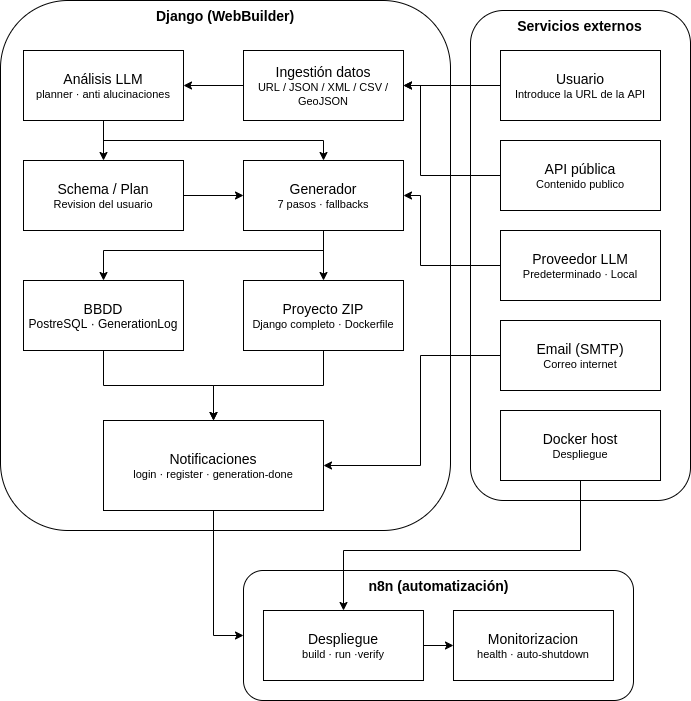
\includegraphics[width=\textwidth]{img/disenoimplementacion/arquitecturageneral}
    \caption{Arquitectura general del sistema WebBuilder}
    \label{fig:arquitectura-general}
\end{figure}

\section{Sprint 1: Definición del proyecto}
\label{sec:definicion-proyecto}

El punto de partida del proyecto fue una reunión con el tutor en abril de 2025, en la que se presentaron posibles ideas.
En esa primera toma de contacto surgieron un par de ideas más, las cuales finalmente se acabaron descartando en nuestra segunda reunión,
ya que decidimos adaptarnos un poco más a la situación actual de las páginas webs y automatizaciones.

\begin{table}[H]
    \centering
    \begin{tabular}{|l|l|p{8cm}|}
        \hline
        \textbf{Reunión} & \textbf{Fecha} & \textbf{Resultado} \\
        \hline
        1ª & Abril 2025 & Presentación de ideas iniciales y definición del enfoque \\
        \hline
        2ª & Julio 2025 & Selección del proyecto final: WebBuilder \\
        \hline
    \end{tabular}
    \caption{Reuniones de definición del proyecto}
    \label{tab:reuniones-definicion}
\end{table}

La primera idea consistía en una aplicación web que, a partir de datos de APIs hospitalarias, ayudara a los pacientes a encontrar el centro 
médico más adaptado a sus necesidades según una serie de parámetros. 
La segunda idea ampliaba esa primera hacia un asistente de mudanza. Esta segunda idea planteaba un escenario sobre un usuario que deseaba instalarse en una ciudad, la aplicación
recogería todos los datos de las APIs públicas y un parseo de los datos proporcionados por agencias y otras empresas, de tal forma que 
introduciendo el usuario sus requisitos, se le organizaría un posible plan de vida en la zona.
Ambas ideas tenían en común la lectura y procesamiento de APIs públicas, pero el alcance era demasiado limitado, haciendo escaso el valor del 
proyecto. 

En la segunda reunión, realizada en Julio de 2025, llegamos a una idea más acotada, una aplicación web Django encargada de procesar los datos
de cualquier API pública y generar automáticamente un sitio web personalizado.

Durante este período fui recogiendo información y creando las posibles fases del sistema:
validación de la URL, procesamiento de los datos recogidos, preferencias sobre el diseño, etc. El tutor valoró positivamente estos pasos, lo que me impulsó para seguir adelante con el proyecto.

Durante los meses de verano el proyecto fue avanzando poco a poco, creando las partes más sencillas para ir dándole forma: la página de inicio, el sistema de login y registro de usuarios. Aunque en el futuro la parte estética cambiaría, la base más o menos se mantendría.

Al principio no hubo un gran desarrollo de código, sino que se dedicó este período a definir con más detalle el flujo de la aplicación, se investigaron tecnologías y se diseñaron procesos que debería seguir el sistema. Este trabajo previo fue muy importante para el correcto desarrollo guiado de la aplicación. Estas tecnologías se explican más en detalle en la siguiente subsección.


\subsection{Tecnologías evaluadas}
\label{subsec:tecnologias-evaluadas}

En este momento se eligió \textbf{Django} como framework backend por su ORM integrado y su compatibilidad con las bibliotecas de procesamiento de datos necesarias, así como la fácil adaptación y escalabilidad de Python.

Para la automatización de flujos asíncronos se consideró la implementación \textbf{n8n} por su capacidad de autoalojamiento y su interfaz visual, aunque su incorporación al proyecto se realizaría más tarde. 

Sobre la integración de LLMs, no se planteó desde el inicio como una posibilidad, aunque más adelante como se describe en la sección~\ref{sec:integracion-llm-n8n} se realizaría su implementación.

\section{Sprint 2: Comienzo del desarrollo}
\label{sec:comienzo-desarrollo}

Con la propuesta del proyecto ya definida, el desarrollo comenzó con fuerza en febrero de 2026. Poco a poco se fue creando la estructura base de 
la aplicación: modelos, sistema de ingestión de datos, lógica de análisis, y una interfaz mínima para poder hacer
pruebas del flujo completo. La arquitectura hasta este punto era bastante sencilla: una aplicación Django que recibía una URL, descargaba los 
datos de la API, los analizaba y devolvía una propuesta de estructura para el futuro sitio web.

\begin{figure}[H]
    \centering
    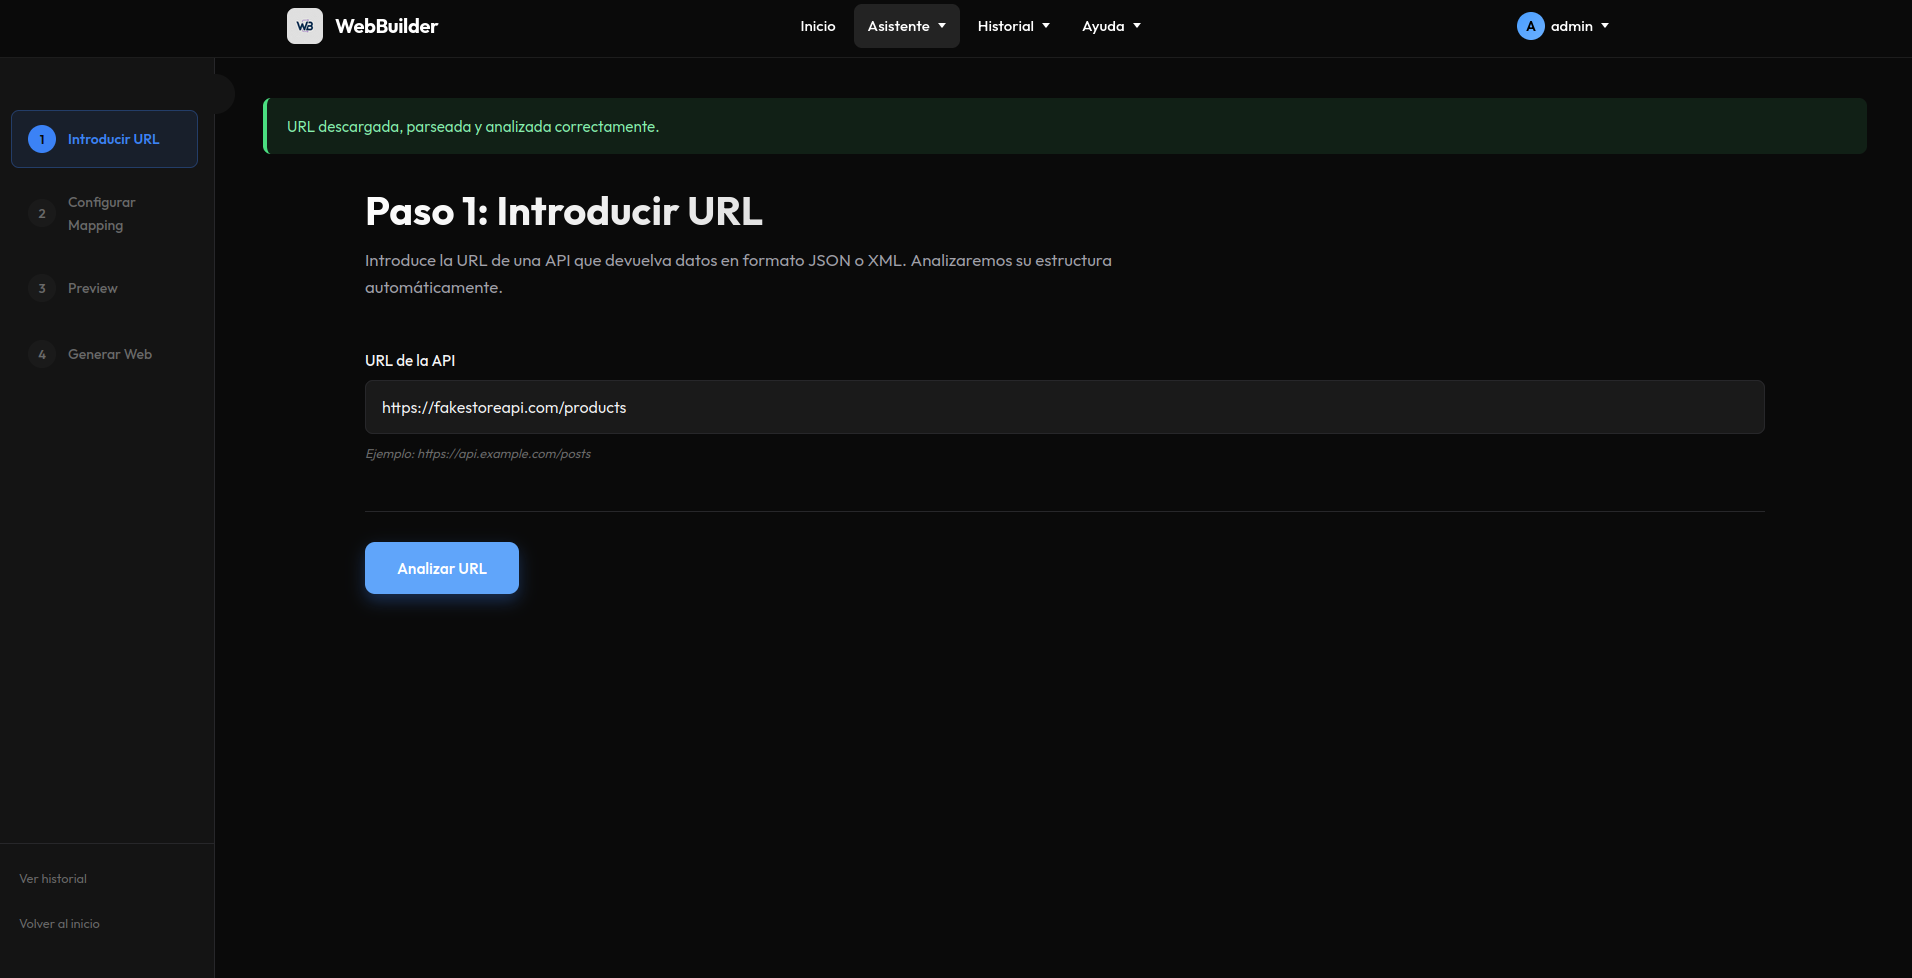
\includegraphics[width=\textwidth]{img/oldversions/urlantigua}
    \caption{Paso 1 del asistente: introducción de la URL de la API}
    \label{fig:urlantigua}
\end{figure}

\begin{figure}[H]
    \centering
    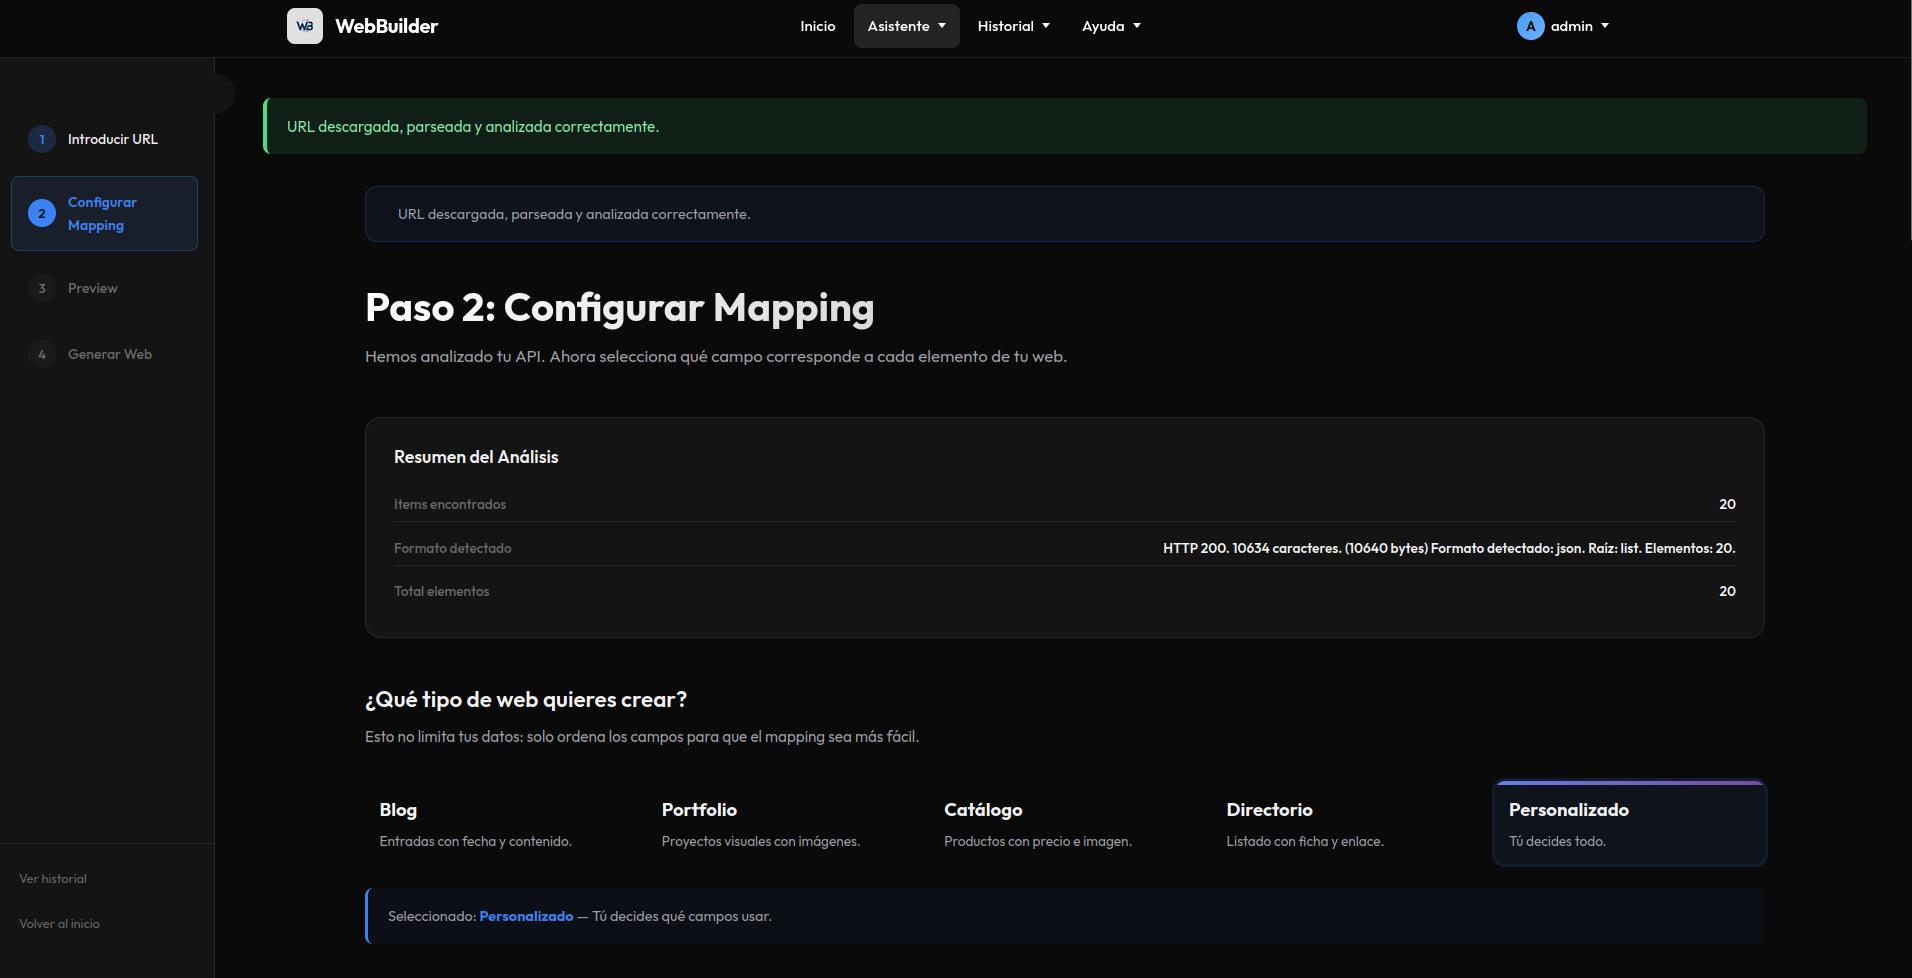
\includegraphics[width=\textwidth]{img/oldversions/heuristicas1}
    \caption{Paso 2 del asistente: configuración del mapping mediante heurísticas}
    \label{fig:heuristicas1}
\end{figure}

\begin{figure}[H]
    \centering
    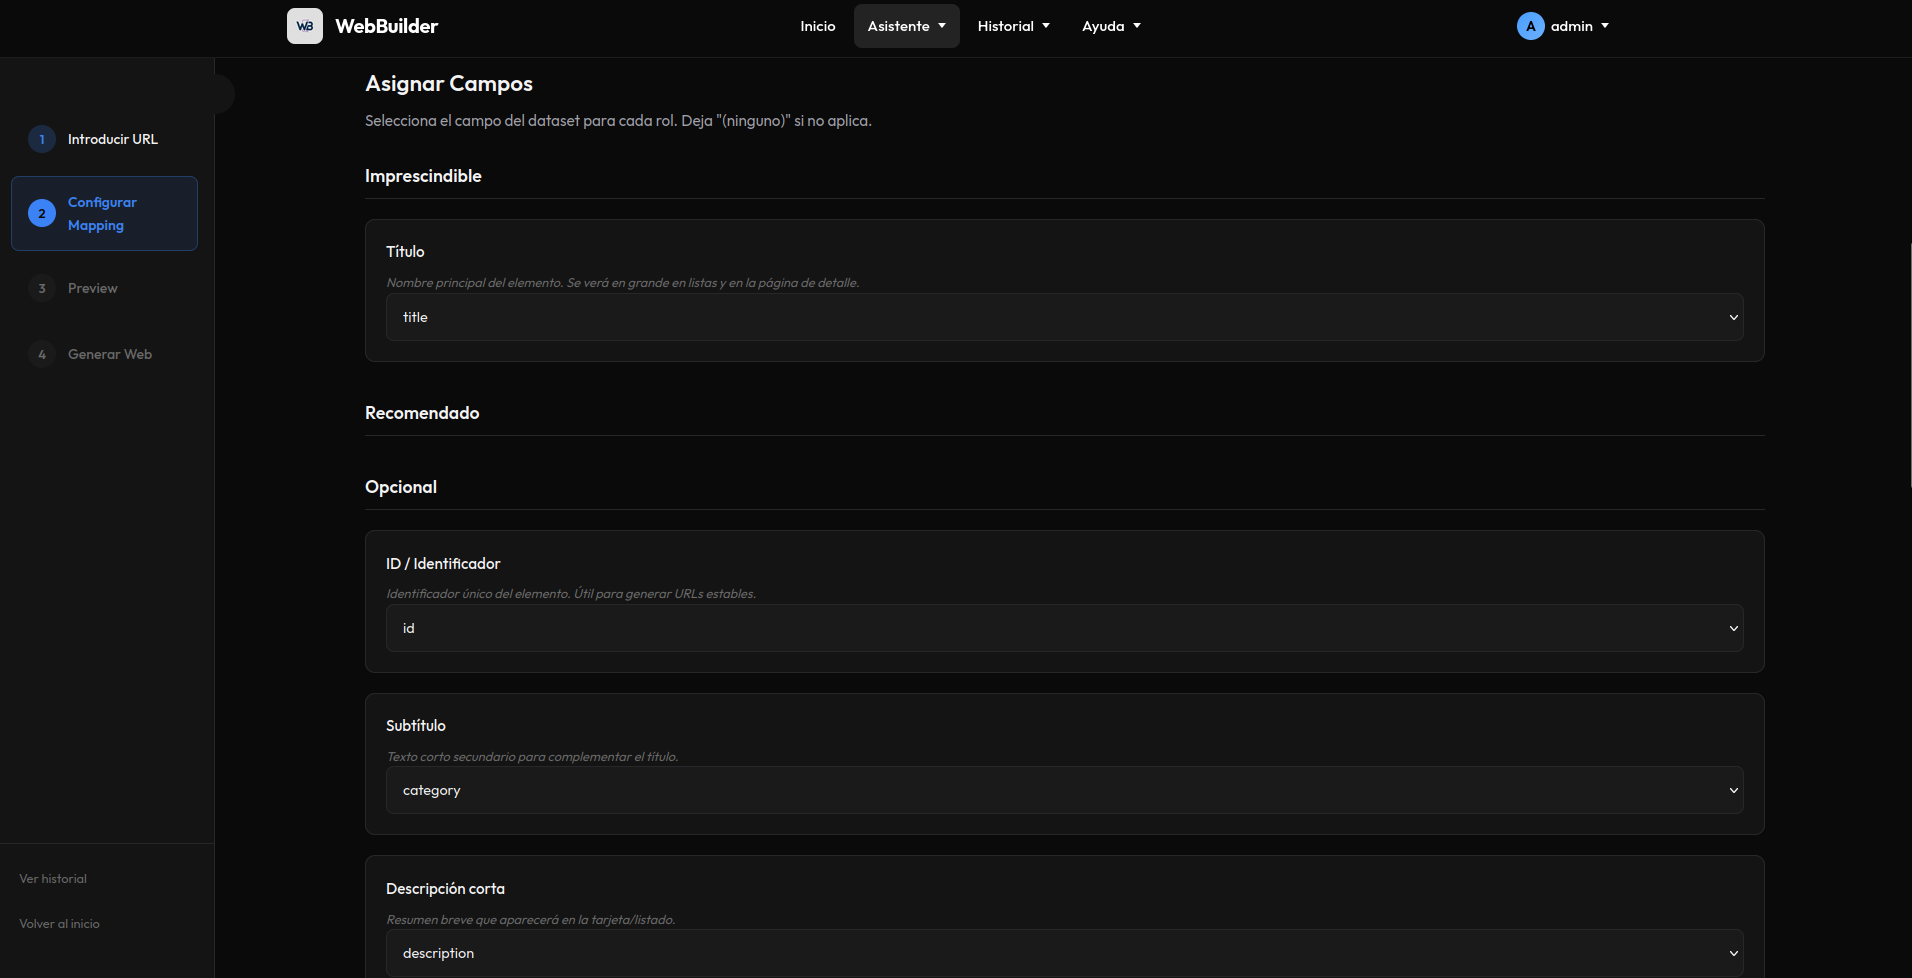
\includegraphics[width=\textwidth]{img/oldversions/heuristicas2}
    \caption{Paso 2 del asistente: asignación manual de campos por roles}
    \label{fig:heuristicas2}
\end{figure}

\subsection{Modelo de datos}
\label{subsec:modelo-datos}

El único modelo de la base de datos en este sprint era \texttt{APIRequest}, que recogía 
los datos de cada petición URL realizada. Sus campos principales se muestran en la 
Tabla~\ref{tab:modelo-apirequest}. Este modelo fue el eje central durante este sprint 
y será la base del análisis durante todo el proyecto.

\begin{table}[H]
    \centering
    \begin{tabular}{|l|l|p{8cm}|}
        \hline
        \textbf{Campo} & \textbf{Tipo} & \textbf{Descripción} \\
        \hline
        url & CharField & URL de la API introducida por el usuario \\
        \hline
        raw\_data & TextField & Datos en crudo descargados de la API \\
        \hline
        parsed\_data & JSONField & Estructura de datos ya parseada \\
        \hline
        status & CharField & Estado del análisis: pending, processed o error \\
        \hline
        field\_mapping & JSONField & Mapping resultante mostrado al usuario \\
        \hline
        created\_at & DateTimeField & Fecha y hora de creación de la petición \\
        \hline
        user & ForeignKey & Usuario propietario del análisis \\
        \hline
    \end{tabular}
    \caption{Campos del modelo APIRequest en la Sprint 2}
    \label{tab:modelo-apirequest}
\end{table}


\subsection{Ingestión de datos}
\label{subsec:ingestion-datos}

El modulo de ingestión de datos, ubicado en \texttt{utils/ingest/} era y será el encargado de validar la URL introducida por el usuario, realizar la descarga del contenido
de forma segura y detectar automáticamente el formato de los datos. La validación comprobaba que la URL procedería de \texttt{http} o \texttt{https}, que fuese
procedente de un dominio válido y que su longitud no superase los 2048 caracteres, límite establecido para evitar ataques mediante URLs maliciosas por su longitud. La descarga se realizaba en modo streaming, es decir, en vez de esperar que
el contenido del archivo se descargue entero, se va leyendo el contenido en fragmentos, cada un con un límite de 1MB, y un timeout de 8 segundos. Conseguimos de 
esta forma evitar que una API con respuestas excesivamente grande nos tumbe o bloquee el sistema.

La detección de formato se realiza inspeccionando los primeros caracteres del contenido de la API, de esta forma se conseguía distinguir entre JSON y XML, que son 
los contenidos manejados hasta este momento, mas adelante en el capítulo~\ref{subsec:nuevos-formatos-entrada} se aumenta el tipo de datos a procesar. En cualquier caso 
siempre se devuelve una estructura Python homogénea, que se utiliza en adelante para el sistema, de forma que no es necesario seguir trabajando con el formato 
original.

\subsection{Detección de la colección principal}
\label{subsection:deteccion-coleccion-principal}

La parte mas compleja de este sprint fue entender la estructura interna de los campos de las distintas APIs. Los campos de las APIs no suelen ser una lista plana de items
en la raíz, es decir, la colección principal no esta expuesta, sino que esta envuelta bajo claves de metadatos como \texttt{results}, \texttt{data} o \texttt{items},
o incluso con varios niveles de profundidad. 

Para resolver esto se implementó un nuevo modulo: \texttt{utils/analysis}, donde se crearon ficheros con funciones importantes como \texttt{find\_main\_items}, la cual recorría recursivamente la estructura de la API, y se evaluaba con un sistema de puntuación propio para sacar la estructura principal.

Cada lista candidata se puntuaba según cinco factores:

\begin{itemize}
    \item \textbf{Densidad de diccionarios}: porcentaje de elementos de la lista que son diccionarios. Las listas con menos de un 55\% de dicts recibían una penalización proporcional, ya que era poco probable que representaran una colección de entidades reales.
    \item \textbf{Tamaño}: listas con más items recibían mayor puntuación, aunque con un límite para evitar que una lista enorme pero trivial se impusiera sobre una colección más pequeña pero más relevante.
    \item \textbf{Consistencia de claves}: si todos los diccionarios de la lista compartían aproximadamente las mismas claves, era muy probable que representaran entidades del mismo tipo. Se calculaba como el promedio de claves propias de cada item sobre la unión de todas las claves observadas.
    \item \textbf{Bonus por claves semánticas}: si los campos de la colección incluían nombres típicos de contenido como \texttt{title}, \texttt{name}, \texttt{id},    \texttt{description} o \texttt{image}, se añadía una bonificación proporcional al número de coincidencias.
    \item \textbf{Penalización por profundidad}: los paths muy anidados o que pasaban por índices numéricos se penalizaban para favorecer colecciones cercanas a la raíz, que solían ser las más relevantes.
\end{itemize}

Al finalizar este scoring, se seleccionaba la lista con mayor puntuación como 
colección principal, junto con la ruta dentro de la estructura original. En la 
Figura~\ref{fig:sistema-scoring} se muestra cómo los cinco factores se combinan 
en la función de scoring para obtener la colección principal.

\begin{figure}[H]
    \centering
    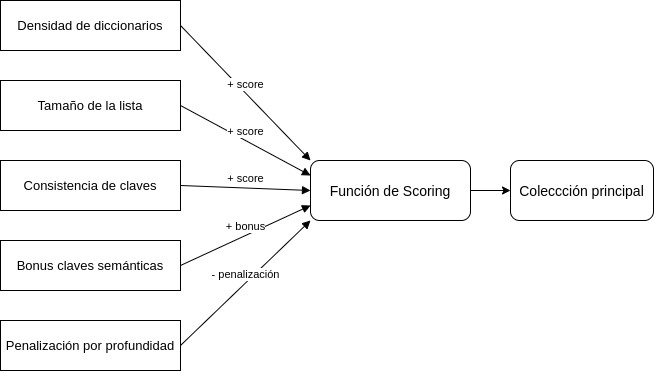
\includegraphics[width=0.7\textwidth]{img/disenoimplementacion/sistemascoring}
    \caption{Sistema de scoring para la detección de la colección principal}
    \label{fig:sistema-scoring}
\end{figure}


\subsection{Sugerencia automática}
\label{subsec:sugerencia-automatica}

Una vez localizada la colección principal, se realizo la implementación del nuevo fichero \textbf{utils/mapping.py}, encargado de sugerir automáticamente que campos
del dataset debían ocupar cada rol: fecha, id, descripción, etc. Para ello se utilizaba un catalogo predefinido que asociaba cada rol con sus nombres más habituales.
Por ejemplo un campo llamado \texttt{published\_at}, obtenía un alto score para el rol fecha ya que contenía la subcadena \texttt{published}.
Además de la comparación por nombre, el sistema añadía score extra si el tipo del campo observado coincidía con el tipo esperado en el rol.

Para evitar que la misma clave del dataset se asignara como primera sugerencia de varios roles a la vez, se implementó una función llamada \texttt{suggest\_mapping}, que aplicaba una asignación por orden de prioridad: primero se reservaba la mejor clave para el rol \texttt{id}, luego para \texttt{title}, luego para \texttt{description}, y así sucesivamente. Esto reducía la repetición de sugerencias y hacía el mapping resultante más útil para el usuario, sin embargo, ocurrían errores como que algunos campos se quedasen vacíos o que al asignarse por orden de prioridad, algunos campos sueltos se asignasen a roles
que no tenían relación.



\subsection{Elección pagina}
\label{subsec:eleccion-pagina}

Para guiar mejor al usuario durante el proceso de mapping, se añadió un sistema de perfiles de intención en \texttt{intents.py}. El usuario podía indicar si quería construir un blog, un portfolio, un catálogo o un directorio, y el sistema reordenaba los roles y ajustaba cuáles eran obligatorios, recomendados u opcionales según ese tipo de sitio.
Se puede observar en las Figuras~\ref{fig:heuristicas1} y~\ref{fig:heuristicas2} 
cómo el sistema solicitaba al usuario configurar el tipo de pagina y los campos.

\subsection{Calidad del mapping}
\label{subsec:calidad-mapping}
Además, se implementó un sistema de puntuación de calidad del mapping en \texttt{mapping.py}, que evaluaba de 0 a 100 el mapping introducido por el usuario teniendo en cuenta si había asignado los roles más importantes, si existían duplicados entre roles críticos y qué campos quedaban vacíos. El resultado se mostraba al usuario con una etiqueta cualitativa: \emph{Excelente}, \emph{Bueno}, \emph{Aceptable} o \emph{Mejorable}.


\subsection{Tests}
\label{subsec:test1}

Desde el primer sprint se escribieron tests para los cuatro módulos principales 
del sistema heurístico, organizados en ficheros independientes: 
\texttt{test\_analysis}, \texttt{test\_mapping}, \texttt{test\_normalizer} 
y \texttt{test\_parsers}. Estos test cubrían casos como la detección de colecciones anidadas, la asignación de roles por prioridad, la normalización de valores y el parseo seguro de XML. Esto permitió verificar el comportamiento del sistema de scoring con datasets variados, detectando casos en los que las heurísticas fallaban antes de que llegaran al usuario.

\subsection*{Limitaciones del enfoque heurístico} 
\label{subsec:limitaciones1}

Conforme se probaba el sistema con datasets reales muy distintos entre sí, los límites del enfoque heurístico se fueron haciendo evidentes. Una API de plantas medicinales, una de personajes de ficción y una de productos de e-commerce tienen nomenclaturas de campos completamente diferentes, y un sistema de reglas fijas no podía cubrir todos los casos con la misma fiabilidad. Cuando los nombres de los campos no coincidían con los campos de la API, el mapping era genérico y malo para el usuario. El sistema funcionaba razonablemente bien con APIs convencionales y con campos estándar, pero fallaba ante cualquier dataset con nombres o estructura poco habituales. Esta limitación fue la que motivó el cambio de enfoque descrito en el siguiente sprint.



\section{Sprint 3: Integracion LLM y n8n}
\label{sec:integracion-llm-n8n}

Con el sprint 2 terminada y viendo que las limitaciones eran evidentes, se tomó la decisión de realizar un cambio fundamental para el futuro del proyecto. Se abandonó 
la idea del sistema de reglas, aunque no en la totalidad, ya que algunas partes nos seguirían siendo útiles. Se decidió integrar un
modelo de lenguaje (LLM) como núcleo o motor del análisis y generación de las páginas. Hasta este momento el sistema intentaba entender los datos mediante
puntuaciones y comparaciones. A partir de este punto, se decidió que fuese la Inteligencia Artificial la encargada de escoger y proponer la estructura del sitio y decidiera que 
campos mostrar. Como se comentó anteriormente, no todo el flujo de análisis e ingesta se cambió, se eliminaron las partes de score y propuesta de dataset, pero el parseo 
y análisis de los campos se mantuvo y modificó levemente, se introdujo todo el dataset en una estructura, que sería la que se pasaría al LLM, de forma que evitaríamos
alucinaciones o errores del LLM en la lectura de la API, obteniendo de esta forma un schema más consistente. Este proceso se describe con más detalle en la subsección~\ref{subsec:proteccion-anti-alucionaciones}


\subsection{Conexión con LLM}
\label{subsec:conexion-llm}

Para poder realizar la conexión con el LLM, el primer paso fue crear el módulo \textbf{utils/llm}, y dentro se creó el archivo \texttt{client.py}, el cual
implementa la función \texttt{chat\_completions}. Esta función se encarga de hacer una única cosa: enviar un mensaje al LLM y devolver la respuesta en texto
plano.

Una decisión importante fue utilizar el estándar de la mayoría de proveedores para realizar la conexión, utilizando de esta forma el endpoint \textbf{/chat/completions}. En este caso creado para poder realizar pruebas con varios LLM de diferentes proveedores (OpenRouter, Groq, NVIDIA) y cualquier agente local.
Otra decisión fue crear \texttt{.env}, de forma que la URL base, la API key y el modelo se leen de variables de entorno definidas en dicho fichero, lo que permite cambiar de proveedor sin tocar una sola línea de código.

La función mencionada anteriormente acepta tres parámetros principales:

\begin{itemize}
    \item \textbf{Mensaje de usuario}: la tarea concreta que se le envía al modelo 
    en cada llamada, en este caso el prompt con los datos del dataset, las claves 
    disponibles y los ejemplos de items reales.
    
    \item \textbf{Mensaje de sistema}: instrucciones previas que definen cómo debe 
    comportarse el modelo antes de procesar el mensaje del usuario. Se utiliza para 
    indicarle el rol que debe adoptar, el formato de respuesta esperado y lo que 
    está prohibido hacer. Es opcional, ya que técnicamente todo puede ir en el 
    mensaje de usuario, pero separarlo es una buena práctica que facilita reutilizar 
    el mismo comportamiento base en distintas llamadas. Por ejemplo, el mensaje de sistema del planner indica al modelo que es un experto en diseño 
    de sitios web, que debe devolver únicamente un objeto JSON válido y que está 
    prohibido inventar campos que no existan en el dataset proporcionado.
    
    \item \textbf{Temperatura}: parámetro que controla el grado de aleatoriedad 
    en las respuestas del modelo. Un valor cercano a 0 produce respuestas más 
    deterministas y predecibles, mientras que valores más altos generan respuestas 
    más creativas pero menos consistentes. En este caso se fija por defecto en 
    \texttt{0.2}, favoreciendo la estabilidad especialmente cuando se espera JSON 
    estructurado como salida.
\end{itemize}

El primer proveedor utilizado fue OpenRouter, con el modelo de meta-llama: \\
\texttt{llama-3.3-70b-instruct:free}, de acceso gratuito y potencia más que suficiente para las primeras pruebas.

% Meter captura de ejemplo de prompt

\begin{figure}[H]
    \centering
    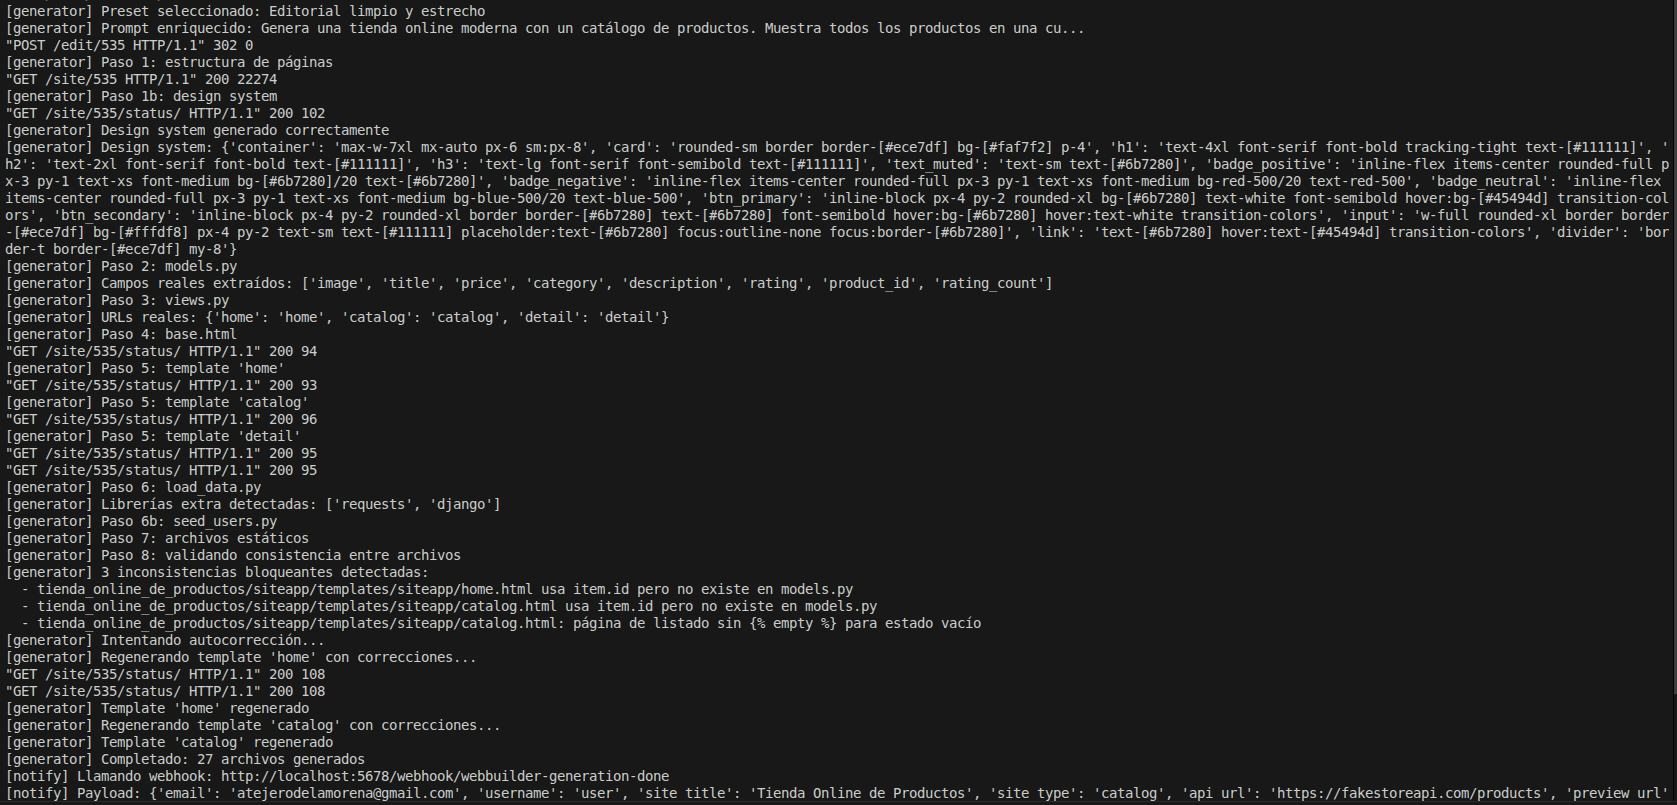
\includegraphics[width=1\textwidth]{img/webbuilder/disenoimplementacion/logs-generacion.png}
    \caption{Ejemplo logs de generación de proyecto}
    \label{fig:Ejemplo logs de generacion}
\end{figure}

\subsection{Planner schema}
\label{subsec:planner-schema}

Otro fichero clave fue \texttt{utils/llm/planner.py} y su función \texttt{generate\_site\_plan}. La misión era transformar el resultado del análisis en un propuesta con campos
concretos de schema que el usuario pudiese aceptar y modificar a su gusto antes de continuar.

El schema tiene una forma fija que el resto del sistema espera:
\begin{itemize}
    \item \textbf{site\_type}: tipo de sitio recomendado, entre \texttt{blog}, \texttt{portfolio}, \texttt{catalog}, \texttt{dashboard} u \texttt{other}.
    \item \textbf{site\_title}: nombre descriptivo del sitio propuesto por el modelo.
    \item \textbf{fields}: lista ordenada de campos del dataset que el sitio debe mostrar, cada uno con su clave original y una etiqueta legible para el usuario.
\end{itemize}

Para obtener este esquema, se construye un prompt estructurado que se envía al LLM. Este prompt es el resultado de una serie de pruebas con distintas formulaciones,  
siguiendo técnicas de \emph{prompt engineering}~\cite{openai_prompt_engineering} para conseguir respuestas consistentes y parseables. La información contenida en este 
prompt es la siguiente:

\begin{itemize}
    \item \textbf{Objetivo del usuario}: texto en lenguaje natural introducido por 
    el usuario describiendo qué tipo de sitio quiere construir.
    
    \item \textbf{Claves disponibles}: lista de campos reales extraídos del dataset 
    durante la fase de análisis. El modelo solo puede proponer campos que estén 
    en esta lista.
    
    \item \textbf{Ejemplos del dataset}: hasta tres items reales del dataset, para 
    que el modelo pueda entender qué tipo de valores contiene cada campo y proponer 
    etiquetas adecuadas.
    
    \item \textbf{Contrato JSON}: estructura exacta que debe devolver el modelo, 
    con los campos obligatorios y su formato esperado.
    
    \item \textbf{Reglas de formato}: conjunto de instrucciones explícitas que 
    indican al modelo que debe devolver únicamente un objeto JSON válido, sin 
    bloques de código Markdown, sin texto introductorio y sin ningún contenido 
    fuera del JSON.
\end{itemize}

Esta rigidez sobre el formato de salida es intencionada, ya que tras la 
realización de varias pruebas, los fallos generados por los diferentes LLM 
siempre eran parecidos. Como esa respuesta se usa directamente en el sistema, 
cualquier texto adicional rompe el proceso de parseo.

De todas formas, debido a las alucinaciones de algunos modelos y a que en 
ocasiones ignoraban las restricciones de formato, se aplicaba una limpieza 
previa sobre la respuesta antes de parsearla. Esta limpieza eliminaba bloques 
de código Markdown como \texttt{```json} o \texttt{```}, que algunos modelos 
añaden automáticamente alrededor del JSON aunque se les indique explícitamente 
que no lo hagan, así como espacios y caracteres sobrantes al inicio y al final 
de la respuesta, los cuales rompían el flujo de ejecución del proyecto.


\begin{figure}[H]
    \centering
    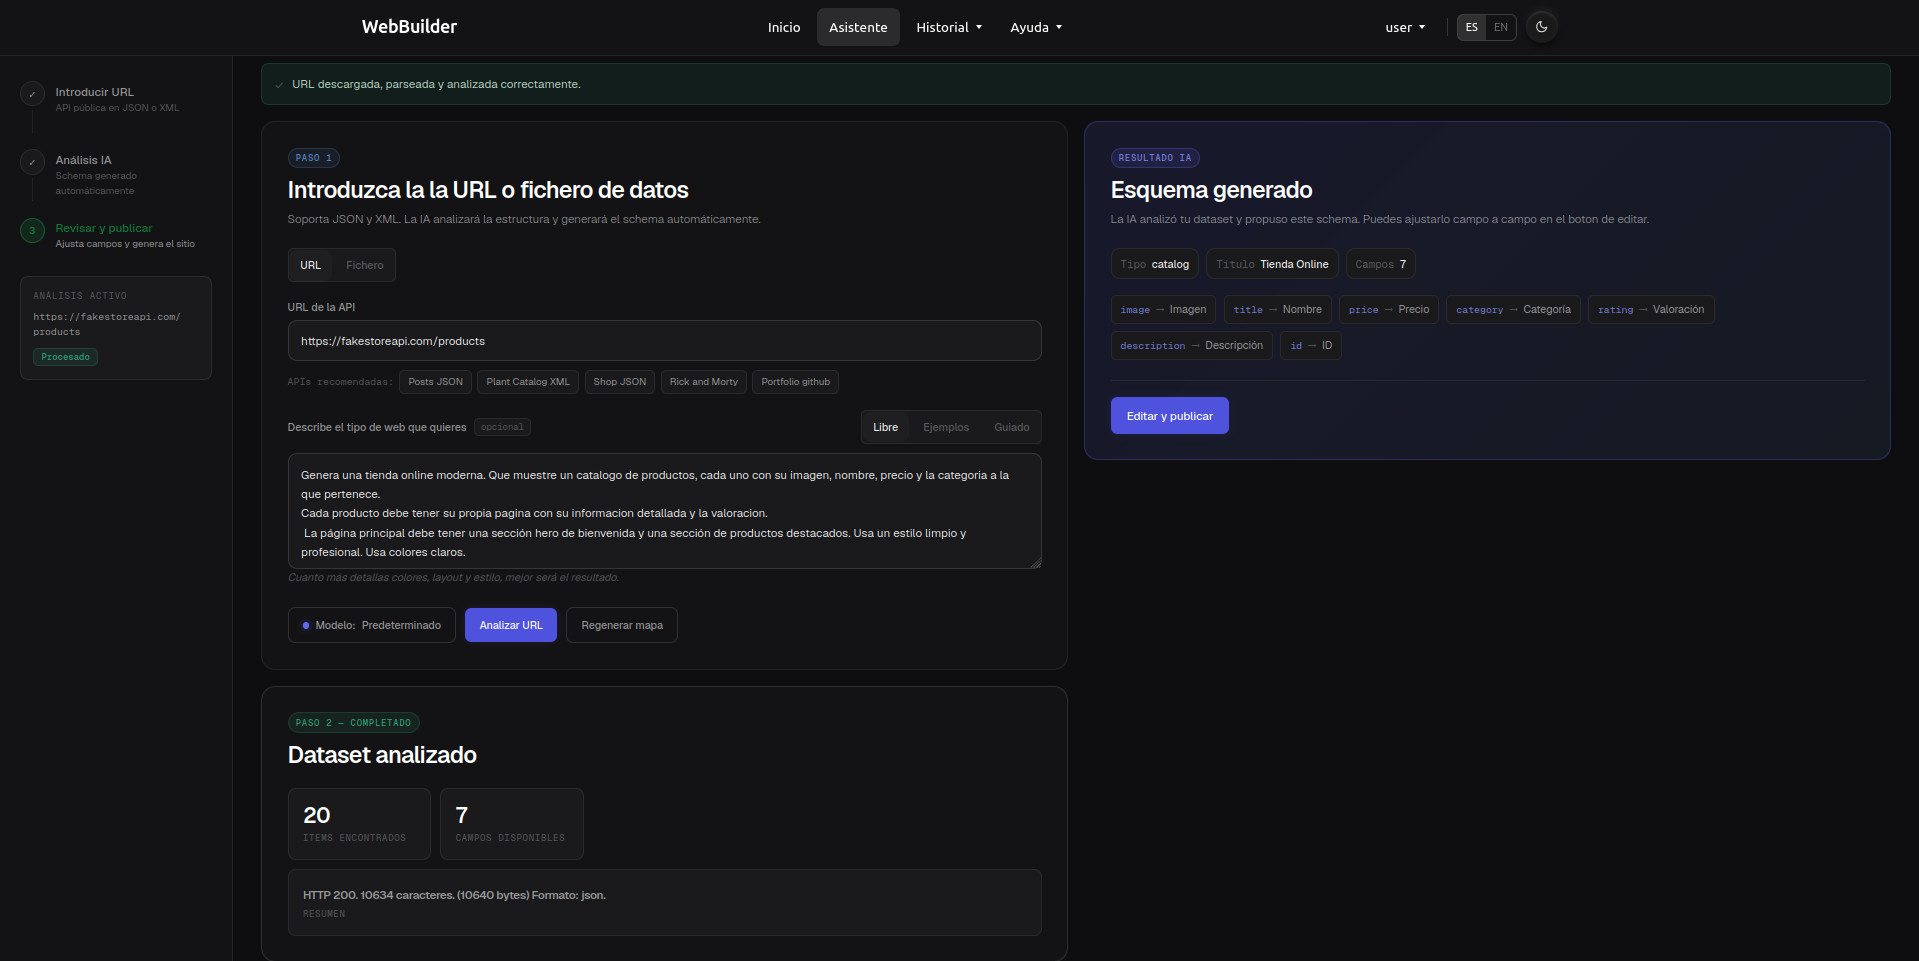
\includegraphics[width=\textwidth]{img/webbuilder/disenoimplementacion/asistente-schema.png}
    \caption{Schema generado automáticamente por el LLM a partir de la API analizada}
    \label{fig:asistente-schema}
\end{figure}

\subsection{Protección anti-alucinaciones}
\label{subsec:proteccion-anti-alucionaciones}

Los errores más comunes siempre sucedían por la misma causa, las alucinaciones del LLM. El error más común era inventar información que no existía en la API, y que nunca se parseo, por lo que no existe en el dataset construido. Para ello hubo que aplicar varias capas de defensa contra alucinaciones para proteger los schemas.

\begin{itemize}
    \item \textbf{Validación contra claves reales}: cada clave propuesta por el LLM se comprueba contra la lista de claves reales extraída del dataset. Si la clave no existe, se intenta un match sin distinguir mayúsculas y minúsculas. Si tampoco hay coincidencia, la clave se descarta silenciosamente.

    \item \textbf{Filtro de tokens prohibidos}: existe una lista de palabras que 
    el modelo confunde con claves del dataset porque forman parte del propio prompt del usuario. 
    Al estar palabras como \texttt{available\_keys}, \texttt{fields} o 
    \texttt{examples} presentes en el texto del prompt, algunos modelos las 
    interpretan erróneamente como campos reales del dataset y las incluyen en su 
    respuesta. Por ejemplo, si el prompt contiene la línea 
    \texttt{"available\_keys": ["name", "date", "url"]}, el modelo puede devolver 
    \texttt{available\_keys} como uno de los campos seleccionados, cuando en 
    realidad es una etiqueta del propio prompt. Cualquier clave que coincida con 
    esta lista se descarta automáticamente.
    
    \item \textbf{Detección de valores disfrazados de claves}: se detectan los 
    casos en los que el modelo introduce un valor concreto del dataset donde 
    debería haber puesto el nombre de un campo. Por ejemplo, si el dataset tiene 
    un campo de fecha, el modelo puede devolver \texttt{2024-01-15} como clave 
    en lugar de \texttt{published\_at}. Para evitarlo, se descartan 
    automáticamente cadenas que sean fechas en formato ISO, URLs completas, 
    extensiones de imagen, valores nulos o texto excesivamente largo.
    
    \item \textbf{Fallback}: si tras aplicar todas las validaciones no queda ninguna clave válida, el sistema construye automáticamente un schema de emergencia con las primeras claves del dataset, garantizando que el flujo nunca se bloquea por un fallo del modelo.
\end{itemize}

Si el parseo falla, el sistema reintenta automáticamente una vez con una pista sobre el error cometido. Si el segundo intento también falla, se activa el fallback. En la Figura~\ref{fig:flujo-url-schema} se muestra el flujo completo desde que el usuario introduce la URL hasta obtener el schema validado.

\begin{figure}[H]
    \centering
    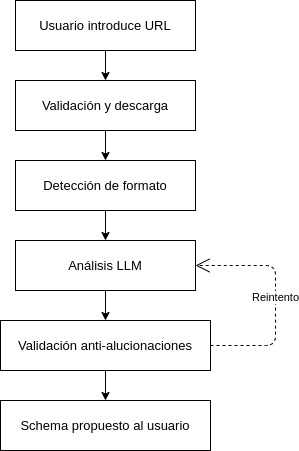
\includegraphics[width=0.4\textwidth]{img/disenoimplementacion/flujourlfase3}
    \caption{Flujo de ingestión y análisis}
    \label{fig:flujo-url-schema}
\end{figure}

\subsection{Actualización de modelos}
\label{subsec:actualizacion-modelos}

La integración del LLM trajo consigo dos cambios importantes.

El primero de ellos fue una modificación en el modelo existente \textbf{APIRequest}, añadiéndole el campo \texttt{plan\_accepted}. Siendo este un booleano encargado de guardar
si el usuario ha aceptado el schema propuesto antes de continuar.

El segundo fue la creación de un nuevo modelo \textbf{GeneratedSite}, 
vinculado con el modelo \texttt{APIRequest} mediante una relación 
\texttt{OneToOne}. Sus campos principales se muestran en la 
Tabla~\ref{tab:modelo-generatedsite}.

\begin{table}[H]
    \centering
    \begin{tabular}{|l|l|p{8cm}|}
        \hline
        \textbf{Campo} & \textbf{Tipo} & \textbf{Descripción} \\
        \hline
        api\_request & OneToOneField & Referencia al análisis que originó el sitio \\
        \hline
        public\_id & UUIDField & Identificador único público del sitio generado \\
        \hline
        plan & JSONField & Schema aceptado por el usuario con los campos seleccionados \\
        \hline
        project\_files & JSONField & Ficheros del proyecto generado indexados por ruta \\
        \hline
    \end{tabular}
    \caption{Campos principales del modelo GeneratedSite en el sprint 3}
    \label{tab:modelo-generatedsite}
\end{table}

\subsection{Integración de n8n}
\label{subsec:integracion-n8n}

En paralelo a la integración del LLM, durante este sprint se incorporó n8n al sistema por primera vez. Es una herramienta de automatización de flujos que permite conectar servicios mediante webhooks y nodos, y que más adelante sería una pieza fundamental de la arquitectura del proyecto. En este momento su uso fue todavía inicial: instalar el entorno y crear el primer flujo de pruebas.

n8n se instaló en un contenedor Docker siguiendo la imagen oficial, quedando disponible en \texttt{localhost:5678}. Una vez levantado el entorno, se creó el primer flujo en n8n y se configuró el primer webhook, apuntando a la ruta \texttt{/webhook-test/WebBuilder-Register}. El prefijo \texttt{webhook-test} indica que el webhook estaba en modo de prueba, el modo que n8n ofrece para verificar que el flujo funciona correctamente antes de activarlo en producción.

La integración en Django se realizó en \texttt{views/auth.py}, donde se añadió la función\texttt{llamar\_webhook}. El nodo se encargaría de notificar a los usuarios recién registrados: Django realizaba una llamada POST a ese webhook con el nombre de usuario y el email del recién registrado, y n8n enviaba automáticamente un correo de bienvenida 
personalizado a esa dirección. Más adelante se completaría el flujo con el webhook de login.

La función estaba diseñada para ser completamente transparente al flujo principal: si n8n no estaba disponible o la llamada fallaba, la excepción se capturaba silenciosamente y el registro continuaba con normalidad. Esto garantizaba que un fallo en el sistema de notificaciones nunca pudiera bloquear el acceso a la aplicación.


\begin{figure}[H]
    \centering
    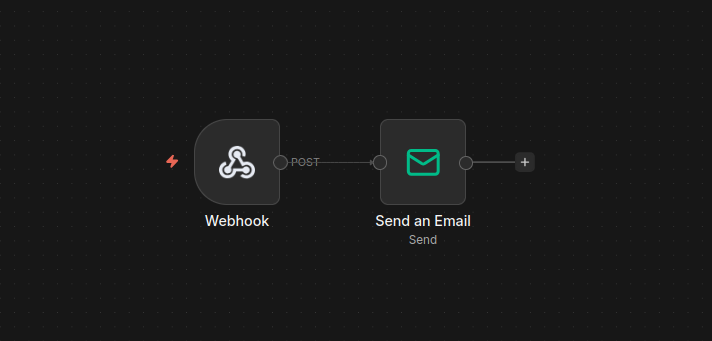
\includegraphics[width=0.7\textwidth]{img/n8n/login-register.png}
    \caption{Flujo n8n login y register}
    \label{fig:Flujo n8n login y register}
\end{figure}
\section{Sprint 4: Generador de proyectos Django}
\label{sec:generador-proytectos}

Tras la implementación del LLM y el sistema de schema funcionando correctamente, el siguiente paso era el más complejo del proyecto, ya que requería 
coordinar múltiples llamadas al LLM de forma secuencial garantizando 
que cada fichero generado fuese compatible con los anteriores. Dicho paso era convertir el schema aprobado por el usuario en un proyecto Django completo, funcional y desplegable. Durante este sprint del proyecto surgió el fichero más importante hasta la fecha: \textbf{utils/generator/project\_generator}, el núcleo de WebBuilder.


\subsection{Arquitectura del generador}
\label{subsec:arquitectura-generador}

El generador se organiza como un orquestador de siete pasos secuenciales, cada uno con su responsabilidad concreta y encargado de producir uno o varios ficheros del proyecto final.
El LLM interviene en los primeros seis pasos, que se encargan de la creación de ficheros, pero en el séptimo paso ya no interviene, y se concluye la ejecución con el ensamblaje de todos los ficheros generados anteriormente.

\begin{itemize}
    \item \textbf{Paso 1 — Estructura de páginas}: decide qué páginas 
    tendrá el sitio, sus URLs, sus nombres de vista y si cada página es 
    un listado, una página de detalle o una portada. El resultado guiará 
    todos los pasos siguientes.
    
    \item \textbf{Paso 2 — models.py}: genera el modelo de datos Django 
    adaptado a los campos del dataset.
    
    \item \textbf{Paso 3 — views.py y urls.py}: genera las vistas para 
    cada página del paso 1. El fichero \texttt{urls.py} se construye en 
    Python directamente a partir de la lista de páginas, sin intervención 
    del modelo.
    
    \item \textbf{Paso 4 — base.html}: genera la plantilla base con la 
    estructura HTML común: cabecera, navegación y bloque de contenido.
    
    \item \textbf{Paso 5 — Templates por página}: genera un template HTML 
    independiente para cada página, adaptado a su tipo y a los campos del 
    dataset.
    
    \item \textbf{Paso 6 — load\_data.py}: genera un comando de gestión 
    Django que descarga los datos de la API original y los inserta en la 
    base de datos del sitio generado, garantizando contenido real desde 
    el primer arranque.
    
    \item \textbf{Paso 7 — Archivos fijos}: se ensamblan los ficheros de 
    infraestructura independientes del dataset: \texttt{settings.py}, 
    \texttt{manage.py}, \texttt{wsgi.py}, \texttt{requirements.txt}, 
    \texttt{Dockerfile} y \texttt{entrypoint.sh}.
\end{itemize}


Como ejemplo representativo, se muestra el prompt que se envía 
al LLM en el Paso 2 para la generación del fichero \texttt{models.py}. 
A diferencia de prompts más abiertos, este es restrictivo, la causa es que el código generado debe ser sintácticamente correcto sin ninguna intervención humana, por lo que cada regla busca eliminar un tipo 
de error concreto observado durante las pruebas.

\begin{lstlisting}[caption={Prompt de sistema para la generación de models.py}, 
label={lst:models-system}]
Eres un desarrollador Django experto en Python y Tailwind CSS.
REGLA ABSOLUTA: devuelves ÚNICAMENTE código puro, sin ningún tipo de 
Markdown. Sin ```, sin ```python, sin explicaciones. Solo el código.
\end{lstlisting}

\begin{lstlisting}[caption={Prompt de usuario para la generación de models.py}, 
label={lst:models-user}]
SITIO: <nombre del sitio>

CAMPOS:
[{"key": "campo1", "label": "Etiqueta 1"}, ...]

ROLES SEMÁNTICOS INFERIDOS (clave: rol):
  - campo1: title
  - campo2: numeric
  - campo3: image

DATOS DE EJEMPLO:
[{"campo1": "valor1", "campo2": 42, ...}, ...]

REGLAS:
- CRÍTICO: tu respuesta debe empezar EXACTAMENTE con
  'from django.db import models'. Sin nada antes.
- Un modelo llamado 'Item' con los campos del schema.
- rol 'numeric'   -> FloatField(null=True, blank=True)
- rol 'image'     -> URLField(max_length=500, blank=True)
- rol 'date'      -> DateField(null=True, blank=True)
- rol 'boolean'   -> BooleanField(null=True, blank=True)
- rol 'long_text' -> TextField(blank=True)
- rol 'title'     -> CharField(max_length=300, blank=True)
- rol 'text'      -> CharField(max_length=500, blank=True)
- Todos los campos opcionales (blank=True / null=True).
- Añade created_at = models.DateTimeField(auto_now_add=True).
- __str__ devuelve el campo más representativo.
- NUNCA uses JSONField ni CharField para listas.

\end{lstlisting}

El resultado final es un diccionario Python donde cada clave es una ruta relativa de fichero y cada valor es su contenido. Este diccionario se guarda en el campo \texttt{project\_files} del modelo \texttt{GeneratedSite}, comentado más adelante en la subsección~\ref{subsec:modelo-generatedsite}

A modo de ejemplo, la Figura~\ref{fig:Primera-generación} muestra el resultado de una 
de las primeras generaciones reales del sistema, utilizando la API pública 
\texttt{fakestoreapi.com/products}, que devuelve un catálogo de productos 
con campos como título, precio, categoría e imagen. El sitio generado, aunque 
funcional, refleja las limitaciones del generador: 
diseño genérico, campos mostrados en crudo, sin estilos visuales y sin las imágenes de la base de datos.

\begin{figure}[H]
    \centering
    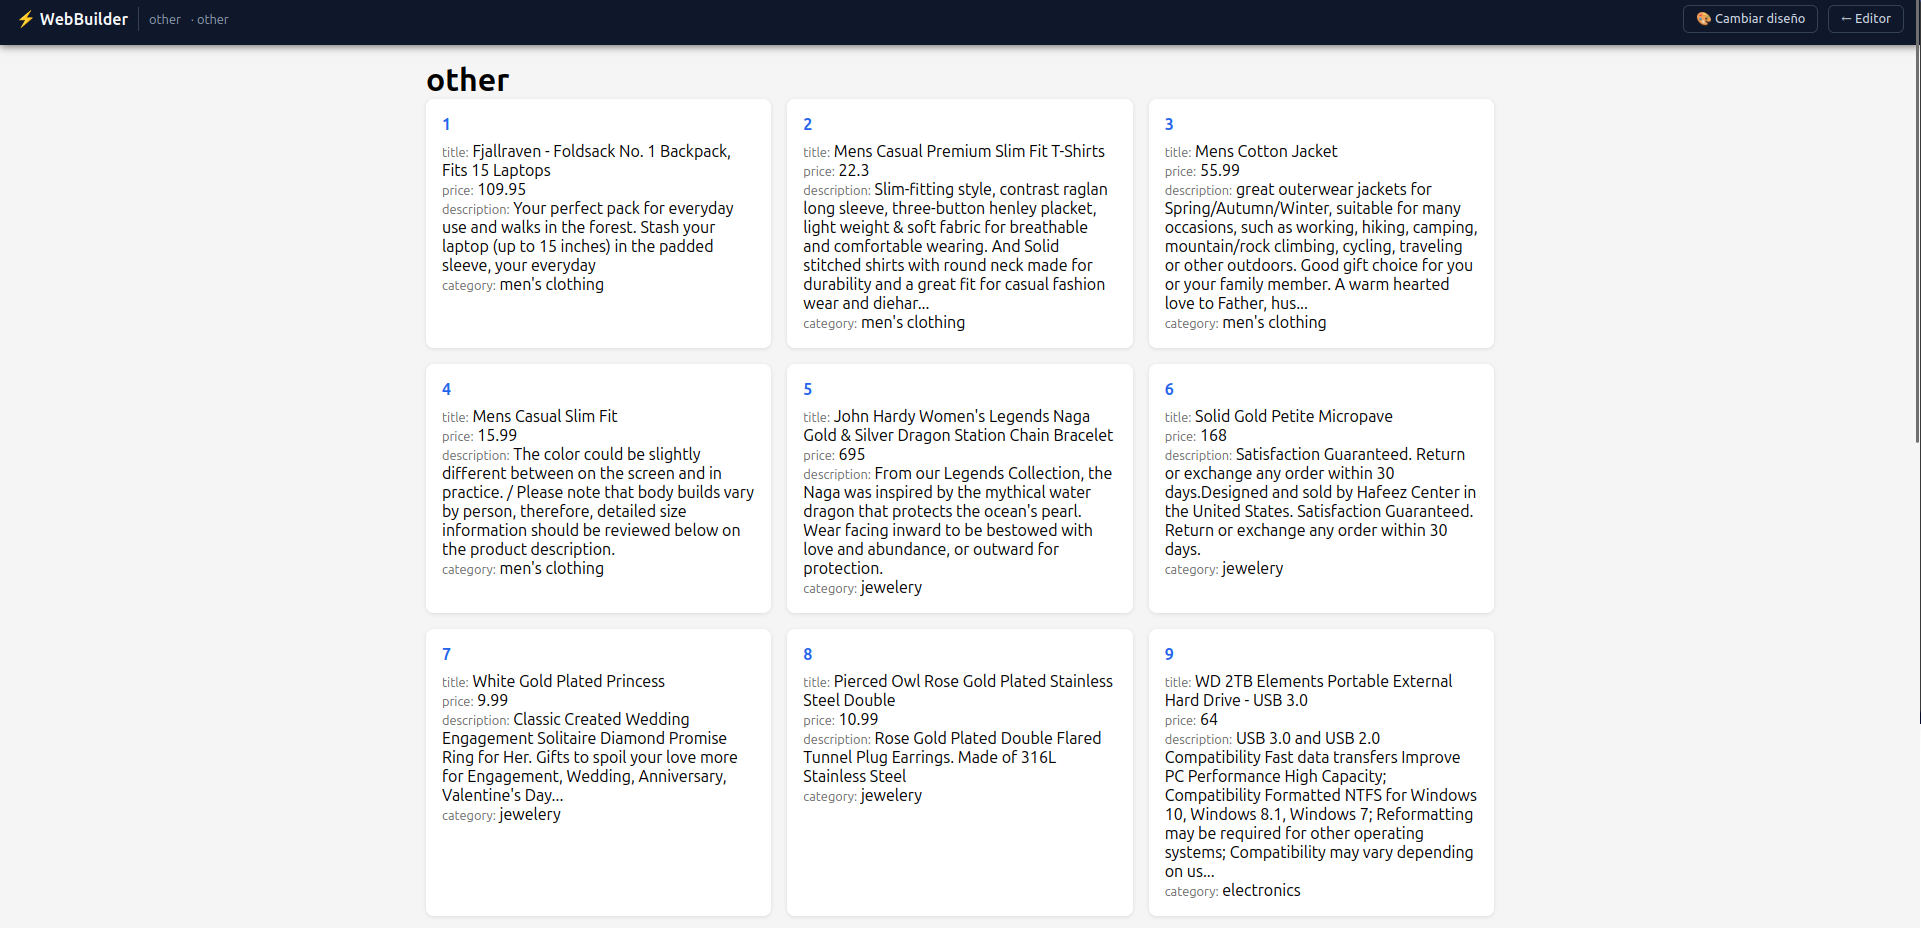
\includegraphics[width=\textwidth]{img/oldversions/firstgenPRODUCTS}
    \caption{Primera web generada por WebBuilder a partir de la API FakeStore}
    \label{fig:Primera-generación}
\end{figure}

En la Figura~\ref{fig:generador-7-pasos} se muestra la secuencia completa de los siete pasos del generador.

\begin{figure}[H]
    \centering
    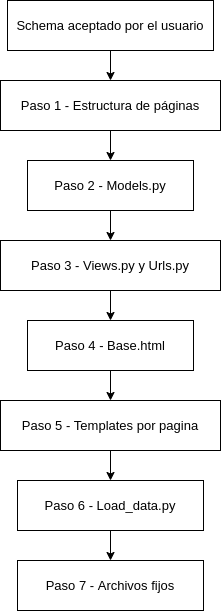
\includegraphics[width=0.3\textwidth]{img/disenoimplementacion/pasosgeneradorfase4.png}
    \caption{Los 7 pasos del generador de proyectos Django}
    \label{fig:generador-7-pasos}
\end{figure}

\subsection{Fallbacks de generación}
\label{subsec:fallbacks-generacion}

Durante las pruebas de generación se comprobó que las alucinaciones del LLM 
eran constantes y que pulir cada prompt requeriría un trabajo considerable. 
El LLM cometía fallos en cualquiera de los pasos, devolviendo código vacío, 
con errores de sintaxis o código no adaptado al paso correspondiente. Para 
garantizar que el proyecto resultante fuese siempre desplegable, se añadió 
un fallback por cada paso del generador.

El funcionamiento era el siguiente: si la respuesta del LLM era vacía o 
inválida, el sistema activaba automáticamente una versión mínima pero 
funcional del fichero en cuestión. Por ejemplo, el fallback de 
\textbf{models.py} generaba un modelo genérico llamado \texttt{Item} con 
un campo \texttt{CharField} por cada campo del dataset. El fallback de 
\textbf{views.py} generaba vistas básicas de listado y detalle sobre ese 
mismo modelo. El fallback de \textbf{pages} definía tres páginas fijas: 
portada, catálogo y detalle. Y el fallback de \textbf{load\_data.py} 
generaba un comando mínimo de carga de datos a partir de la URL original 
de la API.

De esta forma, aunque el LLM produjese un resultado de baja calidad en 
algún paso, el proyecto generado siempre sería desplegable, aunque con 
una interfaz más genérica.

\subsection{Evolución del modelo de datos}
\label{subsec:modelo-generatedsite}

El modelo \texttt{GeneratedSite} fue variando durante este sprint para reflejar 
los nuevos estados del sistema. Se añadieron los campos \texttt{project\_files} 
para almacenar todos los ficheros generados, \texttt{project\_name} con el nombre 
del proyecto y \texttt{preview\_url} para guardar la URL del sitio desplegado 
(explicado en la subsección~\ref{subsec:workflow-despliegue}). Además se 
incorporaron dos nuevos campos de estado cuya evolución se muestra en la 
Tabla~\ref{tab:estados-generatedsite}.

\begin{table}[H]
    \centering
    \begin{tabular}{|l|l|p{7cm}|}
        \hline
        \textbf{Campo} & \textbf{Valores} & \textbf{Significado} \\
        \hline
        \textbf{generation\_status} & pending & El sitio está en espera de ser generado \\
        \hline
        & generating & El generador está produciendo los ficheros \\
        \hline
        & ready & Los ficheros han sido generados correctamente \\
        \hline
        & error & La generación ha fallado en algún paso \\
        \hline
        \textbf{deploy\_status} & idle & El contenedor no ha sido desplegado aún \\
        \hline
        & deploying & El workflow de n8n está construyendo la imagen \\
        \hline
        & done & El contenedor está en funcionamiento \\
        \hline
        & error & El despliegue ha fallado en algún paso \\
        \hline
    \end{tabular}
    \caption{Estados del modelo GeneratedSite en el sprint 4}
    \label{tab:estados-generatedsite}
\end{table}

Esta separación entre el estado de generación y el estado de despliegue 
permitía saber con precisión en qué punto del proceso se encontraba cada sitio.

\subsection{Dockerfile, entrypoint y requirements}
\label{subsec:dockerfile}

Cada proyecto generado incluía un \texttt{Dockerfile}, un script \texttt{entrypoint.sh} y un fichero \texttt{requirements.txt} que en conjunto automatizaban completamente el arranque del sitio. El objetivo era que cualquier proyecto generado por WebBuilder se desplegase mediante Docker pulsando un botón, sin configuración manual por parte del usuario.

El \texttt{Dockerfile} partía de la imagen oficial \texttt{python:3.12}. Copiaba el \\ \texttt{requirements.txt}, instalaba las dependencias con \texttt{pip} y copiaba el resto del proyecto. Hasta entonces el puerto expuesto era el 8000, sobre el que se serviría la aplicación, esto variaría más adelante con la mejora del flujo de despliegue de n8n.

El fichero \texttt{requirements.txt} incluido en cada proyecto generado contenía únicamente las dependencias mínimas para el funcionamiento del sitio: \texttt{django>=4.2,<6.0} como framework web, \texttt{requests>=2.28} para que el comando \texttt{load\_data} pudiera descargar los datos de la API original, y \texttt{gunicorn>=21.0} como servidor de producción. La decisión de mantener las dependencias al mínimo fue intencionada: cuantas menos dependencias tenga el proyecto generado, menos probabilidades hay de que el \texttt{docker build} falle por incompatibilidades o paquetes no disponibles.

El script \texttt{entrypoint.sh} era el responsable del arranque completo del sitio, los pasos que ejecutaba eran los siguientes:

\begin{enumerate}
    \item \textbf{Generación de migraciones}: ejecutaba \texttt{python manage.py makemigrations siteapp} para crear los ficheros de migración a partir del \texttt{models.py}, siendo \texttt{siteapp} el nombre de la aplicación interna del proyecto generado. Este paso quedó obsoleto tras el desarrollo del módulo \texttt{migrations\_generator.py}, descrito en la Sección~\ref{subsec:refactor-generador-modulos}, encargado de parsear el \texttt{models.py} generado por el LLM y construir el fichero \\ \texttt{0001\_initial.py} directamente, incluyéndolo ya en el ZIP antes del despliegue. De este modo, cuando el contenedor arranca y el \texttt{entrypoint.sh} ejecuta \texttt{makemigrations}, el fichero ya existe y Django simplemente lo detecta sin generar nada nuevo.
    \item \textbf{Aplicación de migraciones}: ejecutaba \texttt{python manage.py migrate} para crear las tablas en la base de datos SQLite del contenedor.
    \item \textbf{Carga de datos}: ejecutaba \texttt{python manage.py load\_data}, el comando generado por el LLM en el paso 6 del generador, que descargaba los datos de la API original e insertaba los registros en la base de datos.
    \item \textbf{Arranque del servidor}: lanzaba Gunicorn con dos workers (capacidad para atender 2 peticiones simultáneas) y un timeout de 120 segundos para servir la aplicación Django en el puerto 8000.
\end{enumerate}

Esta secuencia garantizaba que al acceder al sitio por primera vez ya estuviera completamente funcional: base de datos creada, datos cargados y servidor en marcha. El uso de 
Gunicorn en lugar del servidor de desarrollo de Django era una decisión deliberada para que los sitios generados tuvieran un nivel mínimo de robustez en producción.


\subsection{Workflow de despliegue n8n}
\label{subsec:workflow-despliegue}

En paralelo al desarrollo del generador de archivos, se fue construyendo el workflow más importante del proyecto, encargado del despliegue de las páginas.

La decisión de delegar el despliegue en n8n y no en Django respondía 
a un problema técnico concreto: el proceso de build de Docker puede 
tardar varios minutos, y ejecutarlo de forma síncrona desde Django 
bloquearía el servidor durante ese tiempo. Al separarlo y crearlo con n8n, Django lo único que tiene que hacer es el enviar la señal para que comience la ejecución del workflow.

Esta señal se envía desde la ruta \texttt{/webhook/webbuilder-deploy}. Django realiza una llamada POST con el nombre del proyecto como parámetro y a partir de aquí el workflow se ejecuta siguiendo los siguientes nodos sucesivamente:

\begin{enumerate}
    \item \textbf{Descomprimir ZIP}: el primer nodo crea el directorio de despliegue en \\ \texttt{/files/deploys/<project\_name>} y descomprime el ZIP del proyecto generado en un subdirectorio \texttt{src/}.
    \item \textbf{Restablecer contenedor}: antes de construir la nueva imagen, el workflow intenta detener y eliminar cualquier contenedor anterior con el mismo nombre (\texttt{wb\_<project\_name>}). Si el contenedor no existe, el error se ignora y el flujo continúa sin interrupciones.
    
    \item \textbf{Elegir puerto}: el nodo escanea los puertos actualmente en uso por Docker en el rango 8100--8999 y selecciona el primer puerto libre disponible. Si no hay ningún puerto libre en ese rango, el flujo lanza un error controlado.
    
    \item \textbf{Docker Build}: ejecuta \texttt{docker build} sobre el directorio del proyecto con un timeout de 5 minutos. Si el build falla, captura los últimos 500 caracteres de los logs de error para facilitar el diagnóstico.
    
    \item \textbf{Docker Run}: arranca el contenedor en modo \emph{detached} con el nombre y el puerto asignados, mapeando el puerto elegido al puerto interno 8000 del contenedor.
    
    \item \textbf{Verificar Docker}: espera 20 segundos para dar tiempo al \texttt{entrypoint.sh} a ejecutar las migraciones y cargar los datos, y luego comprueba que el contenedor sigue en funcionamiento. Si el contenedor ha caído, recupera las últimos 40 líneas de sus logs y lanza un error con esa información para facilitar el diagnóstico.

    \item \textbf{Responder al webhook}: si todo ha ido bien, devuelve a Django un JSON con la URL del preview, el nombre del contenedor y el puerto asignado, que WebBuilder almacena en el campo \texttt{preview\_url} del modelo \texttt{GeneratedSite}.
\end{enumerate}

Este diseño garantiza que el usuario siempre recibe una respuesta clara: si el despliegue tiene éxito obtiene la URL del sitio generado, y si falla en cualquier paso Django es notificado con información suficiente para actualizar el estado del sitio a \texttt{error} y mostrar un mensaje al usuario explicando lo ocurrido.

En la Figura~\ref{fig:workflow-despliegue} se muestra el flujo completo del workflow de despliegue.

\begin{figure}[H]
    \centering
    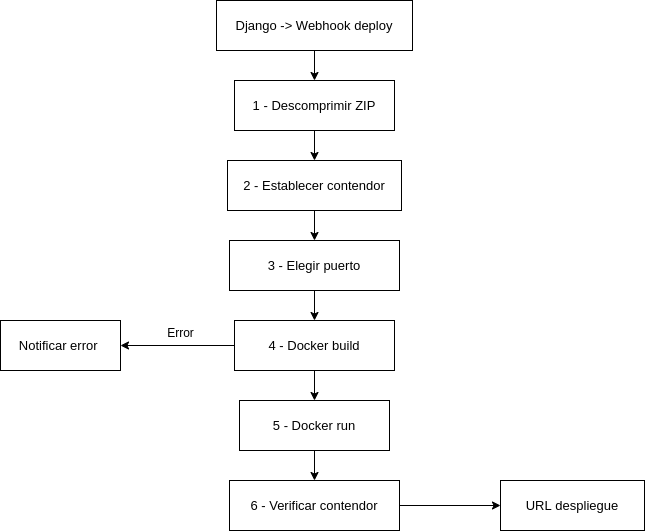
\includegraphics[width=0.5\textwidth]{img/disenoimplementacion/workflowdespliegue.png}
    \caption{Workflow de despliegue n8n}
    \label{fig:workflow-despliegue}
\end{figure}
\section{Sprint 5: Refactor del proyecto y consolidación del generador}
\label{sec:refactor-consolidacion-generador}

Una vez realizadas las primeras pruebas del generador, el código del fichero 
\textbf{project\_generator.py} había crecido considerablemente hasta convertirse 
en un módulo difícil de mantener y depurar. Esta situación causó un refactor 
profundo del proyecto, que no se limitó al generador sino que abarcó también 
los ficheros de presentación, el sistema de prompts y la trazabilidad de las 
llamadas al LLM.

Este sprint se dividió en dos bloques principales. En primer lugar, la 
refactorización del generador y de los ficheros de presentación, dividiendo 
el código en módulos más pequeños y mantenibles. En segundo lugar, la 
incorporación de nuevas funcionalidades de trazabilidad y análisis, como el 
modelo \textbf{GenerationLog}, el verificador de consistencia y el panel de 
métricas.

\subsection{Refactor del generador en módulos}
\label{subsec:refactor-generador-modulos}

Estos cambios fueron muy importantes, los pasos del generador se realizaban con 
todo el contenido dentro del mismo fichero, algo que no era de fácil escalabilidad 
a futuro, por lo que el primer cambio fue dividir el \textbf{project\_generator.py} 
en cuatro ficheros encargados cada uno de una labor especifica dentro de 
\textbf{utils/generator}, como se muestra en la Figura~\ref{fig:modulos-generador}.

\begin{figure}[H]
    \centering
    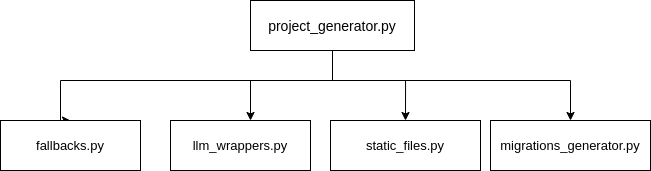
\includegraphics[width=0.8\textwidth]{img/disenoimplementacion/modulosgenerador}
    \caption{Estructura de módulos del generador tras el refactor}
    \label{fig:modulos-generador}
\end{figure}

\begin{itemize}
    \item \textbf{\texttt{llm\_wrappers.py}}: Centralizó todas las llamadas 
    al LLM en tres funciones reutilizables. \texttt{llm\_call} para llamadas 
    básicas que devuelven texto, \texttt{llm\_json\_call} para llamadas que 
    esperan JSON como respuesta, y \texttt{llm\_call\_logged} para llamadas 
    que además guardan un registro automático en base de datos con el prompt 
    enviado, la respuesta recibida y los posibles errores, a través del modelo 
    \textbf{GenerationLog} descrito en la 
    subsección~\ref{subsec:trazabilidad-generationlog}.

    \item \textbf{\texttt{fallbacks.py}}: Agrupó todos los fallbacks de 
    emergencia en un único fichero. Cada función de este módulo generaba una 
    versión mínima pero funcional de un artefacto concreto del proyecto: 
    páginas, modelos, vistas o templates. Al tenerlos centralizados resultaba 
    mucho más sencillo mejorarlos o ajustarlos sin tocar el orquestador principal.

    \item \textbf{\texttt{static\_files.py}}: Extrajo toda la generación de 
    ficheros de infraestructura que no dependen del LLM: \texttt{manage.py}, 
    \texttt{settings.py}, \texttt{wsgi.py}, \texttt{urls.py}, \texttt{Dockerfile}, 
    \texttt{entrypoint.sh} y \texttt{requirements.txt}. El orquestador principal 
    quedó así mucho más limpio, delegando en este módulo la construcción del 
    scaffolding fijo.

    \item \textbf{\texttt{migrations\_generator.py}}: Aisló la lógica de 
    generación automática de la migración inicial, que parseaba el 
    \texttt{models.py} producido por el LLM y construía el fichero 
    \texttt{0001\_initial.py} correspondiente.
\end{itemize}

\subsection{Refactor de templates y ficheros de estilos}
\label{subsec:refactor-templates-estilos}

La misma causa que creó la decisión del refactor del generador ocurrió con los ficheros de presentación del proyecto (HTML, CSS y JavaScript).
Hasta el momento los templates HTML eran ficheros que incluían todas las secciones en un único bloque, al igual que ocurría con los ficheros CSS y JavaScript. Como se mencionó anteriormente, este sprint introdujo una reorganización completa de la interfaz con la separación de responsabilidades.

En cuanto a los templates se creó un nuevo módulo \textbf{partials}, encargado de contener los fragmentos que representan una sección concreta de cada página. Cada fichero principal pasó a contener sus partials, incluyendose mediante la etiqueta \textbf{include} de Django.

La home del proyecto, que hasta entonces era el fichero más complejo, se dividió en seis partials independientes. En la Tabla~\ref{tab:partials-html} se muestra la estructura completa de partials tras el refactor:

\begin{table}[H]
    \centering
    \begin{tabular}{|l|l|p{5cm}|}
        \hline
        \textbf{Partial} & \textbf{Página} & \textbf{Responsabilidad} \\
        \hline
        hero.html & home & Sección principal de bienvenida \\
        \hline
        examples.html & home & Ejemplos de sitios generados \\
        \hline
        how.html & home & Explicación del funcionamiento \\
        \hline
        llms.html & home & Modelos de lenguaje compatibles \\
        \hline
        metrics.html & home & Métricas públicas del sistema \\
        \hline
        cta.html & home & Botón de acceso a la aplicación \\
        \hline
        input.html & assistant & Formulario de introducción de URL \\
        \hline
        analysis.html & assistant & Resultado del análisis del dataset \\
        \hline
        preview.html & assistant & Schema propuesto por la IA \\
        \hline
        published\_sites.html & history & Sitios generados y desplegados \\
        \hline
        recent\_analysis.html & history & Análisis recientes del usuario \\
        \hline
    \end{tabular}
    \caption{Partials HTML tras el refactor de templates}
    \label{tab:partials-html}
\end{table}

El asistente se dividió en tres partials dentro de \texttt{templates/WebBuilder/partials/assistant/}:

\begin{itemize}
    \item \texttt{input.html} — formulario del paso 1, donde el usuario 
    introduce la URL de la API o sube un fichero local para su análisis
    \item \texttt{analysis.html} — resultado del paso 2, que muestra las 
    estadísticas del dataset analizado: número de items encontrados, campos 
    disponibles y ruta de la colección principal
    \item \texttt{preview.html} — resultado del paso 3, donde se muestra 
    el schema propuesto por la IA y el usuario puede revisarlo y aprobarlo 
    antes de continuar
\end{itemize}

El historial se dividió en dos partials dentro de \texttt{templates/WebBuilder/partials/history/}:

\begin{itemize}
    \item \texttt{published\_sites.html} — listado de sitios ya generados 
    y desplegados por el usuario
    \item \texttt{recent\_analysis.html} — listado de análisis recientes 
    realizados por el usuario
\end{itemize}

Los ficheros estáticos sufrieron una reorganización equivalente. 
El CSS pasó a estar organizado por página y por sección dentro de \texttt{static/css/}, como se muestra en la Tabla~\ref{tab:ficheros-css}:


\begin{table}[H]
    \centering
    \begin{tabular}{|l|p{8cm}|}
        \hline
        \textbf{Fichero} & \textbf{Responsabilidad} \\
        \hline
        home/hero.css & Estilos de la sección principal de bienvenida \\
        \hline
        home/examples.css & Estilos de la sección de ejemplos \\
        \hline
        home/how.css & Estilos de la sección de funcionamiento \\
        \hline
        home/llms.css & Estilos de la sección de modelos compatibles \\
        \hline
        home/metrics.css & Estilos de la sección de métricas públicas \\
        \hline
        home/cta.css & Estilos de la sección de acceso \\
        \hline
        assistant.css & Estilos del asistente de generación \\
        \hline
        history.css & Estilos del historial del usuario \\
        \hline
        edit.css & Estilos de la página de edición del schema \\
        \hline
        login.css & Estilos de las páginas de login y registro \\
        \hline
        navbar.css & Estilos de la barra de navegación \\
        \hline
        backgrounds.css & Fondos y efectos visuales compartidos \\
        \hline
    \end{tabular}
    \caption{Ficheros CSS tras la reorganización de estilos}
    \label{tab:ficheros-css}
\end{table}

El JavaScript siguió el mismo criterio con ficheros independientes por página en \texttt{static/js/}, como se muestra en la Tabla~\ref{tab:ficheros-js}:

\begin{table}[H]
    \centering
    \begin{tabular}{|l|p{8cm}|}
        \hline
        \textbf{Fichero} & \textbf{Responsabilidad} \\
        \hline
        home.js & Lógica interactiva de la home \\
        \hline
        assistant.js & Lógica del flujo del asistente \\
        \hline
        edit.js & Lógica de la edición del schema \\
        \hline
        site\_render.js & Lógica de la vista previa del sitio generado \\
        \hline
    \end{tabular}
    \caption{Ficheros JavaScript tras la reorganización}
    \label{tab:ficheros-js}
\end{table}


El \texttt{base.html} se actualizó para cargar las fuentes de Google Fonts 
necesarias para el nuevo diseño: Inter para el texto general, 
y Geist y Geist Mono para elementos de código y datos técnicos.

Esta reorganización, aunque invisible para el usuario final, facilitó enormemente el mantenimiento y la evolución de la interfaz en los sprints siguientes, ya que cualquier cambio en una sección concreta de una página solo requería tocar un fichero pequeño y bien delimitado.

La Figura~\ref{fig:previewold} muestra el aspecto del asistente tras el 
refactor visual, donde se puede apreciar el nuevo layout de dos columnas, 
el esquema generado por la IA visible en tiempo real a la derecha, 
el selector de modelo LLM y los nuevos controles de idioma y tema.

\begin{figure}[H]
    \centering
    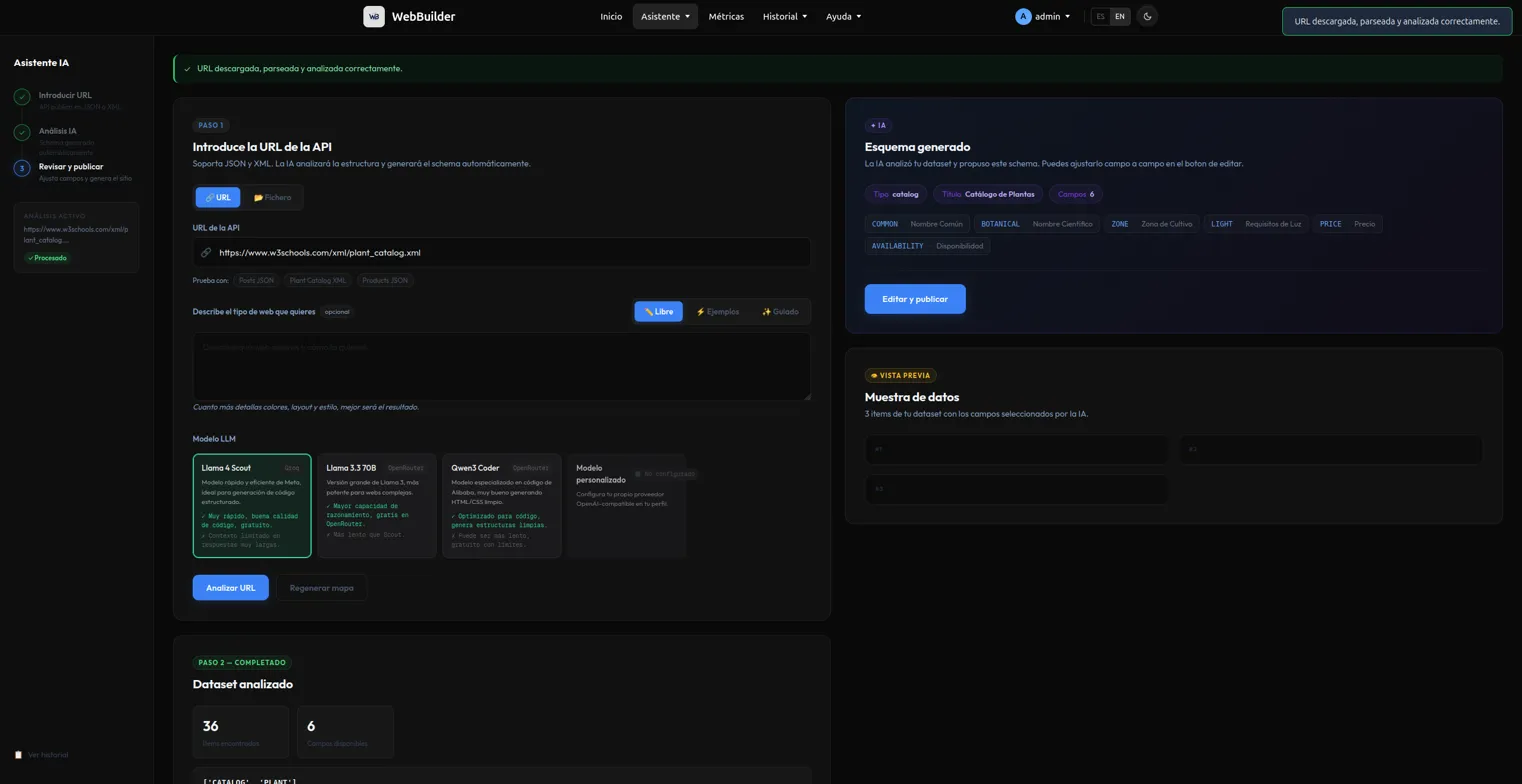
\includegraphics[width=\textwidth]{img/oldversions/previewold.png}
    \caption{Interfaz del asistente tras el refactor visual del Sprint 5}
    \label{fig:previewold}
\end{figure}

\subsection{Enriquecimiento de prompts}
\label{subsec:enriquecimiento-prompts}

Tras unas cuantas pruebas, se llegó a la conclusión de un problema importante, podría ocurrir que un usuario no familiarizado con los prompts de IA no supiese cómo hacerlo adecuadamente, o que incluso lo dejase vació. Para resolver este problema se creó el fichero \texttt{utils/llm/enrich\_prompts.py}, 
encargado de analizar automáticamente los campos del dataset antes de construir el prompt y añadir contenido personalizado.
Si el dataset tenía campos con imagenes se le indica al modelo que las usara de forma destacada. Si tenía precios, que los resalte visualmente. Si tenía
fechas que las mostrara de forma clara. De esta forma se garantiza que el LLM siempre recibiera suficiente contexto para tomar decisiones razonadas.
De todos modos si algo no estuviese en la mente del usuario, en el siguiente paso de editar el schema podría modificarlo añadiendo los campos necesarios o modificando los existentes.


\subsection{Trazabilidad: GenerationLog}
\label{subsec:trazabilidad-generationlog}

Anteriormente en las generaciones si algo fallaba no había forma de saber qué prompt se había enviado exactamente, qué había respondido el modelo ni si había habido reintentos. Para arreglar esto se creó el modelo \textbf{GenerationLog}, vinculado mediante una clave a su correspondiente \textbf{GeneratedSite}. 

Cada llamada al LLM durante la generación de un proyecto producía un registro que almacenaba el paso concreto que se estaba generando, el modelo de LLM utilizado, el prompt de sistema y el prompt de usuario enviados, la respuesta en crudo devuelta por el modelo, los errores de consistencia detectados y si la llamada había necesitado un reintento. Esto permitía analizar a posteriori qué pasos fallaban con más frecuencia, qué modelos producían mejores resultados y qué tipos de datasets generaban más inconsistencias.


\subsection{Verificación de consistencia}
\label{subsec:verificacion-consistencia}

Otro problema frecuente era que el LLM no tenía suficiente contexto entre ficheros, principal causa de las alucinaciones del LLM. Ocurria lo siguiente:
se definía un campo con un nombre en \textbf{models.py} y luego en los demás ficheros se referenciaba con ligeros cambios, provocando errores de ejecución.
Para detectar estos casos antes de que el usuario desplegase el proyecto, se implementó el fichero \texttt{utils/llm/consistency\_checker.py}.

Este fichero extraía mediante expresiones regulares los campos definidos en \texttt{models.py} y buscaba en los demas templates las referencias a esos campos. Cualquier referencia encontrada diferente que no correspondiera al campo real del modelo, se registraba como error de consistencia. 
Estos errores se guardaban en el campo \texttt{consistency\_errors} del modelo \texttt{GenerationLog} correspondiente, permitiendo identificar qué pasos producian mas inconsistencias y cómo se producían, para el consiguiente arreglo a futuro.


\subsection{Panel de métricas}
\label{subsec:panel-metricas}

Para tener un uso mas sencillo y accesible del contenido de GenerationLog se añadió una vista de métricas en \textbf{views/metrics.py}, accesible únicamente para usuarios con permisos de administrador. El objetivo de esta vista era tener visibilidad real sobre el comportamiento del generador, los fallos más recurrentes, qué modelos eran más óptimos para cada tipo de página, etc.

El panel mostraba las siguientes estadísticas agregadas:

\begin{itemize}
    \item \textbf{Resumen general}: número total de registros en \texttt{GenerationLog}, sitios generados y análisis realizados hasta la fecha.
    \item \textbf{Desglose por paso}: para cada uno de los siete pasos del generador, se mostraba el número de llamadas realizadas, cuántas habían necesitado reintento y la tasa de reintento resultante. Esto permitía identificar qué pasos eran más problemáticos y priorizar las mejoras.
    \item \textbf{Distribución por modelo}: agrupación de las llamadas por modelo de LLM utilizado, lo que facilitaba comparar el rendimiento de distintos proveedores cuando se probaban configuraciones diferentes.
\end{itemize}

Esta información resultó útil para mejorar los siguientes sprints y realizar los cambios adecuados. Los datos reales recogidos por este panel se analizan en detalle en la Sección~\ref{sec:metricas-sistema}.


\input{capitulos/disenoimplementacion/sprint6}
\section{Sprint 7: Pulido y cierre}
\label{sec:pulido-cierre}

Esta último sprint se dedicó a pulir el sistema en todos sus puntos débiles, que eran: mejorar la calidad visual de los sitios generados, consolidar la infraestructura de producción y completar los workflows de n8n que quedaban pendientes. Por infraestructura de producción se entienden los cambios que hacen que el proyecto sea útil fuera del entorno de desarrollo, como por ejemplo la migración a una base de datos más robusta como PostgreSQL para soportar accesos concurrentes de múltiples usuarios, la gestión automática de contenedores Docker activos o la monitorización diaria del sistema. Es decir, no se añadieron funcionalidades realmente nuevas, sino que se llevaron las existentes a un nivel de madurez adecuado para la entrega.


\subsection{Sistema de presets visuales}
\label{subsec:sistema-presets-visuales}

Uno de los principales problemas durante todo el desarrollo fue que los proyectos tendían a parecerse entre si visualmente, independiente del tipo de contenido de la API, del prompt del usuario y del sitio generado. Para resolverlo se creó el módulo \textbf{utils/llm/design}, organizado en tres ficheros con responsabilidades distintas. Estos ficheros eran presets.py, snippets.py y theme\_rules.py.

El fichero \texttt{presets.py} define un catálogo de estilos visuales completos y muy distintos entre sí. Cada preset describe la paleta de colores, el tipo de layout, la estética de los componentes y las palabras clave del prompt del usuario que deben activarlo. Los presets disponibles en este sprint se muestran en la Tabla~\ref{tab:presets-visuales}:

\begin{table}[H]
    \centering
    \begin{tabular}{|l|l|p{5cm}|}
        \hline
        \textbf{Preset} & \textbf{Estética} & \textbf{Palabras clave activadoras} \\
        \hline
        Neo Terminal & Cyberpunk, fondo negro, acento neón & Terminal, dark, gaming, futurista \\
        \hline
        Bento Pop & Rejilla asimétrica, colores vivos & Mosaico, asimétrico \\
        \hline
        Quiet Editorial & Tipografía protagonista, estética revista & Por defecto para blogs \\
        \hline
        Magazine Split & Gran imagen dividida, tipografía impactante & Por defecto para catálogos \\
        \hline
        Glass Orbit & Glassmorphism, fondos oscuros, traslúcidos & Por defecto para portfolios \\
        \hline
    \end{tabular}
    \caption{Presets visuales disponibles en el módulo de diseño}
    \label{tab:presets-visuales}
\end{table}

Cada tipo de sitio tiene asignado un preset por defecto que se aplica cuando el prompt del usuario no contiene ningún estilo descrito, garantizando que el resultado siempre tenga una identidad visual coherente con el tipo de contenido.

El fichero \texttt{snippets.py} complementa los presets con fragmentos de HTML concretos y válidos para cada estilo: cards, heros y filas de listado con las clases Tailwind exactas que corresponden a cada preset. Estos snippets se incluyen en los prompts de generación de templates como ejemplos de referencia visual, asegurando que el LLM produzca código coherente con el estilo elegido.

El fichero \texttt{theme\_rules.py} contiene clases base para contenedores, cards, botones, badges y tipografía, junto con reglas críticas de uso de color para evitar que el LLM genere clases Tailwind inválidas, como \texttt{bg-\#111111} en lugar de la sintaxis correcta \texttt{bg-[\#111111]}.

\subsection{Migración a PostgreSQL}
\label{subsec:migracion-postgresql}

Durante todo el desarrollo, WebBuilder había utilizado SQLite como base de datos, lo cual era suficiente para el entorno de desarrollo pero inadecuado para producción. En este sprint se realizó la migración a PostgreSQL, que ofrece mayor robustez, soporte para accesos concurrentes y mejor rendimiento con volúmenes de datos crecientes.

La configuración en \texttt{settings.py} se actualizó para leer los parámetros de conexión desde variables de entorno: nombre de la base de datos (\texttt{DB\_NAME}), usuario (\texttt{DB\_USER}), contraseña (\texttt{DB\_PASSWORD}), host (\texttt{DB\_HOST}) y puerto (\texttt{DB\_PORT}, por defecto \texttt{5432}). La configuración anterior de SQLite se migró a la nueva base de datos. Las migraciones existentes se aplicaron sobre la nueva base de datos, conservando los logs y métricas generados durante el desarrollo. Tras la migración, el esquema completo de la base de datos quedó de la siguiente manera:

\begin{figure}[H]
    \centering
    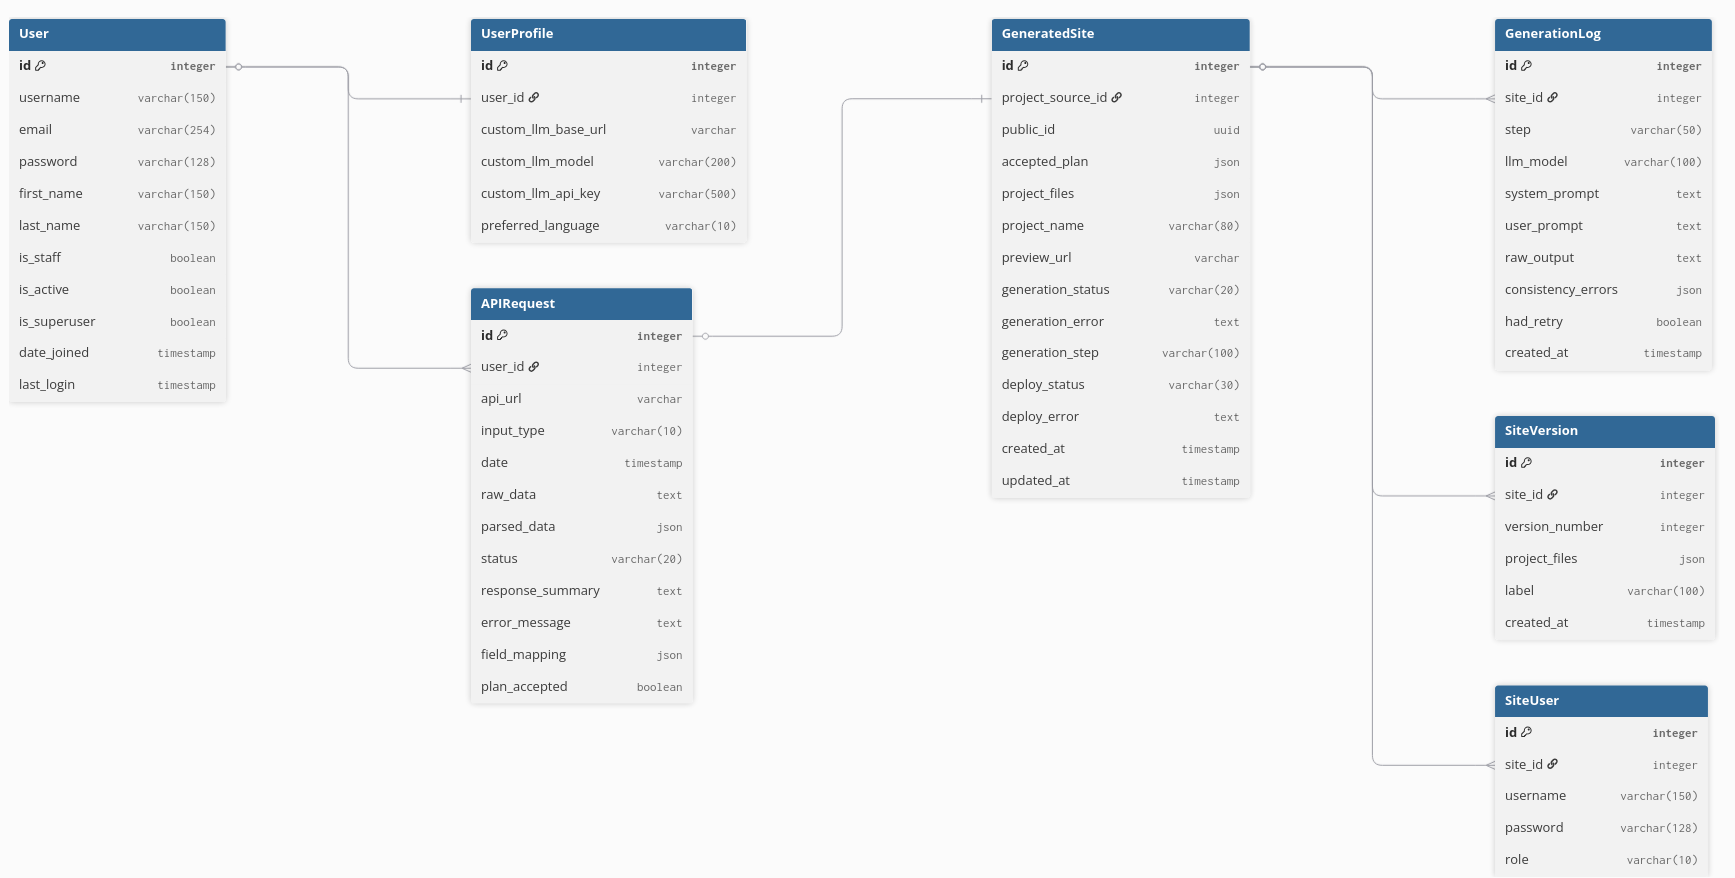
\includegraphics[width=\textwidth]{img/diagramaER.png}
    \caption{Esquema final de la base de datos}
    \label{fig:Esquema final de la base de datos}
\end{figure}


\subsection{Workflow generation-done}
\label{subsec:workflow-generation-done}

Con la base de notificaciones ya preparada desde el fichero \\ \texttt{utils/generator/notifications.py}, se implementó el workflow de n8n \emph{generation-done}. Este workflow se activa mediante un webhook al que Django llama en cuanto termina la generación de un sitio, enviando un payload con los datos relevantes: email y nombre del usuario, título y tipo del sitio generado, URL de la API original, URL del preview si ya está desplegado, URL de descarga del ZIP, número de campos e items procesados, duración de la generación en segundos y modelo de LLM utilizado.
n8n recibe este payload y envía automáticamente un correo de notificación al usuario informándole de que su sitio está listo. La llamada al webhook se realizó de forma completamente transparente al flujo principal: si n8n no estaba disponible o la llamada fallaba, la excepción se capturaba silenciosamente mediante un bloque \texttt{try/except} y la generación continuaba con normalidad.

\begin{figure}[H]
    \centering
    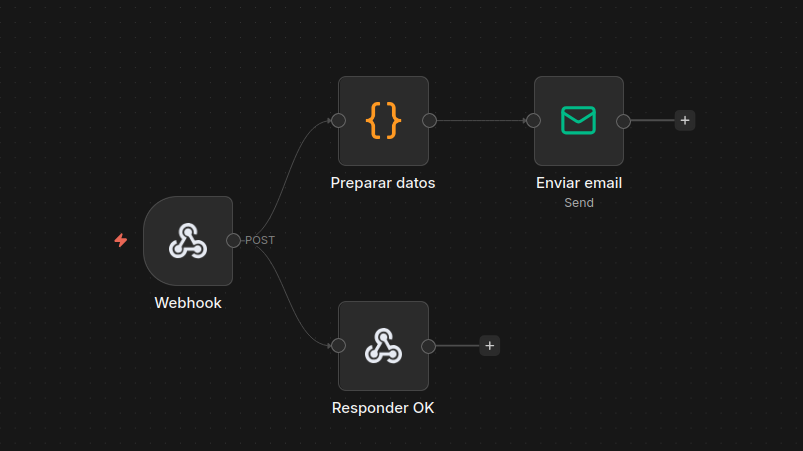
\includegraphics[width=0.7\textwidth]{img/n8n/generation-done.png}
    \caption{Workflow generation done}
    \label{fig:Workflow generation done}
\end{figure}

\subsection{Workflow health-check}
\label{subsec:workflow-health-check}

El workflow de \emph{health-check} se configuró para ejecutarse automáticamente cada día mediante un nodo \emph{Schedule Trigger} de n8n. Su función es verificar que el sistema sigue operativo realizando una petición HTTP a la URL principal de WebBuilder y comprobando que la respuesta es correcta. Si la verificación falla, n8n envía una alerta por correo al administrador del sistema con información sobre el error detectado. Aunque su uso fue puntual durante las últimas fases 
de desarrollo, ayudó a la monitorización del sistema para comprobar su correcto funcionamiento.

\begin{figure}[H]
    \centering
    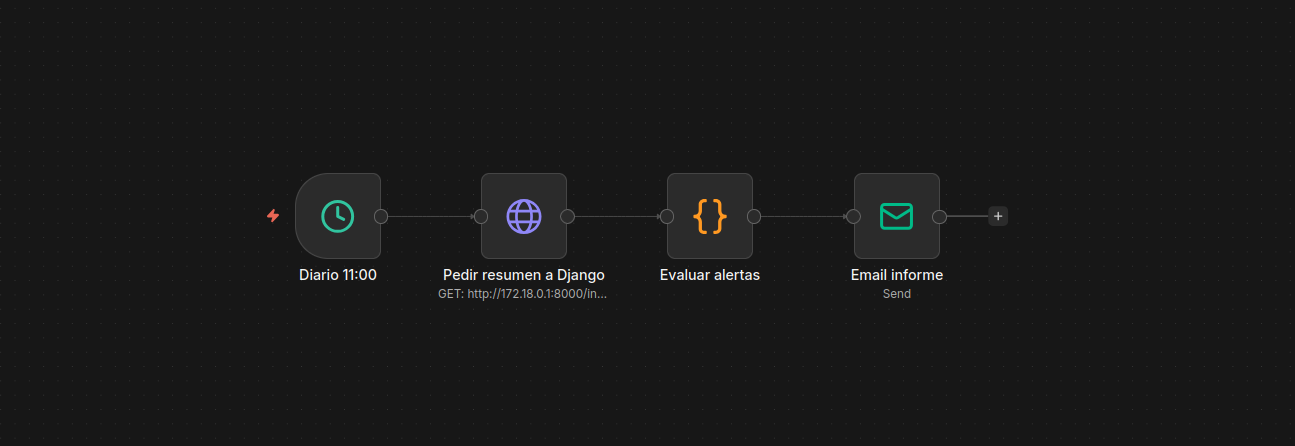
\includegraphics[width=\textwidth]{img/n8n/health-check.png}
    \caption{Workflow health check}
    \label{fig:Workflow health check}
\end{figure}


\subsection{Workflow auto-shutdown}
\label{subsec:workflow-auto-shutdown}

El workflow de \emph{auto-shutdown} resolvió un problema operativo importante: los contenedores Docker de los sitios generados permanecían activos indefinidamente aunque nadie los estuviera usando, consumiendo recursos del servidor. Este workflow se ejecuta de forma programada cada hora, consulta la lista de contenedores activos con el prefijo \texttt{wb\_} y detiene aquellos que están inactivos. Esto permite mantener el servidor limpio y los recursos disponibles para nuevas generaciones sin intervención manual.

\begin{figure}[H]
    \centering
    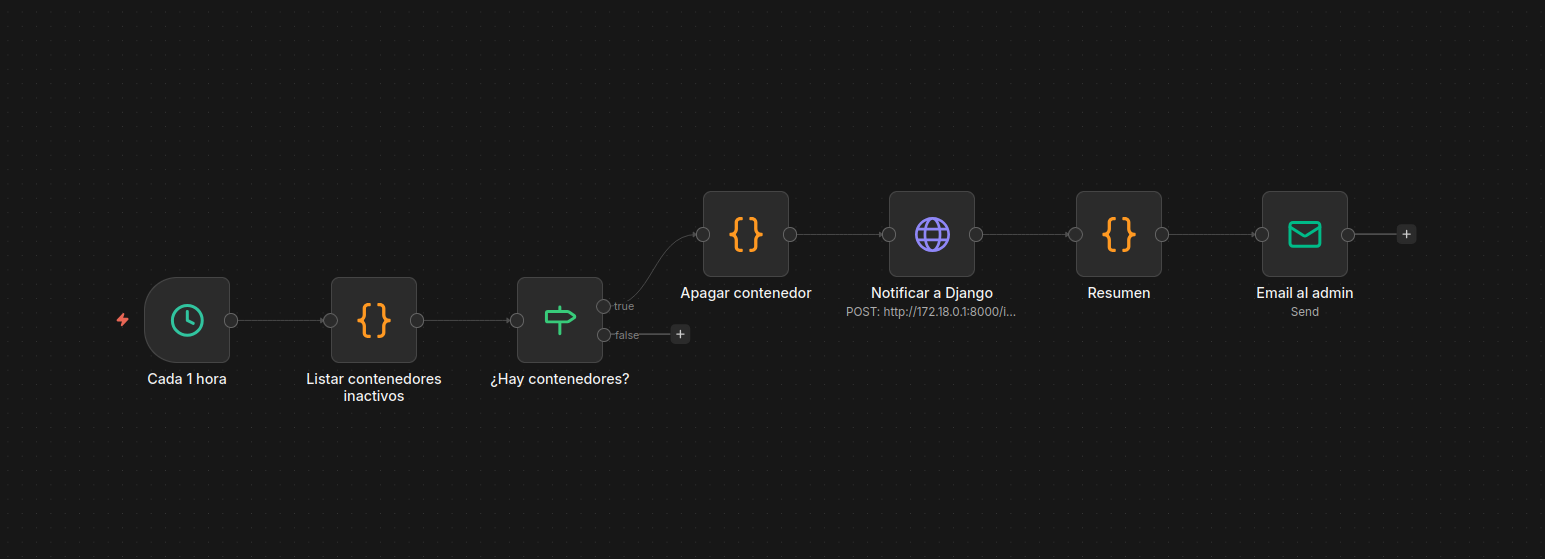
\includegraphics[width=\textwidth]{img/n8n/shutdown.png}
    \caption{Workflow auto shutdown}
    \label{fig:Workflow auto shutdown}
\end{figure}


\subsection{Mejora del workflow de despliegue}
\label{subsec:mejora-workflow-despliegue}

El workflow de despliegue que se había construido en el Sprint 4 carecía de un mecanismo centralizado de gestión de errores. Si cualquiera de los nodos fallaba, la petición de Django quedaba sin respuesta. En este sprint se añadió el nodo \textbf{Responder Error}, que actúa como rama de error compartida para todos los nodos del workflow. Cuando cualquier paso falla, este nodo captura el error y devuelve a Django una respuesta JSON estructurada con el código HTTP 500, un mensaje descriptivo del error y el paso en el que ocurrió. Esto permite que Django actualice el estado del sitio a \texttt{error} y muestre un mensaje útil al usuario, anteriormente se notificaba el error, pero no en detalle.

\begin{figure}[H]
    \centering
    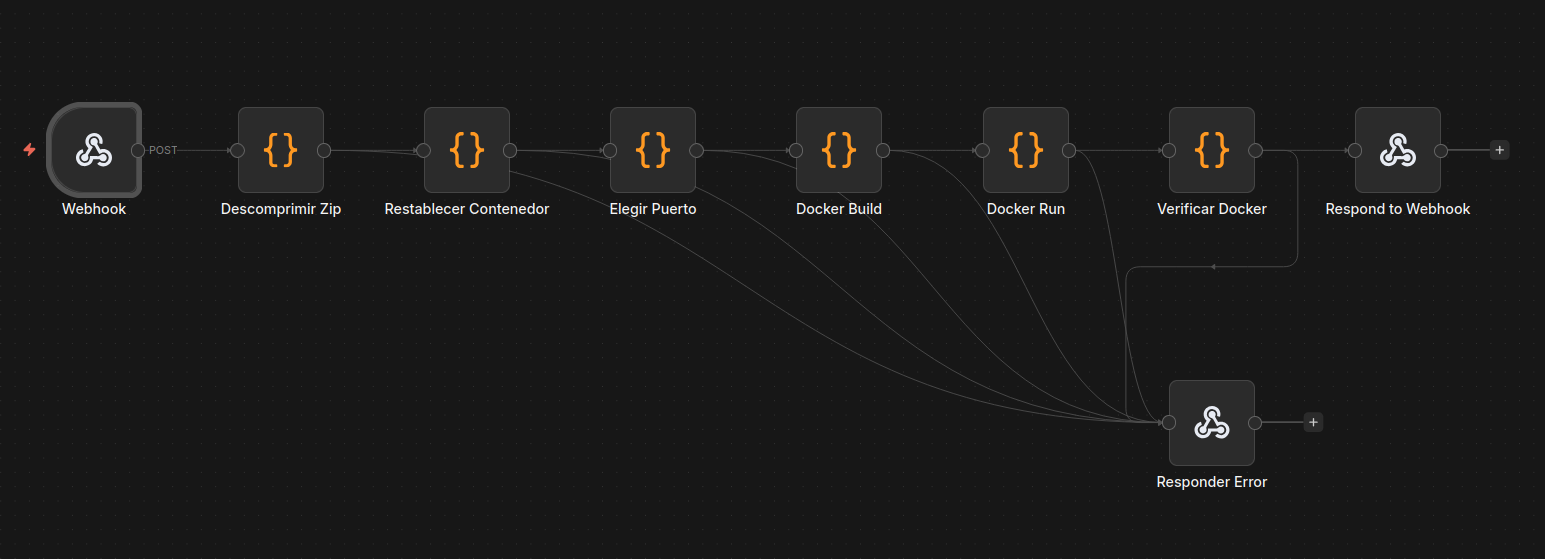
\includegraphics[width=\textwidth]{img/n8n/deploy.png}
    \caption{Workflow deploy}
    \label{fig:Workflow deploy}
\end{figure}


\subsection{Autenticación OAuth con Google y GitHub}
\label{subsec:oauth}

Antes del cierre del proyecto, se integró la autenticación mediante OAuth con Google y GitHub, permitiendo al usuario iniciar sesión o registrarse en WebBuilder con una cuenta ya creada. La autenticación se realizó con la librería \texttt{django-allauth}, que gestiona el flujo OAuth completo y se integra con el sistema de autenticación de Django que ya existía.

\subsubsection{Obtención de credenciales}
Para habilitar el login con Google fue necesario acceder a \textbf{Google Cloud Console}, crear un proyecto OAuth, configurar la pantalla de consentimiento y generar un par de credenciales \texttt{client\_id} y \texttt{client\_secret}. En la configuración del cliente se declaró la URL de redirección, que debe coincidir exactamente con la que allauth espera recibir, es la dirección encargada de devolverte a WebBuilder ya logueado:

\begin{center}
    \texttt{http://\textless{}dominio\textgreater{}/accounts/google/login/callback/}
\end{center}

Para GitHub el proceso es similar, en este caso a través de \textbf{GitHub Developer Settings, OAuth Apps}, donde también se declara la \emph{Authorization callback URL}.

Las credenciales obtenidas se añadieron al fichero \texttt{.env} del servidor como variables de entorno (\texttt{GOOGLE\_CLIENT\_ID}, \texttt{GOOGLE\_CLIENT\_SECRET}, \texttt{GITHUB\_CLIENT\_ID}, \\ \texttt{GITHUB\_CLIENT\_SECRET}) y se leen desde \texttt{settings.py}.


\subsubsection{Arquitectura de la integración}
La integración se compone de tres elementos principales:

\begin{itemize}
    \item \textbf{Adaptador OAuth} (\texttt{WebBuilder/adapters.py}): adaptador personalizado que sobreescribe el comportamiento por defecto de allauth en tres métodos. \texttt{save\_user()} se ejecuta únicamente la primera vez que un usuario accede con OAuth, es decir, en el momento del registro, y dispara el webhook de n8n correspondiente. \texttt{pre\_social\_login()} se ejecuta en cada acceso posterior y dispara el webhook de login con datos del acceso: IP, dispositivo y hora. Por último, \texttt{on\_authentication\_error()} captura cualquier error del flujo OAuth, lo registra en los logs y redirige al usuario a la página de login, evitando que allauth muestre su página de error por defecto sin estilos.

    \item \textbf{Signal \texttt{post\_save}} (\texttt{WebBuilder/signals.py}): garantiza que se cree un \\ \texttt{UserProfile} vacío para cualquier usuario nuevo, independientemente de si se registró mediante el formulario tradicional o mediante OAuth.

    \item \textbf{Templates de allauth} (\texttt{WebBuilder/templates/socialaccount/}): allauth dispone de sus propias páginas HTML para los flujos de autenticación social; cuando no encuentra un template personalizado utiliza los suyos propios, que carecen de estilos. Se crearon templates propios para \texttt{login.html}, \texttt{signup.html} y \\ \texttt{authentication\_error.html} respetando el sistema de estilos del proyecto.
\end{itemize}


\subsubsection{Problemas encontrados durante la puesta en producción}
La integración resultó más compleja de lo esperado por la acumulación de varios problemas independientes que se manifestaban de la misma manera: \emph{Third-Party Login Failure}.

El primer problema fue que la \texttt{SECRET\_KEY} de Django no estaba definida en el \texttt{.env} de producción, por lo que el sistema generaba una clave aleatoria en cada arranque del contenedor. Esto invalidaba las sesiones activas, lo que rompía el flujo OAuth: allauth guarda el parámetro \texttt{state} en la sesión antes de redirigir al proveedor, y si el contenedor se reiniciaba entre la redirección y el callback, la sesión no podía verificarse. La solución fue generar una clave fija y añadirla al \texttt{.env}.

El segundo problema fue el framework \texttt{django.contrib.sites}, que allauth utiliza para construir las URLs de callback, tenía en base de datos el dominio por defecto \texttt{example.com} en lugar del dominio real del servidor. La solución fue editar el registro en el panel de administración de Django (\texttt{/admin/sites/site/}) con el dominio correcto.

El tercer problema fue que las variables \texttt{ALLOWED\_HOSTS} y \texttt{CSRF\_TRUSTED\_ORIGINS} no estaban en el \texttt{.env} de producción pero sí en el local, lo que provocaba que Django rechazara las peticiones del proveedor OAuth. Se añadieron en producción con el dominio del servidor. 

Una vez resueltos todos estos problemas, el flujo OAuth funciona de extremo a extremo: el usuario hace clic en \emph{Login con Google} o \emph{Login con GitHub}, es redirigido al proveedor, selecciona su cuenta y regresa a WebBuilder ya autenticado, con su perfil creado automáticamente y los webhooks de n8n notificados.


\begin{figure}[H]
    \centering
    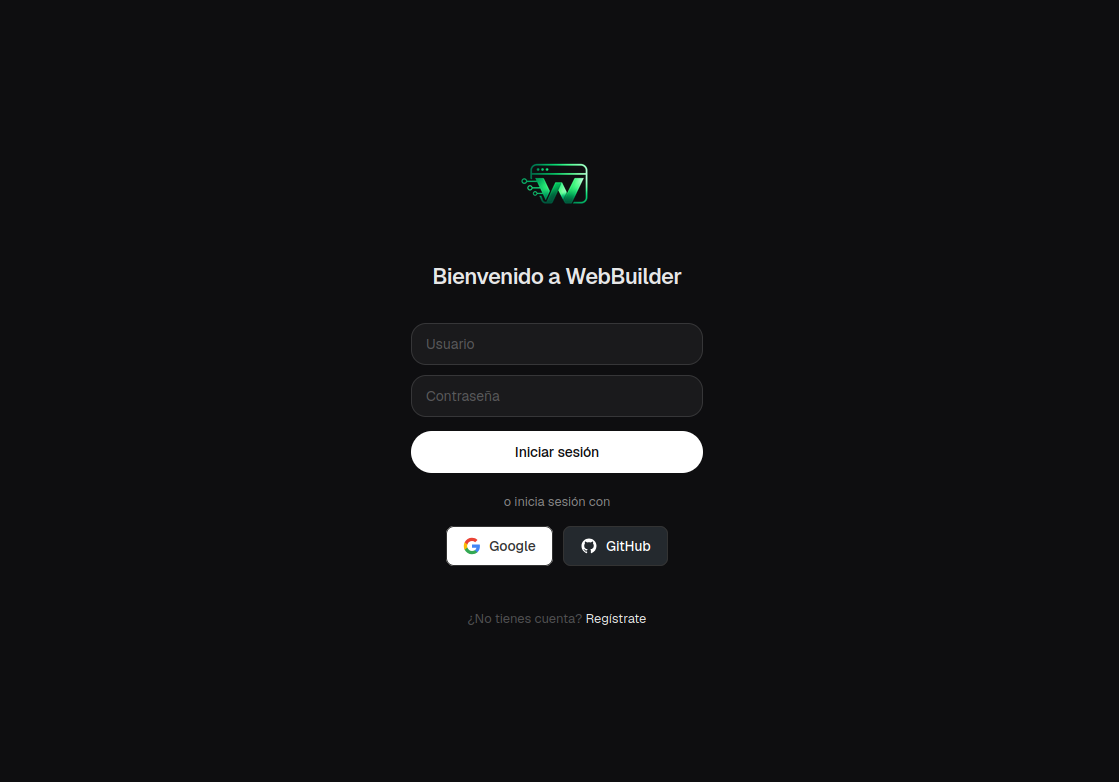
\includegraphics[width=0.9\textwidth]{img/webbuilder/disenoimplementacion/oauth.png}
    \caption{Autenticación Oauth}
    \label{fig:Autenticación Oauth}
\end{figure}

%%%%%%%%%%%%%%%%%%%%%%%%%%%%%%%%%%%%%%%%%%%%%%%%%%%%%%%%%%%%%%%%%%%%%%%%%%%%%%%%
%%%%%%%%%%%%%%%%%%%%%%%%%%%%%%%%%%%%%%%%%%%%%%%%%%%%%%%%%%%%%%%%%%%%%%%%%%%%%%%%
% EXPERIMENTOS Y VALIDACIÓN %
% Resultado del TFG - app web, manual de usuario, test, experimentos, etc%
%%%%%%%%%%%%%%%%%%%%%%%%%%%%%%%%%%%%%%%%%%%%%%%%%%%%%%%%%%%%%%%%%%%%%%%%%%%%%%%%

\cleardoublepage
\chapter{Experimentos y validación}
\label{chap:experimentos}

%Este capítulo se introdujo como requisito en 2019. 
%Describe los experimentos y casos de test que tuviste que implementar para validar tus resultados. 
%Incluye también los resultados de validación que permiten afirmar que tus resultados son correctos. 

\subsection{Metodoloǵia de validación}
\label{subsec:metodologia-validacion}

La validación de WebBuilder se ha llevado a cabo mediante la generación de casos de uso reales, utilizando APIs públicas de distinta naturaleza y complejidad. El objetivo no ha sido medir la perfección de un resultado concreto, sino evaluar la capacidad del sistema para producir proyectos Django funcionales, desplegables y visualmente coherentes a partir de cualquier fuente de datos.

Para cada caso de uso se han evaluado los siguientes criterios:

\begin{itemize}
	\item \textbf{Funcionalidad:} el proyecto generado arranca correctamente, carga los datos de la API y las páginas responden sin errores HTTP.
	
	\item \textbf{Coherencia del modelo de datos:} los campos detectados por el sistema corresponden a los datos reales de la API y el modelo Django generado los representa correctamente.
	
	\item \textbf{Calidad del código generado:} el código producido por el LLM es sintácticamente correcto, no contiene campos inexistentes y supera la verificación de consistencia del sistema.
	
	\item \textbf{Calidad visual:} el sitio generado tiene una apariencia coherente con el tipo de contenido, los presets visuales se aplican correctamente y la navegación entre páginas funciona.
	
	\item \textbf{Despliegue automático:} el workflow de n8n completa el proceso de build y arranque del contenedor Docker sin intervención manual, devolviendo una URL de previsualización accesible.
\end{itemize}

Además de los casos de uso, se ha realizado un análisis de los errores ocurridos en el proceso de desarrollo, categorizados por tipo y documentados con su causa, consecuencia y solución aplicada, que se recoge en la Sección~\ref{sec:analisis-errores}.


\subsection{Casos de uso}
\label{subsec:casos-uso}

\subsection{Análisis de errores}
\label{subsec:analisis-errores}

Durante el proceso de desarrollo y pruebas de WebBuilder se identificaron y documentaron de forma sistemática los principales errores que afectaban a la calidad de las generaciones. Estos errores se agrupan en dos categorías: limitaciones impuestas por los propios modelos de lenguaje y errores en el código generado por el LLM.

\subsubsection{Errores de limitación del LLM}
\label{subsubsec:errores-llm}

La primera categoría de errores está relacionada con los límites de uso de los proveedores de modelos, que condicionan directamente el comportamiento del sistema durante la generación.


\textbf{Error HTTP 429 — Rate Limit Exceeded.} El error más frecuente durante las pruebas fue la superación del límite de tokens por minuto del modelo. El prompt del paso de generación de templates es especialmente grande, ya que incluye el prompt enriquecido, los campos del modelo, los datos de ejemplo y un fragmento HTML de referencia. Cuando este prompt superaba los tokens disponibles en el minuto en curso, la llamada fallaba y el template afectado caía al fallback vacío, generando una página en blanco. La solución aplicada fue reducir el tamaño máximo del prompt enriquecido, eliminar los datos de ejemplo del paso de estructura de páginas y truncar el ejemplo HTML de referencia a 1500 caracteres.

\textbf{Error HTTP 413 — Request Entity Too Large.} Algunos modelos como \texttt{groq/compound} rechazan peticiones que superan un cierto tamaño en bytes antes de procesarlas, independientemente del límite de TPM. Este error afectaba prácticamente a todos los pasos de la generación, dejando el proyecto resultante vacío o lleno de fallbacks. La solución fue descartar este modelo del catálogo recomendado y sustituirlo por \texttt{meta-llama/llama-4-scout-17b-16e-instruct}, que ofrece 30K TPM sin restricciones de tamaño de petición.

\textbf{Timeout por \texttt{time.sleep} excesivo.} Durante las pruebas se intentó evitar el error 429 aumentando el tiempo de espera entre llamadas al LLM hasta 60 segundos. El resultado fue que el servidor web cortaba la conexión por timeout antes de que terminara la generación. La conclusión fue que el sleep no debe superar los 20 segundos y que la solución correcta al problema de TPM es reducir el tamaño de los prompts, no aumentar la espera entre llamadas.


En la Tabla~\ref{tab:modelos-groq} se recoge la comparativa de modelos evaluados en Groq durante las pruebas, con sus límites y observaciones:

\begin{table}[H]
	\centering
	\begin{tabular}{|p{6cm}|l|l|p{4cm}|}
	\hline
	\textbf{Modelo} & \textbf{TPM} & \textbf{RPD} & \textbf{Observaciones} \\
	\hline
	\texttt{groq/compound} & 70K & Sin límite & Límite de tamaño de request muy restrictivo. No recomendado. \\
	\hline
	\texttt{openai/gpt-oss-120b} & 8K & 200K & Buena calidad pero TPM muy bajo. Falla en prompts grandes. \\
	\hline
	\texttt{llama-3.3-70b-versatile} & 12K & 100K & Aceptable pero con menos margen. \\
	\hline
	\texttt{llama-4-scout-17b-16e} & 30K & 500K & Recomendado. Buen equilibrio calidad/límites. \\
	\hline
\end{tabular}
\caption{Comparativa de modelos evaluados en Groq}
\label{tab:modelos-groq}
\end{table}


\subsubsection{Errores en el código generado}
\label{subsubsec:errores-codigo}


\subsection{Errores en el código generado}
\label{subsec:errores-codigo}

La segunda categoría agrupa los errores producidos por el propio LLM al generar el código del proyecto, independientemente de los límites del proveedor.

\textbf{Acceso a subcampos de objetos anidados.} Cuando el dataset contiene campos que son objetos anidados, como \texttt{origin: {name: Earth'', url: ...''}}, el LLM tiende a tratarlos como objetos Django en el template usando la sintaxis \texttt{{{ item.origin.name }}}. Sin embargo, el modelo Django almacena ese campo como un \texttt{CharField} simple con solo el valor del nombre. El resultado es un error en tiempo de ejecución al intentar acceder a \texttt{.name} sobre un string. Este error es especialmente difícil de detectar automáticamente porque el verificador de consistencia solo comprueba que el primer nivel de campo exista en el modelo.

\textbf{URLs hardcodeadas incorrectas en templates.} El LLM tiende a usar nombres de URL genéricos como \texttt{detail} o \texttt{catalog} en las etiquetas \texttt{url} aunque el prompt le indique los nombres exactos. Esto provoca errores \texttt{NoReverseMatch} en tiempo de ejecución. La solución aplicada fue añadir una validación en \texttt{check\_django\_syntax} que comprueba que todos los nombres de URL usados en los templates corresponden a URLs reales del proyecto.

\textbf{\texttt{json.loads} sobre un dict ya parseado.} Cuando el dataset tiene campos anidados, el LLM a veces genera en \texttt{load\_data.py} llamadas a \texttt{json.loads()} sobre campos que ya han sido deserializados por \texttt{response.json()}. El resultado es un \texttt{json.JSONDecodeError} que hace que todos los items fallen silenciosamente y no se cargue ningún dato en la base de datos.

\textbf{Variables de contexto inconsistentes entre view y template.} En ocasiones el LLM usa nombres semánticamente descriptivos en la view, como \texttt{featured} o \texttt{recent}, en lugar del nombre estándar \texttt{items} que usan los templates. El resultado es que la página aparece vacía aunque haya datos en la base de datos. La solución fue reforzar en los prompts de generación que la variable del contexto debe llamarse siempre \texttt{items}.

\textbf{Paginación no implementada en APIs paginadas.} Cuando la API devuelve los datos paginados, el \texttt{load\_data.py} generado por defecto solo hace una petición a la URL base, cargando únicamente la primera página de resultados. Esto puede suponer cargar 20 items de una API que tiene 800, sin que el sistema lo detecte como un error.


\section{Métricas del sistema}
\label{sec:metricas-sistema}

WebBuilder incorpora un panel de métricas accesible unicamente para administradores que recopila datos en tiempo real sobre el funcionamiento del sistema. Esta sección presenta los resultados extraídos del panel tras el uso de la pagina, que permiten evaluar de forma objetiva tanto el rendimiento como la fiabilidad de la plataforma.

El panel se estructura en seis vistas independientes (Resumen, Actividad, LLM, Alertas, Usuarios y Generaciones), cada una enfocada en un aspecto distinto del sistema. Tanto los datos numéricos como las capturas que se muestran a continuación corresponden a una instantánea del sistema en el momento de redactar esta memoria, por lo que pueden no coincidir exactamente con los valores actuales en el momento de la lectura.

\subsection{Resumen general}
\label{subsec:metricas-resumen}

El sistema acumula 67 análisis de APIs realizados, de los cuales 61 han sido generados con éxito. Esto supone una tasa de éxito del análisis del 95.5\% y una conversión análisis-a-sitio del 91\%, lo que indica que el flujo completo desde la ingesta de datos hasta la generación final es estable y fiable. La tasa de reintentos del LLM se mantiene en el 0\%, dentro del rango esperado para los modelos seleccionados como recomendados tras los ajustes descritos en la Sección~\ref{subsec:errores-llm}.

\subsection{Actividad y patrones de uso}
\label{subsec:metricas-actividad}

El panel de actividad muestra la evolución de los análisis y las generaciones en los últimos 30 días. Se observan picos de uso en los periodos de desarrollo de mejora de visualizacion, alcanzando hasta 15 análisis en un mismo.

En cuanto a los formatos de entrada utilizados, el 95\% de los análisis se han realizado a partir de URLs de APIs públicas, siendo el 5\% restante análisis de ficheros locales.

La distribución de llamadas al LLM depende del tipo de ficheros: los pasos de generación de templates, modelos, carga de datos, vistas y plantilla base concentran 56 llamadas cada uno, mientras que los templates específicos de catálogo y detalle bajan a 26 y 23 respectivamente. 

Esto se debe a que estos últimos solo se generan cuando el tipo de sitio elegido los requiere, mientras que los anteriores son comunes a cualquier proyecto generado.

\subsection{Rendimiento de los modelos LLM}
\label{subsec:metricas-llm}

El sistema acumula 456 llamadas totales al LLM, repartidas entre los cuatro modelos evaluados. La distribución refleja claramente las decisiones tomadas durante el desarrollo:

\begin{itemize}
	\item \texttt{meta-llama/llama-4-scout-17b-16e-instruct}: 370 llamadas (81.1\%)
	\item \texttt{llama-3.3-70b-versatile}: 61 llamadas (13.4\%)
	\item \texttt{groq/compound-mini}: 16 llamadas (3.5\%)
	\item \texttt{groq/compound}: 9 llamadas (1.9\%)
\end{itemize}

El modelo \texttt{llama-4-scout} acumula la inmensa mayoría de las llamadas tras ser el modelo mas adecuado por su equilibrio entre calidad y límites de TPM, mientras que \texttt{groq/compound} fue descartado tras detectar el problema de tamaño máximo de petición. 

La tasa de errores de consistencia es del 0\% en todos los modelos, lo que valida la eficacia del sistema de verificación de código generado descrito en la Sección~\ref{subsec:errores-codigo}.

El número medio de llamadas por sitio generado es de 7.5, coherente con los 7 pasos del generador más alguna llamada adicional de validación.

\subsection{Alertas y estabilidad}
\label{subsec:metricas-alertas}

El panel de alertas detecta incidencias del sistema como generaciones bloqueadas, análisis pendientes o errores recientes. En el momento de la captura no había alertas activas ni errores registrados en las últimas 24 horas.

\subsection{Usuarios y proyectos generados}
\label{subsec:metricas-usuarios}

La plataforma cuenta con 4 usuarios registrados, todos ellos con al menos un sitio generado. La distribución de actividad muestra que el usuario \texttt{admin} concentra 52 análisis y 47 sitios generados (lo esperable dado que es la cuenta de pruebas principal), seguido por \texttt{Alejandro} con 9 análisis y 9 sitios, y los usuarios \texttt{Pruebasn8n} y \texttt{pruebas2} con volúmenes menores asociados a pruebas específicas.

El panel de generaciones muestra el listado completo de proyectos creados con su estado, nombre, usuario propietario, número de ficheros y antigüedad. Todos los proyectos listados se encuentran en estado \emph{ready}, lo que indica que su contenedor Docker está disponible y accesible mediante su URL de previsualización.
\cleardoublepage
\chapter{Resultados}
\label{chap:resultados}

Este capítulo recoge los resultados obtenidos tras el desarrollo y validación de WebBuilder, presentando el sistema como producto terminado y resumiendo las funcionalidades conseguidas.

\section{WebBuilder como plataforma}
\label{sec:webbuilder-plataforma}

Al finalizar el desarrollo de WebBuilder se han implementado y validado con éxito las siguientes funcionalidades:

\begin{itemize}
    \item Análisis automático de APIs públicas en los formatos JSON, XML, CSV y GeoJSON, con detección del esquema de datos mediante LLM y validación anti-alucinaciones.
    \item Generación completa de proyectos Django funcionales en siete pasos coordinados por el LLM, incluyendo modelos, vistas, plantillas, carga de datos y configuración de despliegue.
    \item Despliegue automático de los proyectos generados en contenedores Docker independientes mediante flujos de trabajo en n8n, devolviendo una URL de previsualización al usuario.
    \item Soporte para múltiples proveedores de modelos de lenguaje mediante el estándar OpenAI-compatible, con un catálogo de modelos preconfigurados y la posibilidad de conectar un proveedor personalizado.
    \item Sistema de trazabilidad completo con registro de cada llamada al LLM, verificación de consistencia del código generado y panel de métricas para administradores.
    \item Historial de versiones por proyecto, con posibilidad de redesplegar cualquier versión anterior, descargar el código fuente y refinar el sitio con el asistente de IA.
    \item Interfaz bilingüe (español e inglés) con modo claro y oscuro, accesible desde cualquier navegador sin instalación de software adicional.
\end{itemize}

\begin{figure}[H]
    \centering
    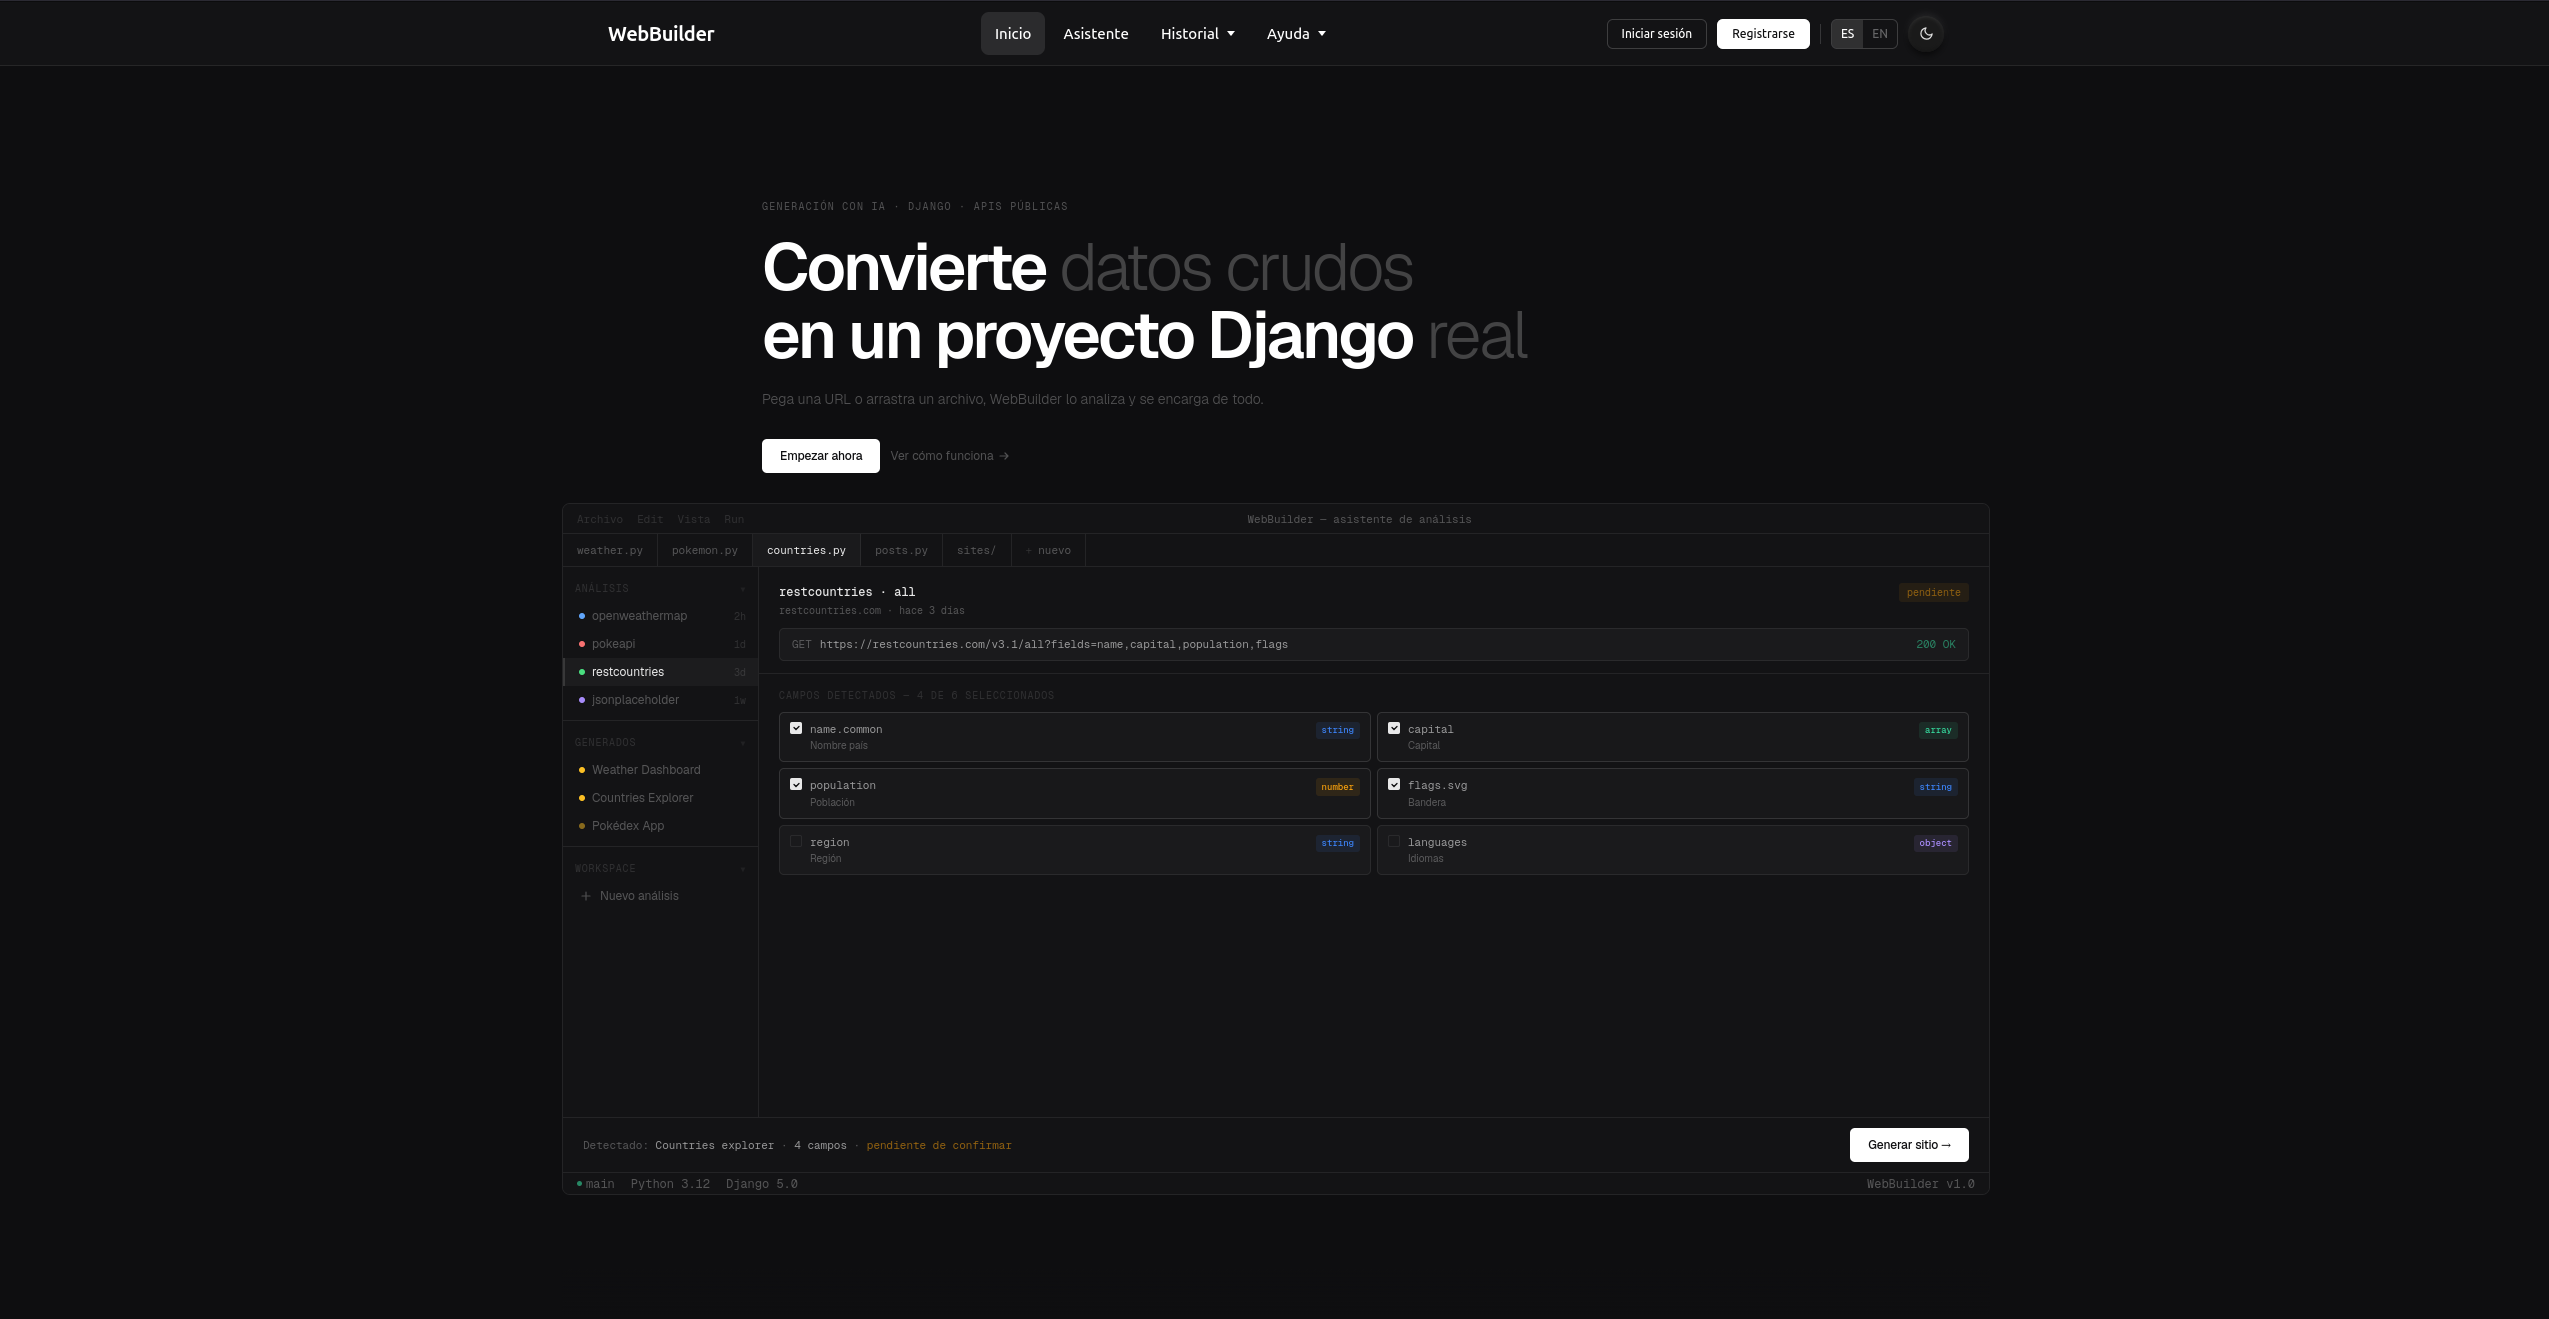
\includegraphics[width=\textwidth]{img/webbuilder/hero.png}
    \caption{Página principal de WebBuilder}
    \label{fig:wb-home}
\end{figure}

\section{Resultados casos de uso}
\label{sec:casos-uso-resultados}

Como demostración del funcionamiento real del sistema, se generaron tres sitios web completos a partir de APIs públicas de distinta naturaleza, cuyos resultados se describen en detalle en el Capítulo~\ref{chap:experimentos}. Los tres proyectos fueron generados de forma automática, desplegados en contenedores Docker independientes y validados según los criterios definidos en la metodología de validación.

El primer caso utilizó la API de TheCocktailDB para generar una web de recetas de cócteles con catálogo visual paginado y páginas de detalle. El segundo caso utilizó la API de SampleAPIs para generar un catálogo de películas de animación con pósters e información de cada título. El tercer caso utilizó la API de Rick and Morty para generar un catálogo de personajes con imágenes, badges de estado y páginas de detalle estructuradas.

Los tres casos demuestran que WebBuilder es capaz de adaptarse a tipos de datos y estilos visuales completamente distintos sin ninguna configuración adicional más allá del prompt inicial del usuario.

\section{Disponibilidad del software}
\label{sec:disponibilidad}

El código fuente de WebBuilder está disponible públicamente en el 
siguiente repositorio de GitHub:

\begin{center}
\url{https://github.com/AlejandroTejero/WebBuilder-TFG}
\end{center}

El proyecto se distribuye bajo la licencia \textbf{CC0 1.0 Universal} 
(\emph{Creative Commons Zero}), la cual equivale a subir el proyecto a dominio público. Esto 
significa que cualquier persona puede usar, modificar, distribuir o 
incorporar el código en el proyecto, sin necesidad de solicitar permiso al autor original. Contribuyendo de esta forma al ecosistema de aplicaciones de código abierto.

La landing page del proyecto, que actúa como página informativa y de documentación, 
se encuentra en el Apéndice~\ref{app:manual}.
%%%%%%%%%%%%%%%%%%%%%%%%%%%%%%%%%%%%%%%%%%%%%%%%%%%%%%%%%%%%%%%%%%%%%%%%%%%%%%%%
%%%%%%%%%%%%%%%%%%%%%%%%%%%%%%%%%%%%%%%%%%%%%%%%%%%%%%%%%%%%%%%%%%%%%%%%%%%%%%%%
% CONCLUSIONES %
%%%%%%%%%%%%%%%%%%%%%%%%%%%%%%%%%%%%%%%%%%%%%%%%%%%%%%%%%%%%%%%%%%%%%%%%%%%%%%%%

\cleardoublepage
\chapter{Conclusiones}
\label{chap:conclusiones}

En este capítulo se recogen las conclusiones obtenidas tras el desarrollo de WebBuilder. En primer lugar se evalúan los objetivos planteados al inicio del proyecto, analizando qué se ha logrado y qué limitaciones se han encontrado. A continuación se reflexiona sobre la aplicación de los conocimientos adquiridos durante el grado y las lecciones aprendidas a lo largo del desarrollo. Por último se proponen posibles líneas de trabajo futuro que podrían ampliar o mejorar el sistema en próximas iteraciones.

\section{Consecución de objetivos}
\label{sec:consecucion-objetivos}

%Y si has llegado hasta aquí, siempre es bueno pasarle el corrector ortográfico, que las erratas quedan fatal en la memoria final. Para eso, en Linux tenemos aspell, que se ejecuta de la siguiente manera desde la línea de \emph{shell}:
%
%\begin{verbatim}
%  aspell --lang=es_ES -c memoria.tex
%\end{verbatim}

Cabe destacar que una de las principales limitaciones encontradas durante el desarrollo ha sido la calidad visual de los sitios generados. La calidad que producen modelos de pago de alto rendimiento como GPT-4 o Claude no es alcanzable con los modelos gratuitos disponibles en los proveedores utilizados, y por más refinamiento aplicado en los prompts y en el sistema de presets visuales, llegar a ese nivel de calidad resulta prácticamente imposible sin acceso a modelos más potentes. Los objetivos marcados y conseguidos son los siguientes: 

\begin{itemize}
  \item \textbf{Desarrollar un módulo de ingestión de datos.} El módulo implementado en \\ \texttt{utils/ingest/} es capaz de validar la URL introducida por el usuario, descargar el contenido de la API de forma segura y detectar automáticamente el formato de los datos. Los cuatro formatos contemplados en el objetivo, JSON, XML, CSV y GeoJSON, están soportados y producen una estructura Python homogénea que el resto del sistema consume.
  
  \item \textbf{Integrar modelos de lenguaje para el análisis y la generación de código.} El módulo \texttt{utils/llm/} implementa un cliente compatible con el estándar OpenAI que permite conectar con cualquier proveedor del mercado. Los modelos de lenguaje intervienen en seis de los siete pasos del generador, produciendo desde el modelo de datos Django hasta los templates HTML y el comando de carga de datos. Se han diseñado prompts específicos para cada paso tras muchas pruebas y refinamientos.
  
  \item \textbf{Implementar un generador de proyectos Django.} El generador, implementado en \\ \texttt{utils/generator/project\_generator.py}, produce un proyecto Django completo y desplegable a partir del esquema validado por el usuario. Cada paso tiene su propio prompt, su propio fallback de emergencia y su registro en el modelo \texttt{GenerationLog}, garantizando que el resultado siempre sea desplegable incluso cuando el LLM produce una respuesta de baja calidad.
  
  \item \textbf{Automatizar el despliegue mediante Docker y n8n.} El workflow \textit{webbuilder-deploy} de n8n recibe la señal de Django mediante un webhook, construye la imagen Docker del proyecto generado, selecciona un puerto libre, arranca el contenedor y devuelve la URL de previsualización. Todo el proceso es transparente para el usuario, que recibe además una notificación por correo cuando su sitio está listo.
  
  \item \textbf{Diseñar un sistema de trazabilidad y métricas.} El modelo \texttt{GenerationLog} registra cada llamada al LLM durante la generación, incluyendo el prompt enviado, la respuesta recibida, los errores detectados y si fue necesario un reintento. El verificador de consistencia \texttt{consistency\_checker.py} detecta referencias incorrectas entre ficheros antes del despliegue. El panel de métricas, accesible para administradores, toma esta información y muestra los datos a modo de dashboard.
  
  \item \textbf{Ofrecer soporte multi-LLM y configuración personalizada.} El catálogo de modelos definido en \texttt{utils/llm/llm\_catalog.py} ofrece al usuario tres modelos preconfigurados con sus ventajas e inconvenientes. Además, el modelo \texttt{UserProfile} permite a cualquier usuario conectar su propio proveedor OpenAI-compatible introduciendo su URL base, el identificador del modelo y su clave de API, que se almacena cifrada en base de datos mediante \texttt{EncryptedCharField}.
\end{itemize}


\section{Aplicación de lo aprendido}
\label{sec:aplicacion}

Durante el desarrollo de WebBuilder se han puesto en práctica numerosos conocimientos adquiridos a lo largo del Grado en Ingeniería Telemática. A continuación se detallan las asignaturas directamente relacionadas con el proyecto:

\begin{enumerate}
  \item \textbf{Programación de Sistemas de Telecomunicación:} Esta asignatura proporcionó la base de programación en Python que ha sido el lenguaje principal del proyecto. Los conocimientos adquiridos sobre estructuras de datos, funciones, módulos y manejo de ficheros han sido esenciales para desarrollar toda la lógica del backend, desde el módulo de ingestión hasta el generador de proyectos.
  
  \item \textbf{Laboratorio de Bases de Datos:} Los conceptos de modelado relacional, consultas y gestión de datos aprendidos en esta asignatura han sido necesarios para entender como diseñar los modelos de Django.
  
  \item \textbf{Aplicaciones Telemáticas:} Esta asignatura introdujo el desarrollo web con HTML, CSS y JavaScript, tecnologías que conforman toda la capa de presentación de WebBuilder. Además, los conceptos de contenedores y entornos de ejecución aislados trabajados en esta asignatura sentaron las bases para comprender y aplicar Docker en el despliegue de los proyectos generados.
  
  \item \textbf{Servicios Telemáticos:} El framework Django, utilizado como núcleo del sistema, fue introducido en esta asignatura. El manejo de peticiones, respuestas, rutas y vistas se aplican directamente en WebBuilder.
  
  \item \textbf{Seguridad en Redes de Ordenadores:} Los conocimientos sobre seguridad y cifrado adquiridos en esta asignatura han sido aplicados directamente en la protección de las claves de API de los proveedores LLM, almacenadas cifradas en base de datos mediante \texttt{EncryptedCharField}, evitando que se guarden en texto plano.
  
  \item \textbf{Sistemas Operativos:} Aunque esta asignatura se centró en programación en C y conceptos de bajo nivel como procesos, kernel y gestión de recursos, esos fundamentos han facilitado la comprensión del funcionamiento interno de Docker: la gestión de contenedores, la asignación de puertos y el aislamiento de procesos en el sistema anfitrión.
\end{enumerate}

Este proyecto ha ayudado integrar y aplicar de forma práctica los conocimientos adquiridos a lo largo del grado, demostrando que las competencias desarrolladas en cada asignatura no son independientes sino que se complementan y convergen en un proyecto real de ingeniería.

\section{Lecciones aprendidas}
\label{sec:lecciones_aprendidas}

El desarrollo de WebBuilder ha supuesto el aprendizaje de varias tecnologías que no formaban parte de la carrera. Entre ellas destacan:

\begin{enumerate}
  \item \textbf{Automatización de flujos con n8n:} El uso de n8n para orquestar flujos de trabajo asíncronos ha sido un aprendizaje completamente nuevo. Aprender a diseñar workflows con nodos, configurar webhooks, gestionar errores en cada paso y conectar servicios externos.
   
  \item \textbf{Integración de modelos de lenguaje mediante APIs:} Conectar el sistema a proveedores de LLM como Groq, OpenRouter o NVIDIA NIM, gestionar sus límites de uso, interpretar sus respuestas y manejar sus fallos, asi como aprender a manejar el estándar OpenAI.
  
  \item \textbf{Ingeniería de prompts:} El diseño, prueba y refinamiento de prompts efectivos necesarios durante el proyecto. Aprender a formular instrucciones precisas, cómo estructurar el contexto que se le pasa al modelo y cómo proteger el sistema frente a respuestas inesperadas ha requerido un proceso largo de experimentación.
  
  \item \textbf{Tailwind CSS:} El uso de Tailwind como sistema de estilos para los proyectos generados, ha sido aprendido íntegramente durante el proyecto. Su compatibilidad natural con la generación por LLM lo han convertido en una herramienta indispensable de la generación.
  
  \item \textbf{Gestión autónoma de un proyecto de software:} Llevar un proyecto de esta envergadura de forma completamente autónoma, realizando investigación, tomando decisiones de arquitectura y añadiendo funcionalidades, también organizando y realizando refactors cuando era necesario.
  
  \item \textbf{Redacción técnica con LaTeX:} La elaboración de esta memoria ha supuesto aprender a trabajar con \LaTeX\ desde cero, incluyendo la gestión de referencias, figuras, tablas y la estructura general de un documento técnico académico.
\end{enumerate}

\section{Trabajos futuros}
\label{sec:trabajos_futuros}

Aunque WebBuilder cumple con los objetivos planteados, existen alguna lineas de mejora y ampliación. A continuación se proponen las mas relevantes, tanto mejoras técnicas del sistema como posibles funcionalidades.

\begin{enumerate}
  \item \textbf{Mejora de la calidad visual de los sitios generados:} La principal línea de trabajo futuro es mejorar la calidad visual de los proyectos generados. Esto pasa por incorporar modelos de mayor capacidad y ampliar la librería de ejemplos few-shot con más variantes de estilo.
  
  \item \textbf{Validación automática del código generado:} Actualmente el sistema detecta inconsistencias entre ficheros pero no ejecuta el proyecto antes de desplegarlo. Una mejora sería lanzar el proyecto en un contenedor efímero tras la generación, verificar que responde HTTP 200 y solo entonces marcarlo como listo, cerrando el ciclo de calidad de forma completamente automática.
  
  \item \textbf{Soporte para más formatos de entrada:} Además de URLs de APIs públicas, sería interesante permitir al usuario usar APIs o ficheros en cualquier formato, ampliando así las fuentes de datos que el sistema puede procesar.
  
  \item \textbf{Comparador de modelos LLM:} Permitir lanzar la misma generación con dos modelos distintos en paralelo y comparar los resultados sería una funcionalidad muy potente, tanto para el usuario final como para el análisis interno del sistema.
  
  \item \textbf{Galería pública de proyectos generados:} Implementar una sección donde los usuarios puedan marcar sus proyectos como públicos y compartirlos en una galería con el tipo de sitio, la API de origen y una captura visual. Convirtiendo asi WebBuilder en una herramienta social añadiendo interactividad y aumentando su potencial.
\end{enumerate}
%%%%%%%%%%%%%%%%%%%%%%%%%%%%%%%%%%%%%%%%%%%%%%%%%%%%%%%%%%%%%%%%%%%%%%%%%%%%%%%%
%%%%%%%%%%%%%%%%%%%%%%%%%%%%%%%%%%%%%%%%%%%%%%%%%%%%%%%%%%%%%%%%%%%%%%%%%%%%%%%%
% APÉNDICE(S) %
%%%%%%%%%%%%%%%%%%%%%%%%%%%%%%%%%%%%%%%%%%%%%%%%%%%%%%%%%%%%%%%%%%%%%%%%%%%%%%%%

\cleardoublepage
\appendix
\chapter{Manual de usuario}
\label{app:manual}

El manual de usuario completo, con instrucciones paso a paso para el
registro, el uso del asistente y el despliegue de los sitios generados,
está disponible en la página web del proyecto:

\url{https:...}

%%%%%%%%%%%%%%%%% BIBLIOGRAFIA %%%%%%%%%%%%%%%%%

\cleardoublepage

% Las siguientes dos instrucciones es todo lo que necesitas
% para incluir las citas en la memoria

% BIBLIOGRAFIA ORDENADA ALFABETICAMENTE
%\bibliographystyle{abbrv}

% BIBLIOGRAFIA ORDENADA NUMERICAMENTE
% \bibliographystyle{unsrt}
% BIBLIOGRAFIA NUMERADA Y CON URL
\bibliographystyle{unsrturl}
% Memoria.bib es el nombre del fichero que contiene las referencias bibliográficas
\bibliography{memoria}

\end{document}
